\chapter{Basic Covariance Functions}
\label{chapBasicCovarianceKernels}

After accounting for the zero mean, a GP prior can be completely parametrized by the covariance function. Hence the problem of learning in a Gaussian Process is exactly the problem of finding suitable properties of the covariance function \cite{rasmussen2006gaussian}. The covariance function consists of two parts a functional form (which specifies the shape of functions in the hypothesis space) and a set of hyper-parameters (which define the probability of a function in the hypothesis space). In section \ref{secHyperParameter} we have seen in detail how to automatically choose hyper-parameters, the part \ref{partIncorporatePattern} of this thesis will detail how to choose the functional form. 

\textbf{There exist methods in the literature to automatically choose the functional form of a covariance function \cite{duvenaud-thesis-2014, lloyd2014automatic, automaticStatistician}, we will not detail those methods here.}


This part of the thesis shows how to incorporate prior information of patterns into building GP models. The chapter \ref{chapBasicCovarianceKernels} shows few basic kernel types, while the chapter \ref{chapCombiningBasicCovariances} shows how to combine these basic kernels together and incorporate more complex patterns. This part \ref{partIncorporatePattern} is heavily inspired from works of \cite{duvenaud-thesis-2014, wilson2014thesis, lloyd2014automatic, durrande2001etude}. 

The covariance functions discussed in this chapter are common in the machine learning literature, but unfortunately not often used to build engineering models. The original contribution of chapter \ref{chapBasicCovarianceKernels} is application of basic kernels to build meaningful engineering models. We build a model using spectral mixture kernel (section \ref{subSecSMKernelApplication}) to automatically identify structural dynamics parameters \cite{chiplunkar2017operational}. We also apply a change-point kernel (section \ref{subsubsecCh4ApplicationCP}) to detect start of plasticity in an elastic beam and start of flow separation on an airfoil \cite{chiplunkar:hal-01555401}.  

\textbf{This chapter unfolds as follows}

\section{Properties}\label{secPropertiesOfCovariance}
A kernel is a function that maps any pair of inputs into a scalar \(\mathcal{R}\), the inputs can be scalars themselves, vectors, categorical variables or even images. The covariance of a GP is an example of a kernel, which specifies covariance of a pair of random functions \(f(x_{i})\) and \(f(x_{j})\) situated at points \(x_{i}\) and \(x_{j}\) (mostly written as a function of \(x_{i}\) and \(x_{j}\)). 

Most of the learning algorithms work on distance measures, i.e. if two points are closer then their observations will also tend to be similar. Covariance functions are methods to specify the measure of distance in a GP Regression. If two points have a high value of covariance, then they are similar and hence will have similar value of outputs (\(y\)). Therefore, by defining a covariance function we encode biases into our family of functions. Biases based on smoothness (section \ref{subSecCh4SEKernel}), linearity (section \ref{secCh4RevisitBLR}), differentiability (section \ref{subsecCh4MaternKernel}) etc can be easily encoded using simple covariance functions.

For zero mean GPs as specified in section \ref{subSecCH2MeanFunction} a covariance function between \(f(x_{i})\) and \(f(x_{j})\) can be written as equation \ref{eqCovariance}.

\begin{equation}\label{eqCovariance}
    k(x_{i}, x_{j}) = cov(f(x_{i}), f(x_{j}))
\end{equation}

A covariance function \(k(x_{i}, x_{j})\) is always symmetric, since: 

\begin{equation}\label{eqSymmetricCovariance}
    k(x_{i}, x_{j}) = cov(f(x_{i}), f(x_{j})) = cov(f(x_{j}), f(x_{i})) =  k(x_{j}, x_{i})
\end{equation}

\(k(x_{i}, x_{j})\) corresponds to a covariance function iff it is a symmetric PSD function \cite{loeve1978probability, durrande2001etude}. Consider for a new random vector \(T = \sum \alpha_{i}f(x_{i})\):

\begin{equation}\label{eqDerivePSDCovariance}
    \begin{aligned}
        var(T) & = cov\left ( \sum_{i} \alpha_{i}f(x_{i}), \sum_{j} \alpha_{j}f(x_{j}) \right ) = \sum_{i}\sum_{j}\alpha_{i}\alpha_{j}cov(f(x_{i}), f(x_{j})) \\
& = \sum_{i}\sum_{j}\alpha_{i}\alpha_{j}k(x_{i}, x_{j})
    \end{aligned}
\end{equation}

Since a variance is always non-negative, hence:
\begin{equation}\label{eqPSDCovariance}
\sum_{i}\sum_{j}\alpha_{i}\alpha_{j}k(x_{i}, x_{j}) \geq 0
\end{equation}

The positive definite requirement means that the covariance kernel corresponds to an inner product in some basis space \cite{bishop2006pattern}. It is generally, difficult to prove if a function is PSD, hence creating new covariance functions is a tough task. A Gram matrix constructed using a covariance function is also a PSD matrix, hence if a covariance function is valid can be easily checked if a Gram matrix is PSD matrix. Fortunately, there exist a wide variety of already available covariance functions this chapter will detail a few of these basic kernels. 

\section{Stationary kernels} \label{secStationaryKernels}
Covariance functions which are purely a function of distance \(\tau = (x-x')\) are called as stationary functions, Whereas covariance functions which are functions of absolute value of distance \(\tau = |x-x'|\) are called as isotropic covariance functions. Stationary covariance functions remains unchanged if the points \(x, x'\) are translated. Hence a family of functions defined by stationary kernels will have similar local features throughout the input domain. 

\textit{Bochner's theorem} states that Fourier transform of a stationary covariance function exists and is a positive finite measure. If \(k(\tau)\) is a stationary covariance function then \(S(s)\) is its Fourier transform, also called the power spectrum or spectral density \cite{bochner1959lectures, Stein1999Springer, cox1977theory}. Positive finite measure in this context means that \(S(s)\) is non-negative for all frequencies \(s\) and integral of \(S(s)\) is finite.

\begin{equation}
    k(\tau) = \int S(s) e^{2 \pi is^{T} \tau}ds
\end{equation}

\begin{equation}
    S(s) = \int k(\tau) e^{-2 \pi is^{T} s}d\tau 
\end{equation}

The power spectrum is a more interpretable method of understanding constituent functions in a hypothesis space. The covariance function probabilistically defines a hypothesis space, the power spectrum corresponding to a covariance function tells us the strength/power of the frequencies in this hypothesis space. If a power spectrum has more power at lower frequencies, then the constituent functions in its hypothesis space will be smooth. Whereas, if the power spectrum has more power at higher frequencies, then the constituent functions in its hypothesis space will be faster varying. 

\subsection{Squared Exponential Kernel}\label{subSecCh4SEKernel}
We have already encountered the Standard Exponential (SE) kernel in section \ref{subSecCH2Covariance}. It is one of the most widely used kernel because it defines a hypothesis space of infinitely differentiable (infinitely smooth) functions. The SE kernel is Gaussian in shape (equation \ref{eqnKSESquaredExponential}), which makes its Fourier transform also Gaussian in shape (equation \ref{eqnSSESquaredExponential}).  

\begin{equation}\label{eqnKSESquaredExponential}
k_{SE}(\tau, \theta) = \theta_{amplitude}^2exp[-\frac{\tau^2}{2\theta_{lengthScale}^2}]
\end{equation}

\begin{equation}\label{eqnSSESquaredExponential}
S_{SE}(s, \theta) = \theta_{amplitude}^2  exp[-2\pi \theta_{lengthScale}^2 s^2]
\end{equation}

The two hyper-parameters of the SE kernel are the amplitude hyper parameter (\(\theta_{amplitude}\)) which defines the amplitude of functions and the length-scale hyper-parameter \(\theta_{lengthScale}\), which defines the smoothness of functions. Figure \ref{subFigkernelFunctions} plots the covariance values of SE kernel for varying values of \(\tau\) whereas figure \ref{subFigspectralFunctions} plots the power spectrum for SE kernel for the hyper-parameters (\(\theta_{amplitude}=1\) and \(\theta_{lengthScale}=1\)). If we increase \(\theta_{lengthScale}\) then \(k_{SE}\) will also increase (for same value if \(\tau\) and \(\theta_{amplitude}\)), this means that the far away points will become more similar and hence the constituent functions in the hypothesis space will become more smooth. As length-scale increases the constituent functions tend to become smoother, another way to look at it is using the power spectrum. if we increase \(\theta_{lengthScale}\) then \(S_{SE}\) will start decreasing (for the same value of \(s\) and \(\theta_{amplitude}\)), this means that less power will be allocated to higher frequencies and hence the constituent functions in the hypothesis space will become more smooth (Figure \ref{figGPPriors})

\subsection{Mat\'ern Kernel}\label{subsecCh4MaternKernel}
The Mat\'ern kernel is the second most popular kernel after the squared exponential. This kernel is derived using a Student-t distribution as the power spectrum and calculating its inverse Fourier transform. A student-t distribution has more weight on higher-frequencies (when compared to a Gaussian distribution) and hence gives rise to more non-smooth functions. 

\begin{equation}
k_{Matern}(\nu, \tau, \theta) = \theta_{amplitude}^2\frac{2^{1- \nu }}{\Gamma (\nu)}\left ( \frac{\sqrt{2\nu(\tau))}}{\theta_{lengthScale}} \right )^{\nu}K_{\nu}\left ( \frac{\sqrt{2\nu(\tau))}}{\theta_{lengthScale}} \right)
\end{equation}

Mat\'ern kernel provides the flexibility to define a hypothesis space of functions with varying degree of derivability. The degree of derivability of the functions in the hypothesis space can be set as [\(\nu-1/2\)], i.e.  $\nu = 1/2$ (equation \ref{eqnExponential}) defines family of non-differentiable but continuous functions, $\nu = 3/2$ (equation \ref{eqnMAT32}) defines a family of functions differentiable once and $\nu = 5/2$ (equation \ref{eqnMAT52}) defines a family of functions twice differentiable functions.

\begin{equation}\label{eqnExponential}
k_{Matern}(\nu = 1/2, \tau, \theta) = \theta_{amplitude}^2exp[-\frac{\tau}{\theta_{lengthScale}}]
\end{equation}
\begin{equation}\label{eqnMAT32}
k_{Matern}(\nu = 3/2, \tau, \theta) = \theta_{amplitude}^2 (1 + \frac{\sqrt{3}\tau}{\theta_{lengthScale}}) exp[-\frac{\sqrt{3}\tau}{\theta_{lengthScale}}]
\end{equation}
\begin{equation}\label{eqnMAT52}
k_{Matern}(\nu = 5/2, \tau, \theta) = \theta_{amplitude}^2(1 + \frac{\sqrt{5}\tau}{\theta_{lengthScale}} + \frac{5\tau^2}{3\theta_{lengthScale}^2})
exp[-\frac{\sqrt{5}\tau}{\theta_{lengthScale}}]
\end{equation}

When \(\nu = 1/2\) the Mat\'ern kernel is also called the Ornstein-Uhlenbeck or Exponential kernel, this creates a hypothesis space of non-differentiable continuous functions and was used to explain the Brownian motion \cite{uhlenbeck1930theory}. Figure \ref{subFigkernelFunctions} plots the covariance values of Exponential and Mat\'ern (\(\nu=3/2\)) kernel whereas figure \ref{subFigspectralFunctions} plots the power spectrum for same kernels. We can see that the SE kernel has lowest power for higher frequencies followed by Mat\'ern (\(\nu=3/2\)) and Exponential kernel, meaning that the SE kernel has more smooth functions in its hypothesis space followed by Mat\'ern (\(\nu=3/2\)) and Exponential kernel. 

\begin{figure}[!ht]
  \centering
    \subfigure[{Kernel density for exponential, Mat\'ern (\(\nu=3/2\))and Standard exponential kernel. The hyper-parameters are amplitude (\(\theta_{amplitude} = 1\)) and length-scale (\(\theta_{lengthScale} = 1\))}]
  {
        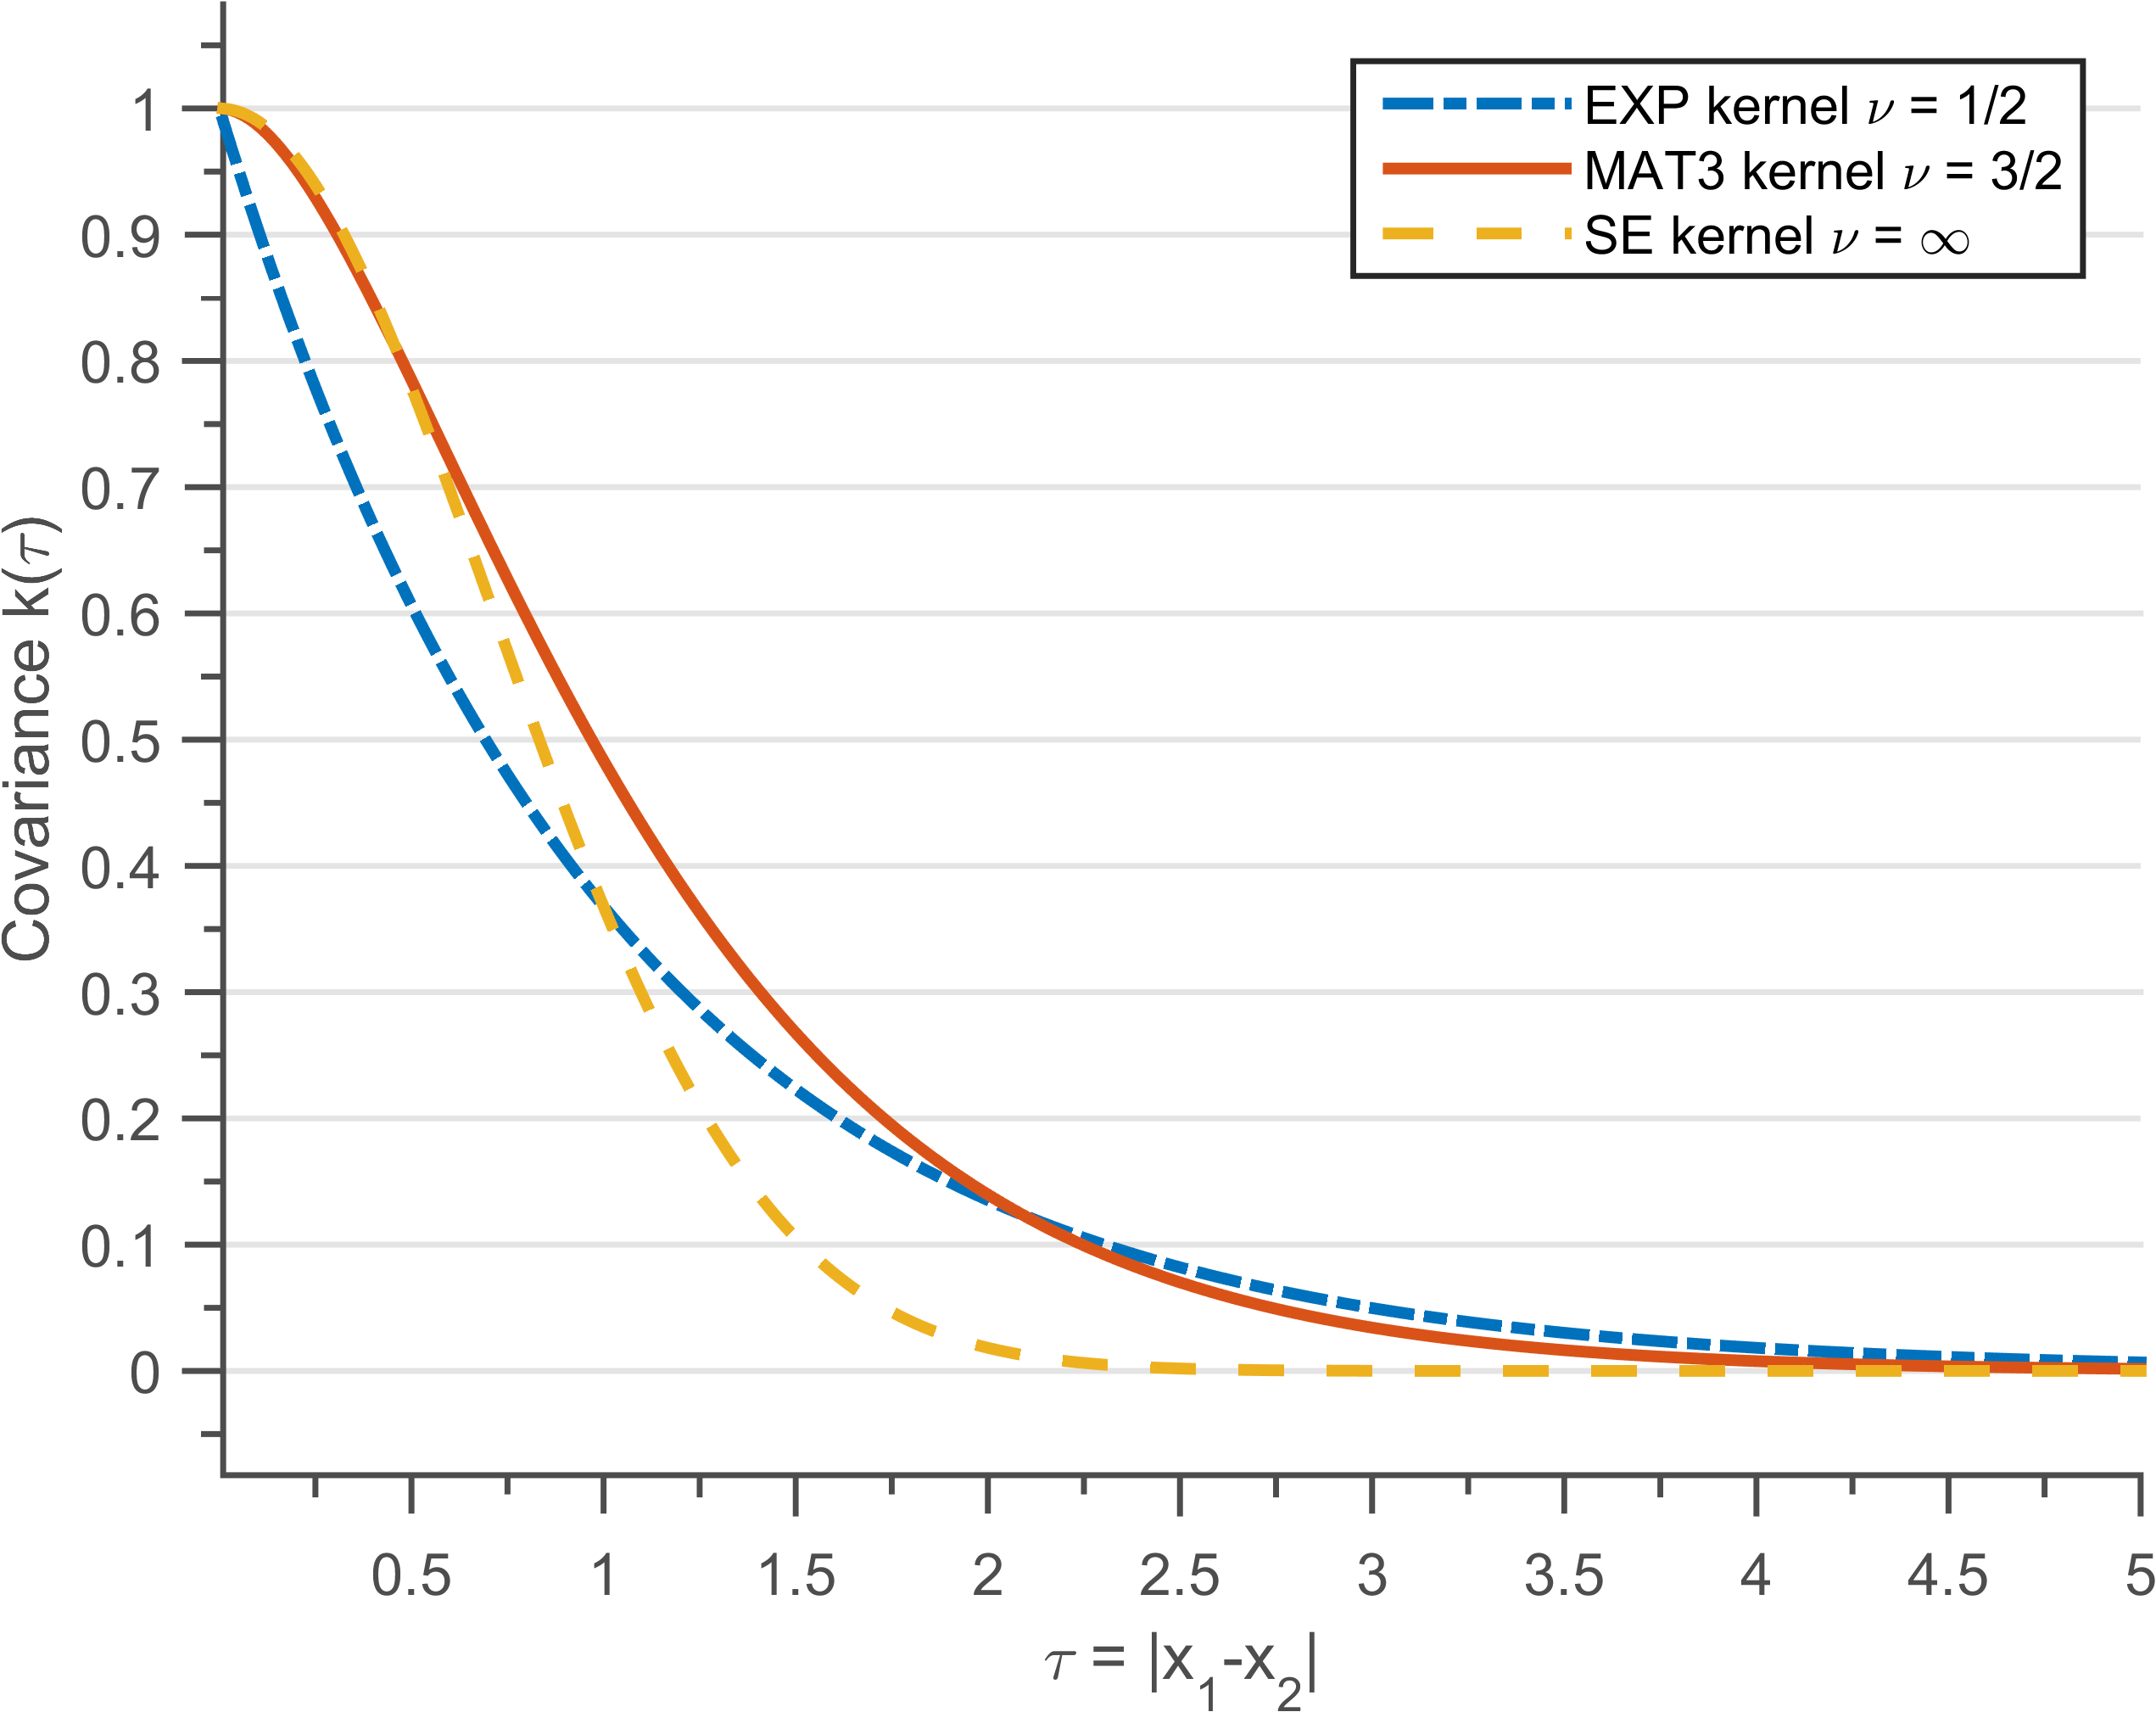
\includegraphics[width=0.45\textwidth]
        {imagesPart2/kernelFunctions}
        \label{subFigkernelFunctions}
  }\quad
\subfigure[{Power spectrum for Exponential, Mat\'ern (\(\nu=3/2\))and Standard exponential kernel. The hyper-parameters are amplitude (\(\theta_{amplitude} = 1\)) and length-scale (\(\theta_{lengthScale} = 1\)). Exponential and Mat\'ern have more power at higher frequencies when compared to SE kernel.}]
  {
        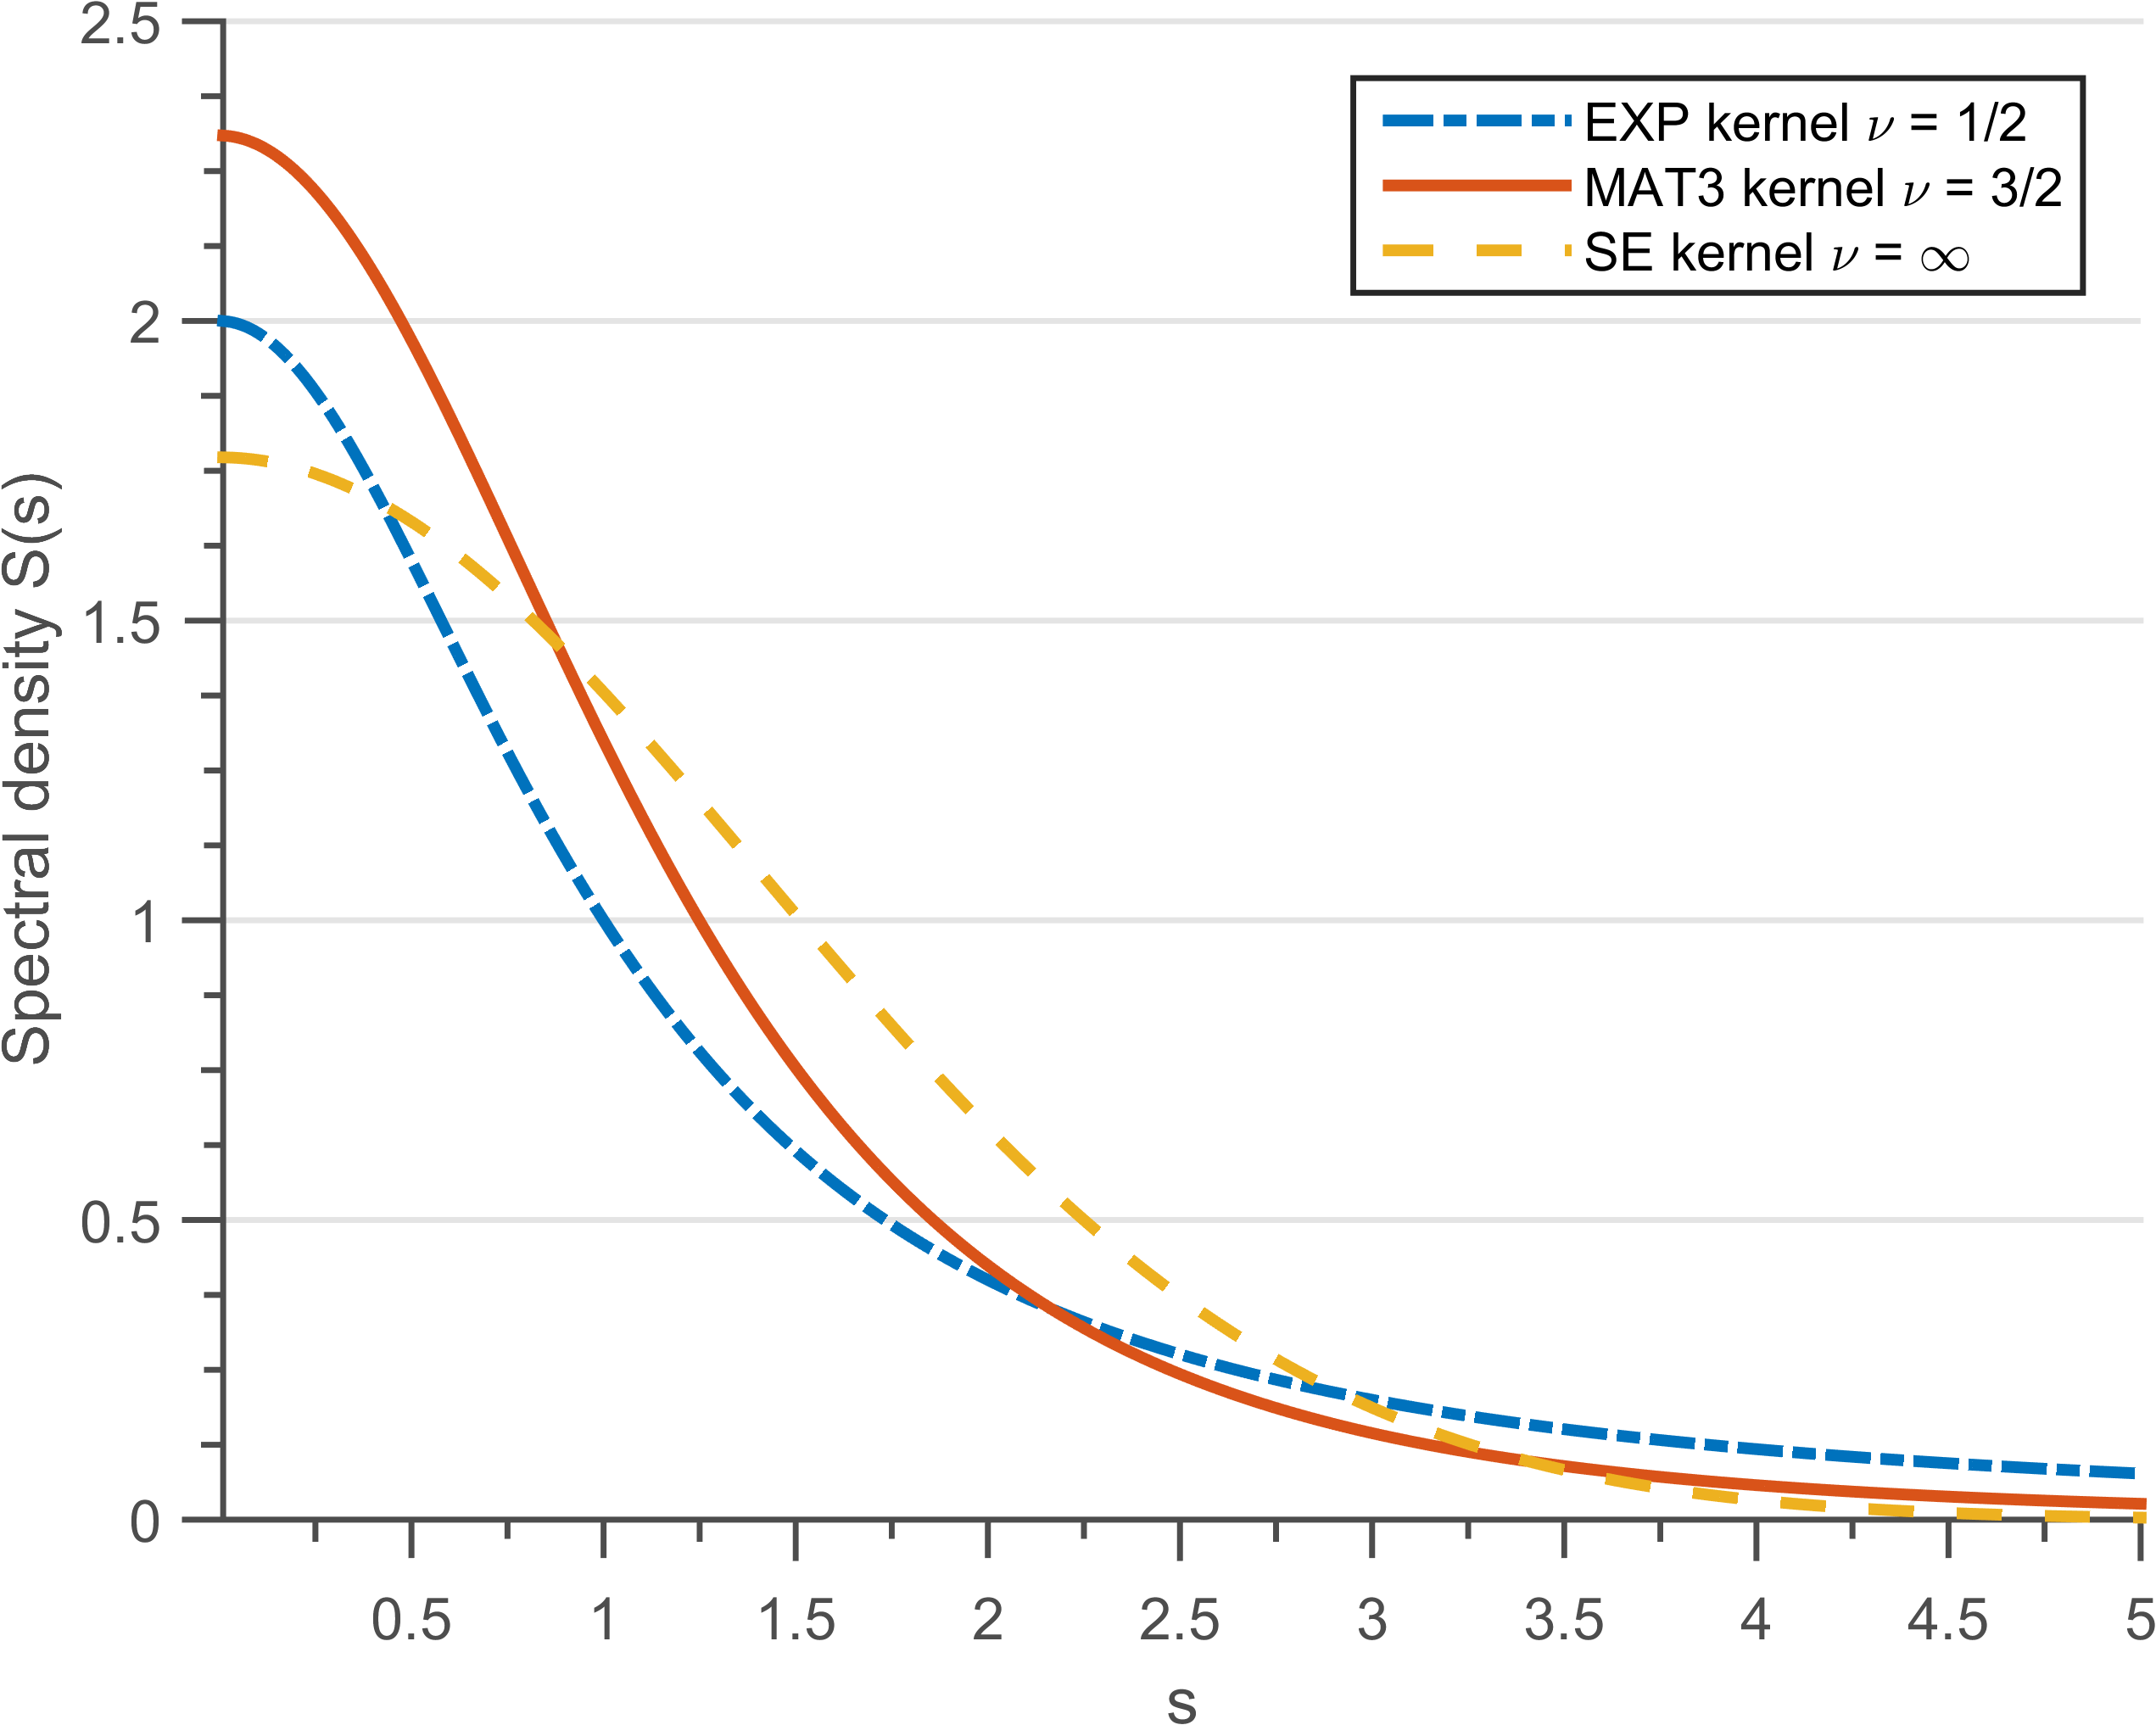
\includegraphics[width=0.45\textwidth]
        {imagesPart2/spectralFunctions}
        \label{subFigspectralFunctions}
  }\quad
\caption{Covariance functions and Power spectrums for three different kernels}
       \label{figKernelAndPowerSpectrums}
\end{figure}

The infinitely smooth assumption of the squared exponential function is unrealistic in several cases \cite{stein2012interpolation}, making the Mat\'ern kernels second most popular choice of kernels. Mat\'ern kernels have been found to have superior performance on datasets with high-dimensions \cite{le2013fastfood}. It is argued that the Mat\'ern kernel accounts for the concentration of measure effect in higher-dimensions. Imagine a high-dimensional orange (it is tough to imagine more than 3 dimensions), but if there was a high dimensional orange than most of its mass will be concentrated in its skin and not its pulp \cite{domingos2012few}. 

\subsection{Experiments}
Let us revisit the dataset \(\mathcal{D}_{2}\) used to calculate the posterior in section \ref{secPosterior} but this time using three different covariance functions. We will use Exponential kernel, Mat\'ern and Standard exponential kernel to compare their performance during GP regression. 

We follow the standard framework of GP regression, we first draw random functions from a the covariance functions to judge the hypothesis space. We next calculate the posterior distribution conditioned on dataset \(\mathcal{D}_{2}\). We finally, optimize the marginal likelihood and compare the final predictions for the three covariance functions. 

Figure \ref{figCh4Priors} shows 5 random functions drawn for a zero mean GP with the three covariance functions for same values of hyper-parameters \(\theta_{lengthscale} = 1, \theta_{amplitude} = 1\), their corresponding covariance functions and power spectrums are whown in figure \ref{figKernelAndPowerSpectrums}. The solid black line defines the mean function, shaded blue region defines 95\% confidence interval (2\(\sigma\)) distance away from the mean. The dashed lines are five functions drawn at random from a GP prior. We can observe that figure \ref{subFigpriorDrawsEXP} draws non-differentiable functions while \ref{subFigpriorDrawsMAT3} and \ref{subFigpriorDrawsSE} draw smoother functions. For the same value of the length-scale, Mat\'ern (\(\nu=3/2\)) kernel has higher variation.

\begin{figure}[!ht]
  \centering
    \subfigure[{Draws from a GP prior with mean zero, Exponential kernel (Mat\'ern with \(\nu = 1/2\)) and hyper-parameters \(\theta_{lengthscale} = 1, \theta_{amplitude} = 1\). Functions drawn from this kernel are non-differentiable.}]
  {
        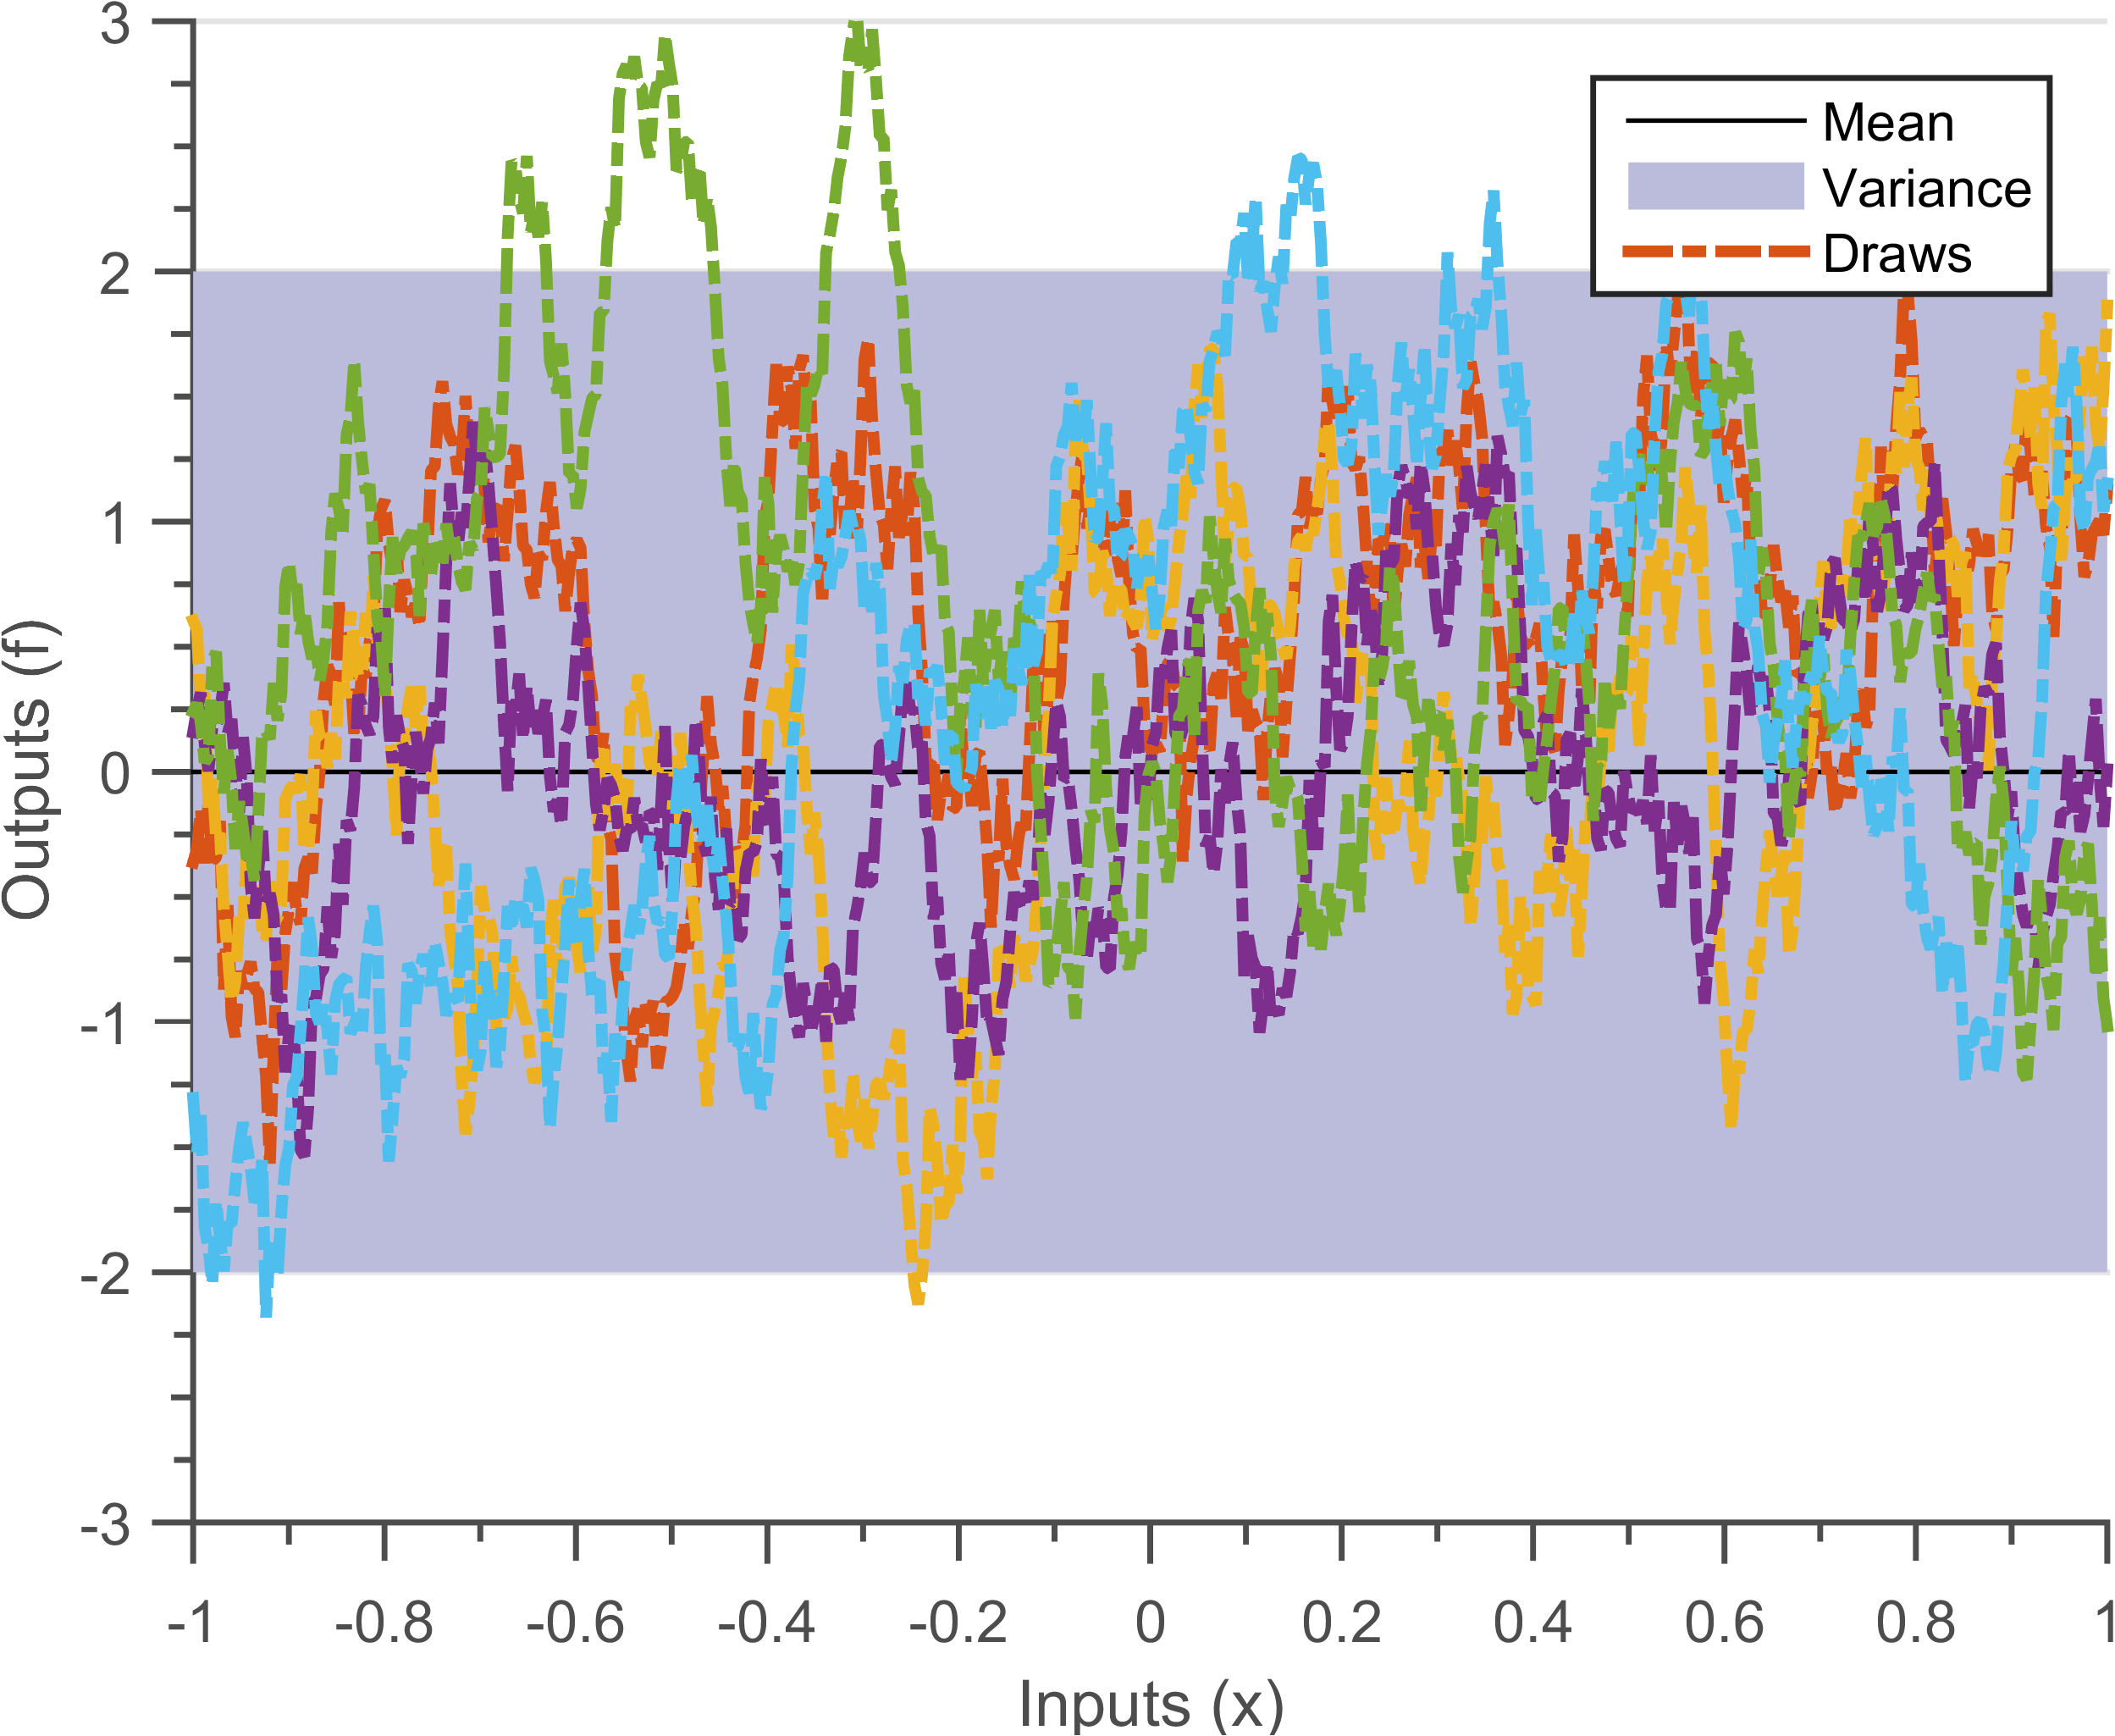
\includegraphics[width=0.29\textwidth]
        {imagesPart2/priorDrawsEXP}
        \label{subFigpriorDrawsEXP}
  }\quad
\subfigure[{Draws from a GP prior with mean zero, Mat\'ern kernel \(\nu = 3/2\) and hyper-parameters \(\theta_{lengthscale} = 1, \theta_{amplitude} = 1\). Functions drawn from this kernel are differentiable only once}]
  {
        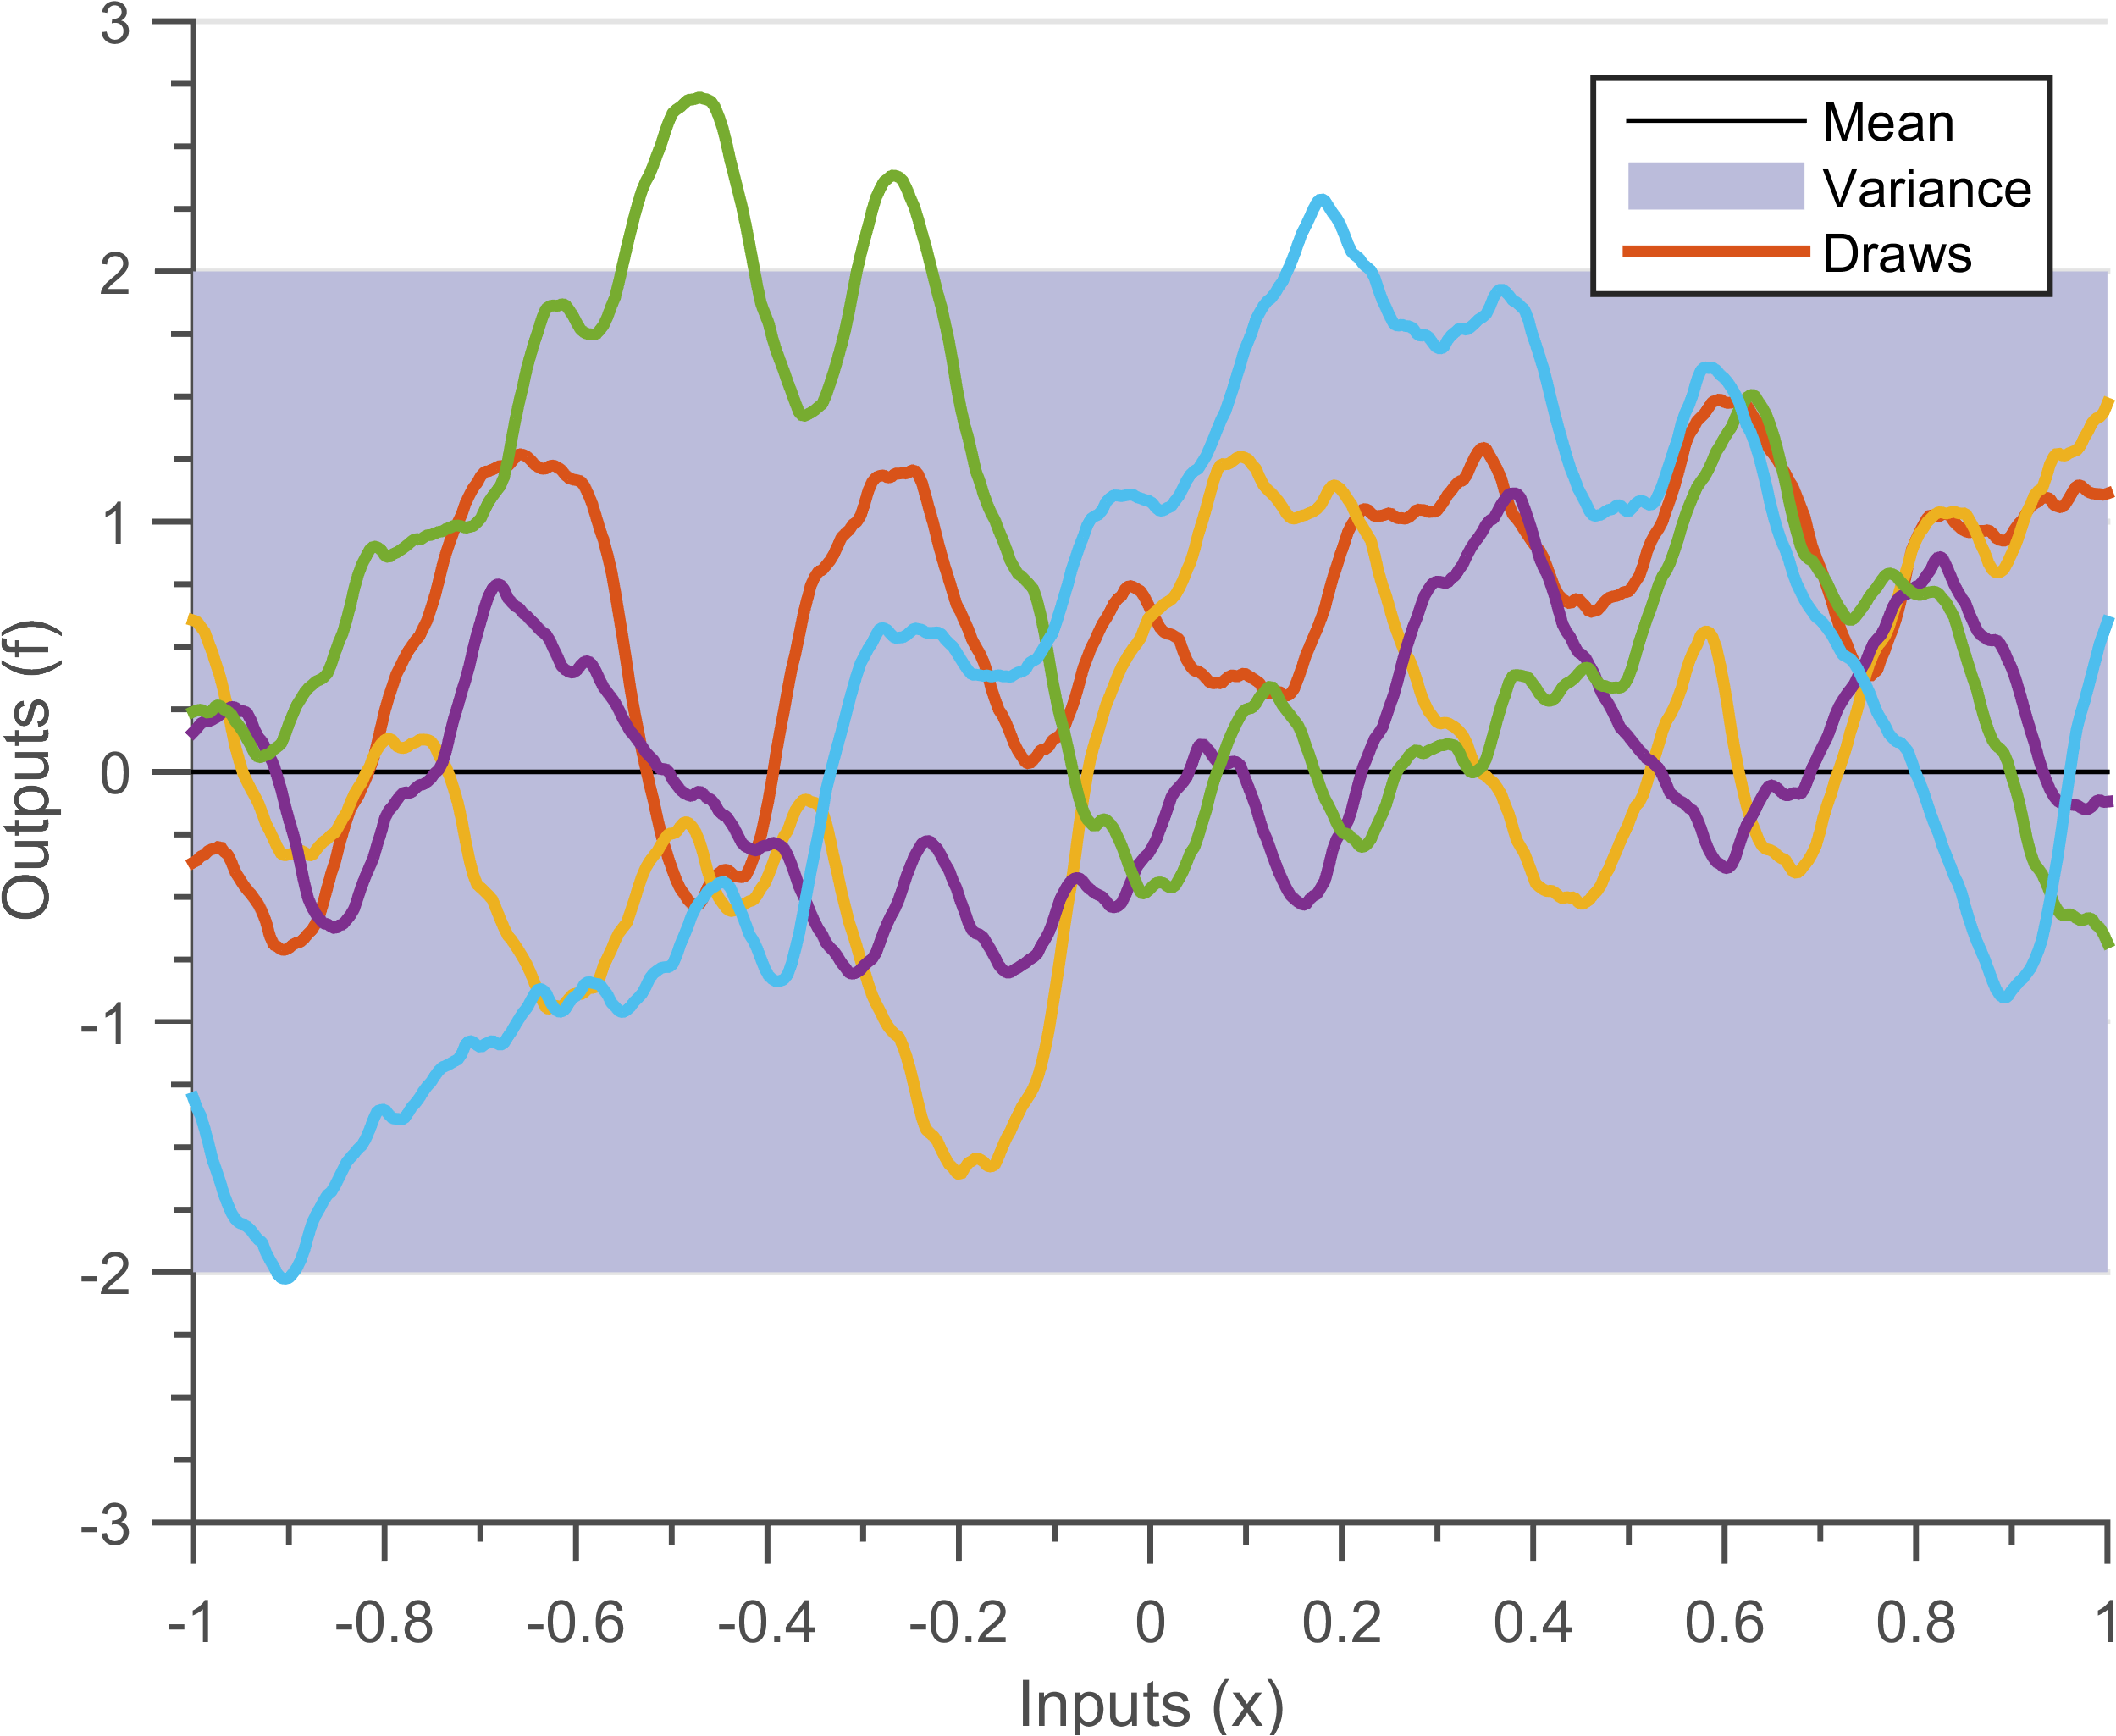
\includegraphics[width=0.29\textwidth]
        {imagesPart2/priorDrawsMAT3}
        \label{subFigpriorDrawsMAT3}
  }\quad
  \subfigure[{Draws from a GP prior with mean zero, Standard Exponential kernel (Mat\'ern with \(\nu = \infty\)) and hyper-parameters \(\theta_{lengthscale} = 1, \theta_{amplitude} = 1\). Functions drawn from this kernel are infinitely differentiable}]
  {
        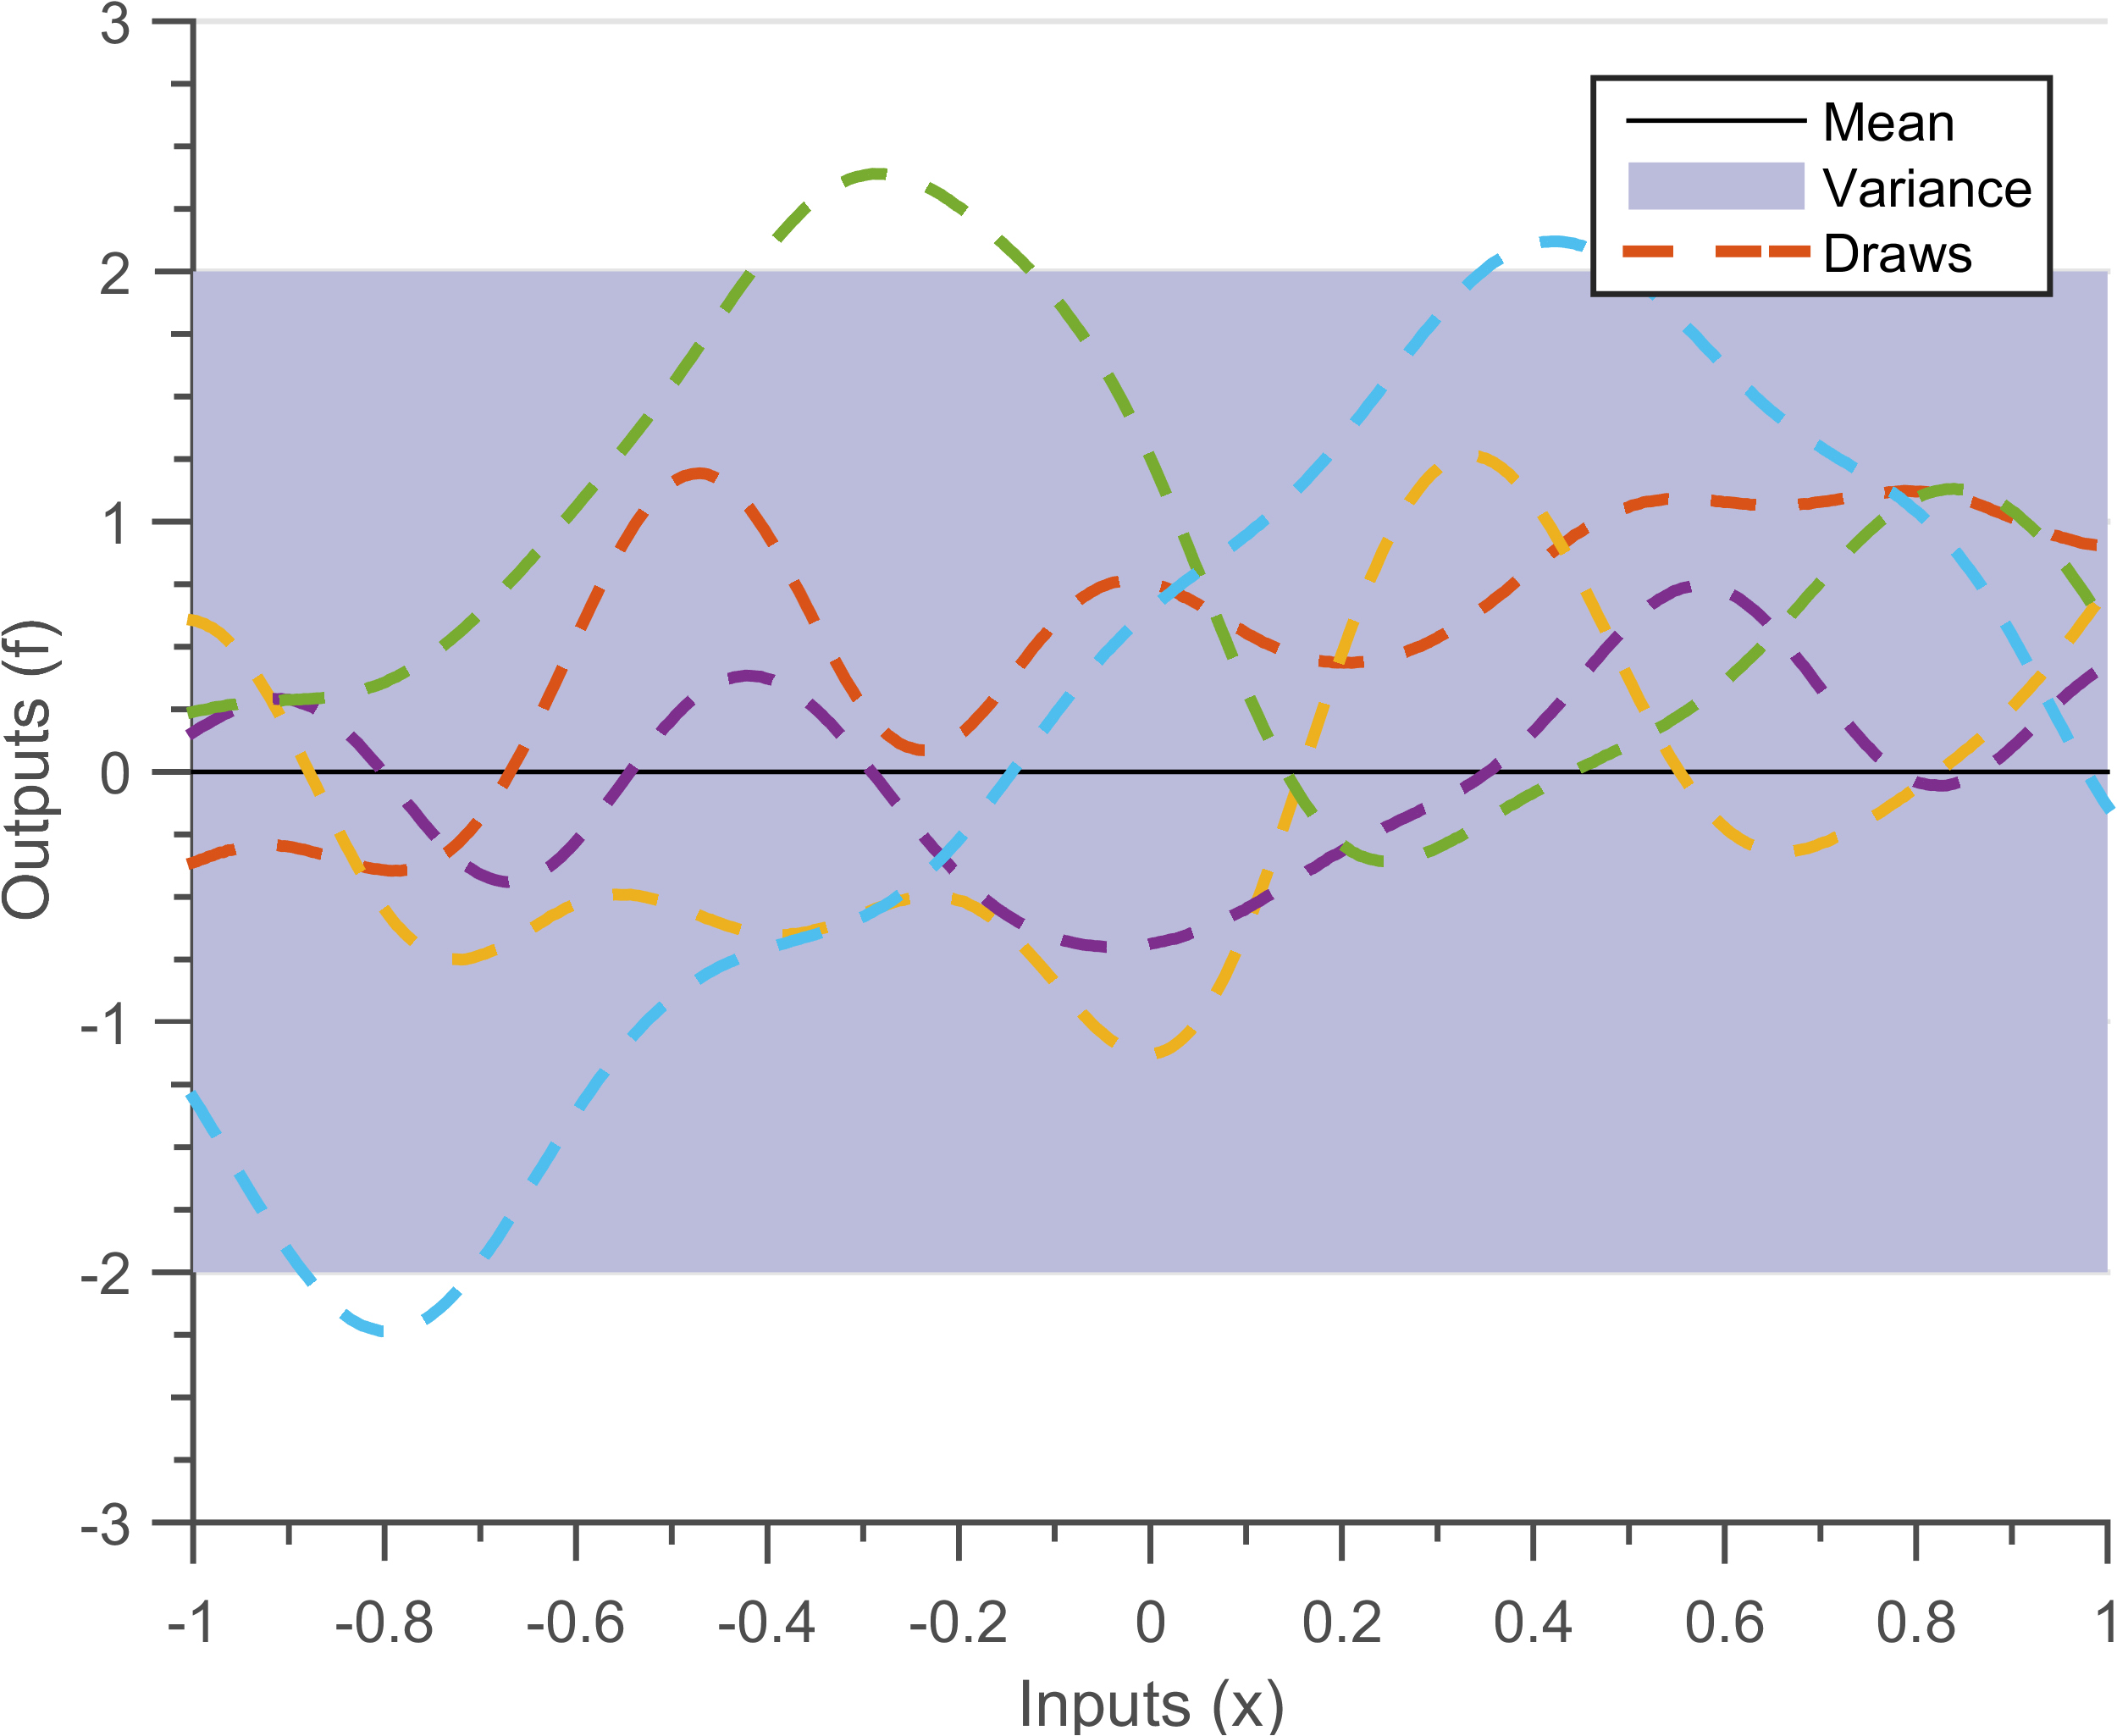
\includegraphics[width=0.29\textwidth]
        {imagesPart2/priorDrawsSE}
        \label{subFigpriorDrawsSE}
  }\quad
\caption{Prior distribution and five random draws from 3 different covariance functions. The solid black line defines the mean function, shaded blue region defines 95\% confidence interval (2\(\sigma\)) distance away from the mean. The dashed lines are five functions drawn at random from a GP prior.}
       \label{figCh4Priors}
\end{figure}

Figure \ref{figpreOptimizedPosteriorCh5} shows the posterior GP conditioned on the dataset \(\mathcal{D}_{2}\) for three different covariance functions with same hyper-parameters. The hyper-parameters are not optimized with respect to the marginal likelihood. For a similar value of hyper-parameters and dataset, Exponential kernel has highest variance followed by Mat\'ern and SE kernel\footnote{Remember the Bias vs Variance trade-off: SE kernel has the most restrictive hypothesis space followed by Mat\'ern \(\nu=3/2\) and Exponential kernel, since infinite differentiability is a stricter assumption}. 

\begin{figure}[!ht]
  \centering
    \subfigure[{Draws from a GP posterior with mean zero and Exopnential kernel (figure \ref{subFigpriorDrawsEXP}) conditioned on the data \(\mathcal{D}_{2}\). The posterior mean passes through the data points, random functions drawn from exponential kernel are non-differentiable}]
  {
        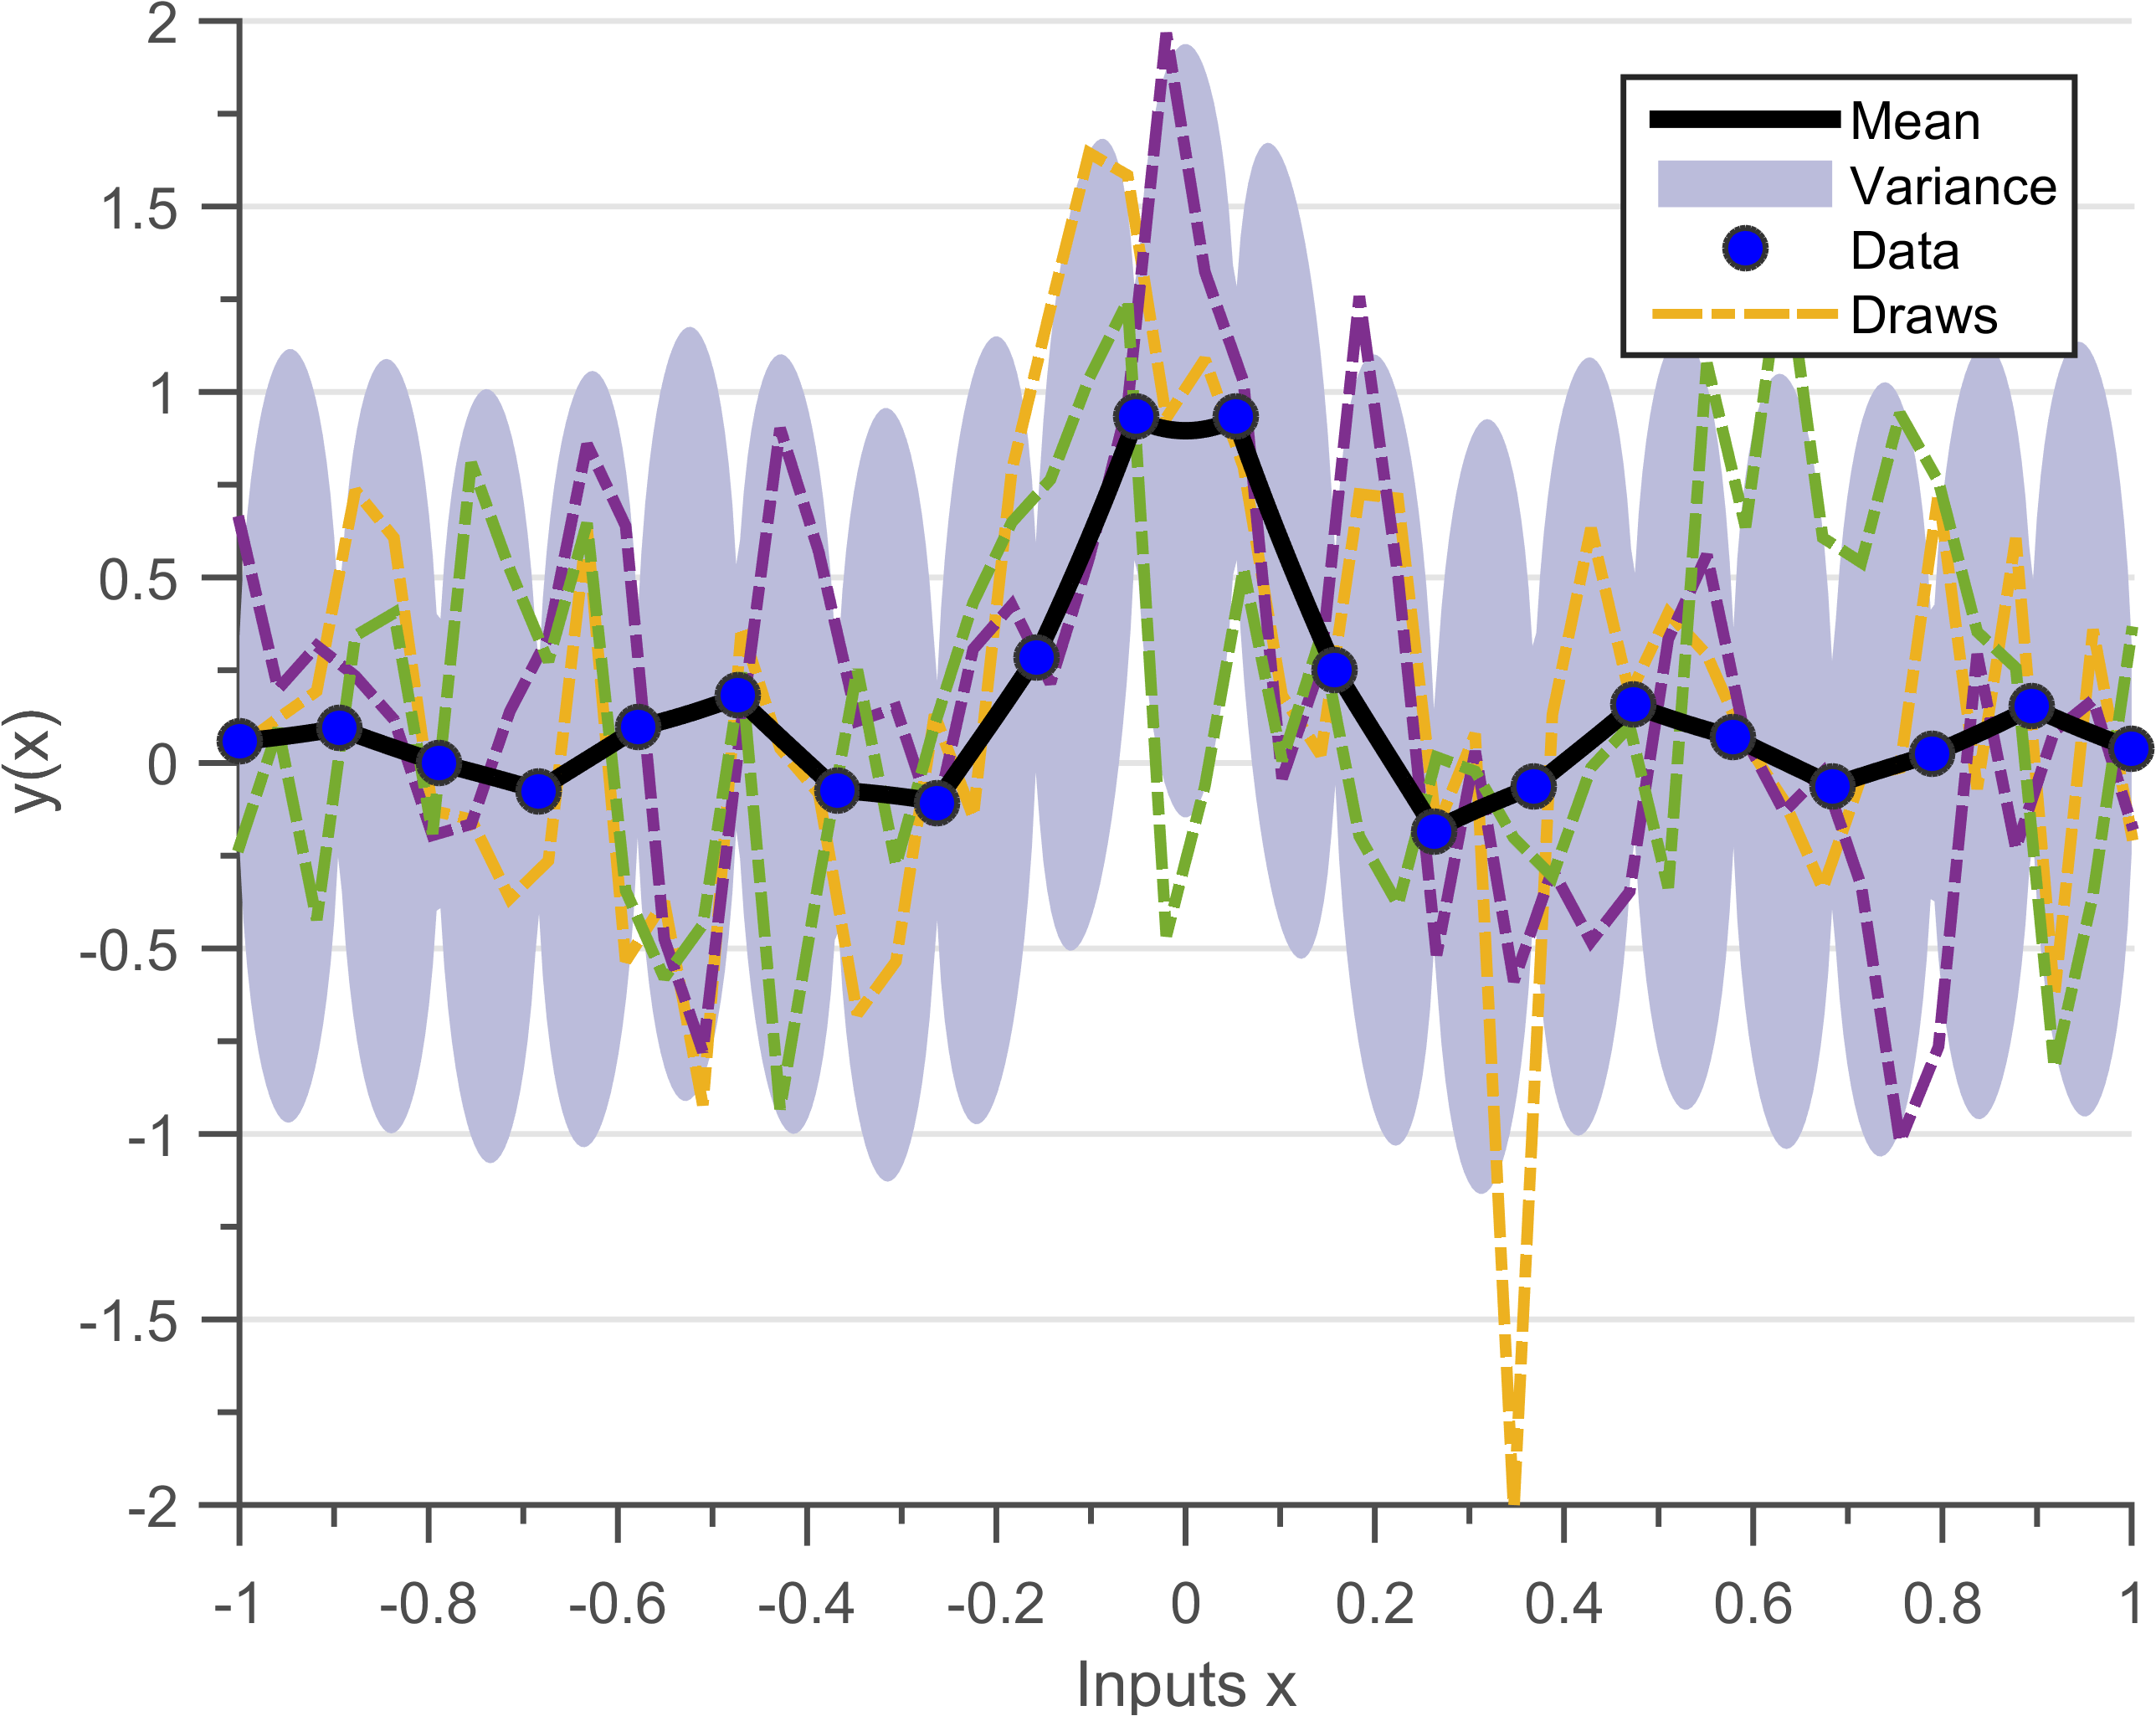
\includegraphics[width=0.29\textwidth]
        {imagesPart2/drawsPosteriorEXP}
        \label{subFigdrawsPosteriorEXP}
  }\quad
\subfigure[{Draws from a GP posterior with mean zero and Mat\'ern kernel \(\nu = 3/2\) (figure \ref{subFigpriorDrawsMAT3}) conditioned on the data \(\mathcal{D}_{2}\). The posterior mean passes through the data points, random functions drawn from this kernel are differentiable only once}]
  {
        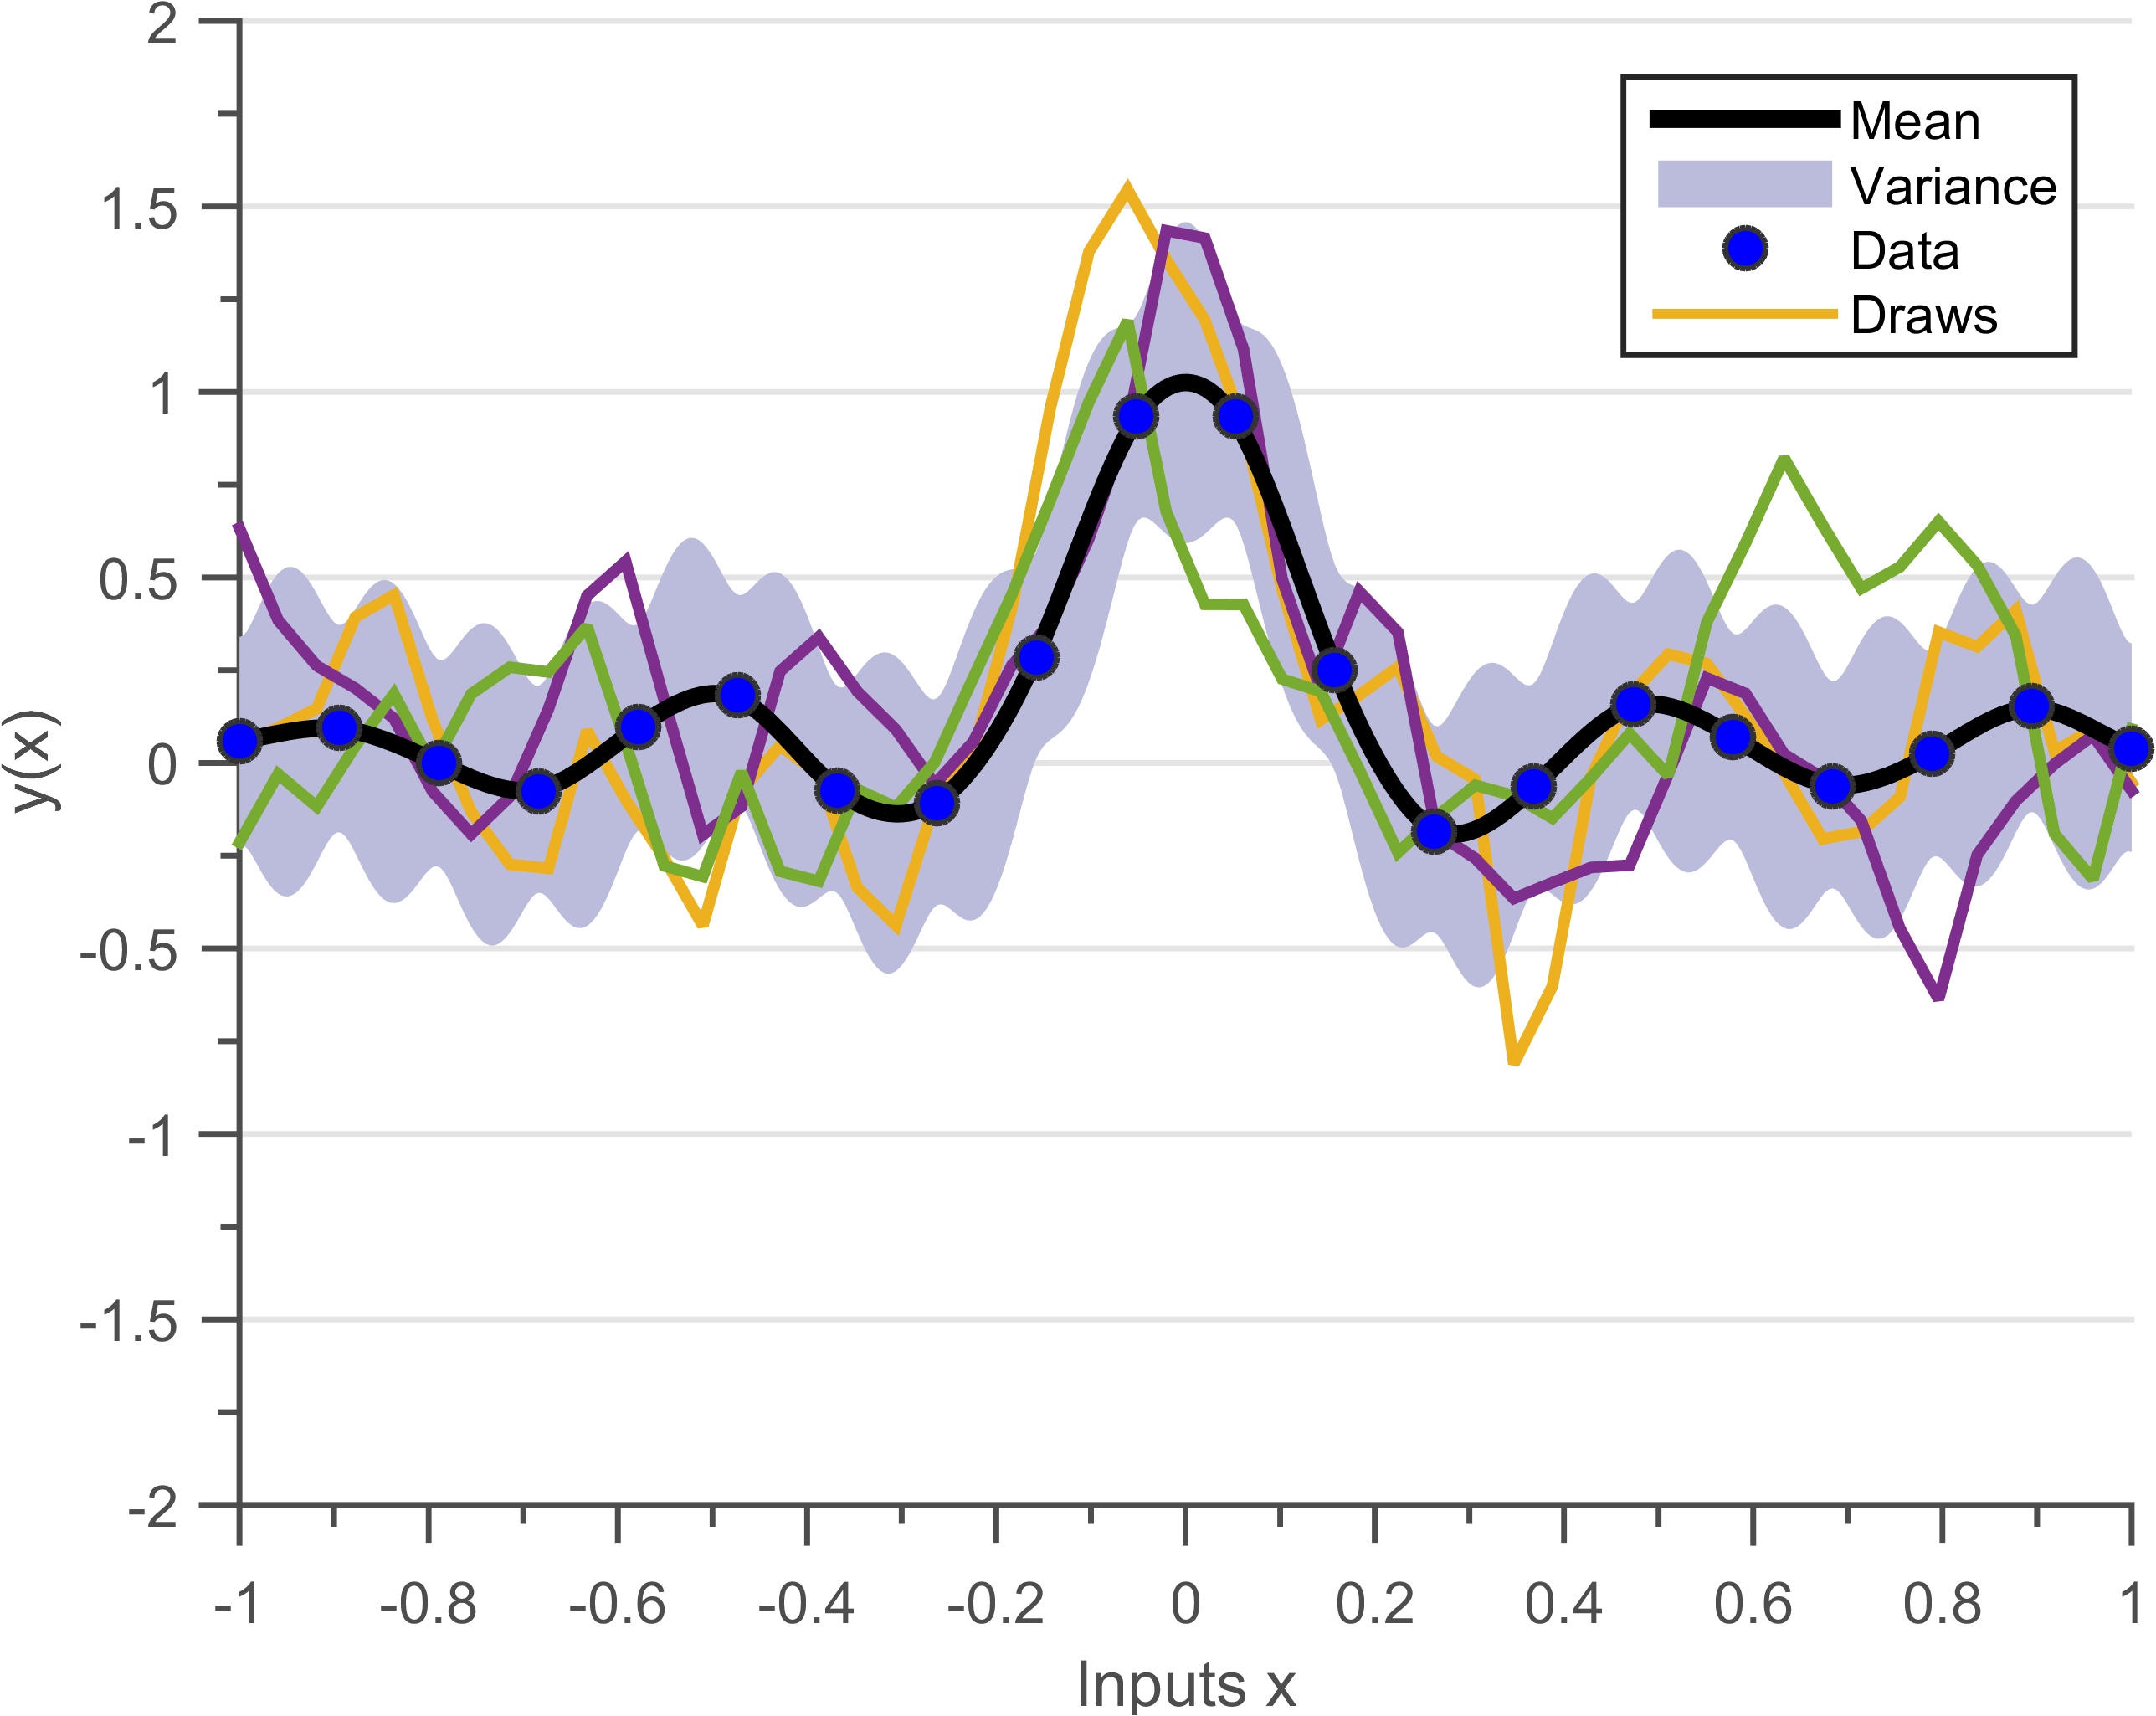
\includegraphics[width=0.29\textwidth]
        {imagesPart2/drawsPosteriorMAT3}
        \label{subFigdrawsPosteriorMAT3}
  }\quad
  \subfigure[{Draws from a GP posterior with mean zero and Standard exponential kernel \(\nu = \infty\) (figure \ref{subFigpriorDrawsMAT3}) conditioned on the data \(\mathcal{D}_{2}\). The posterior mean passes through the data points, random functions drawn from exponential kernel are infinitely differentiable}]
  {
        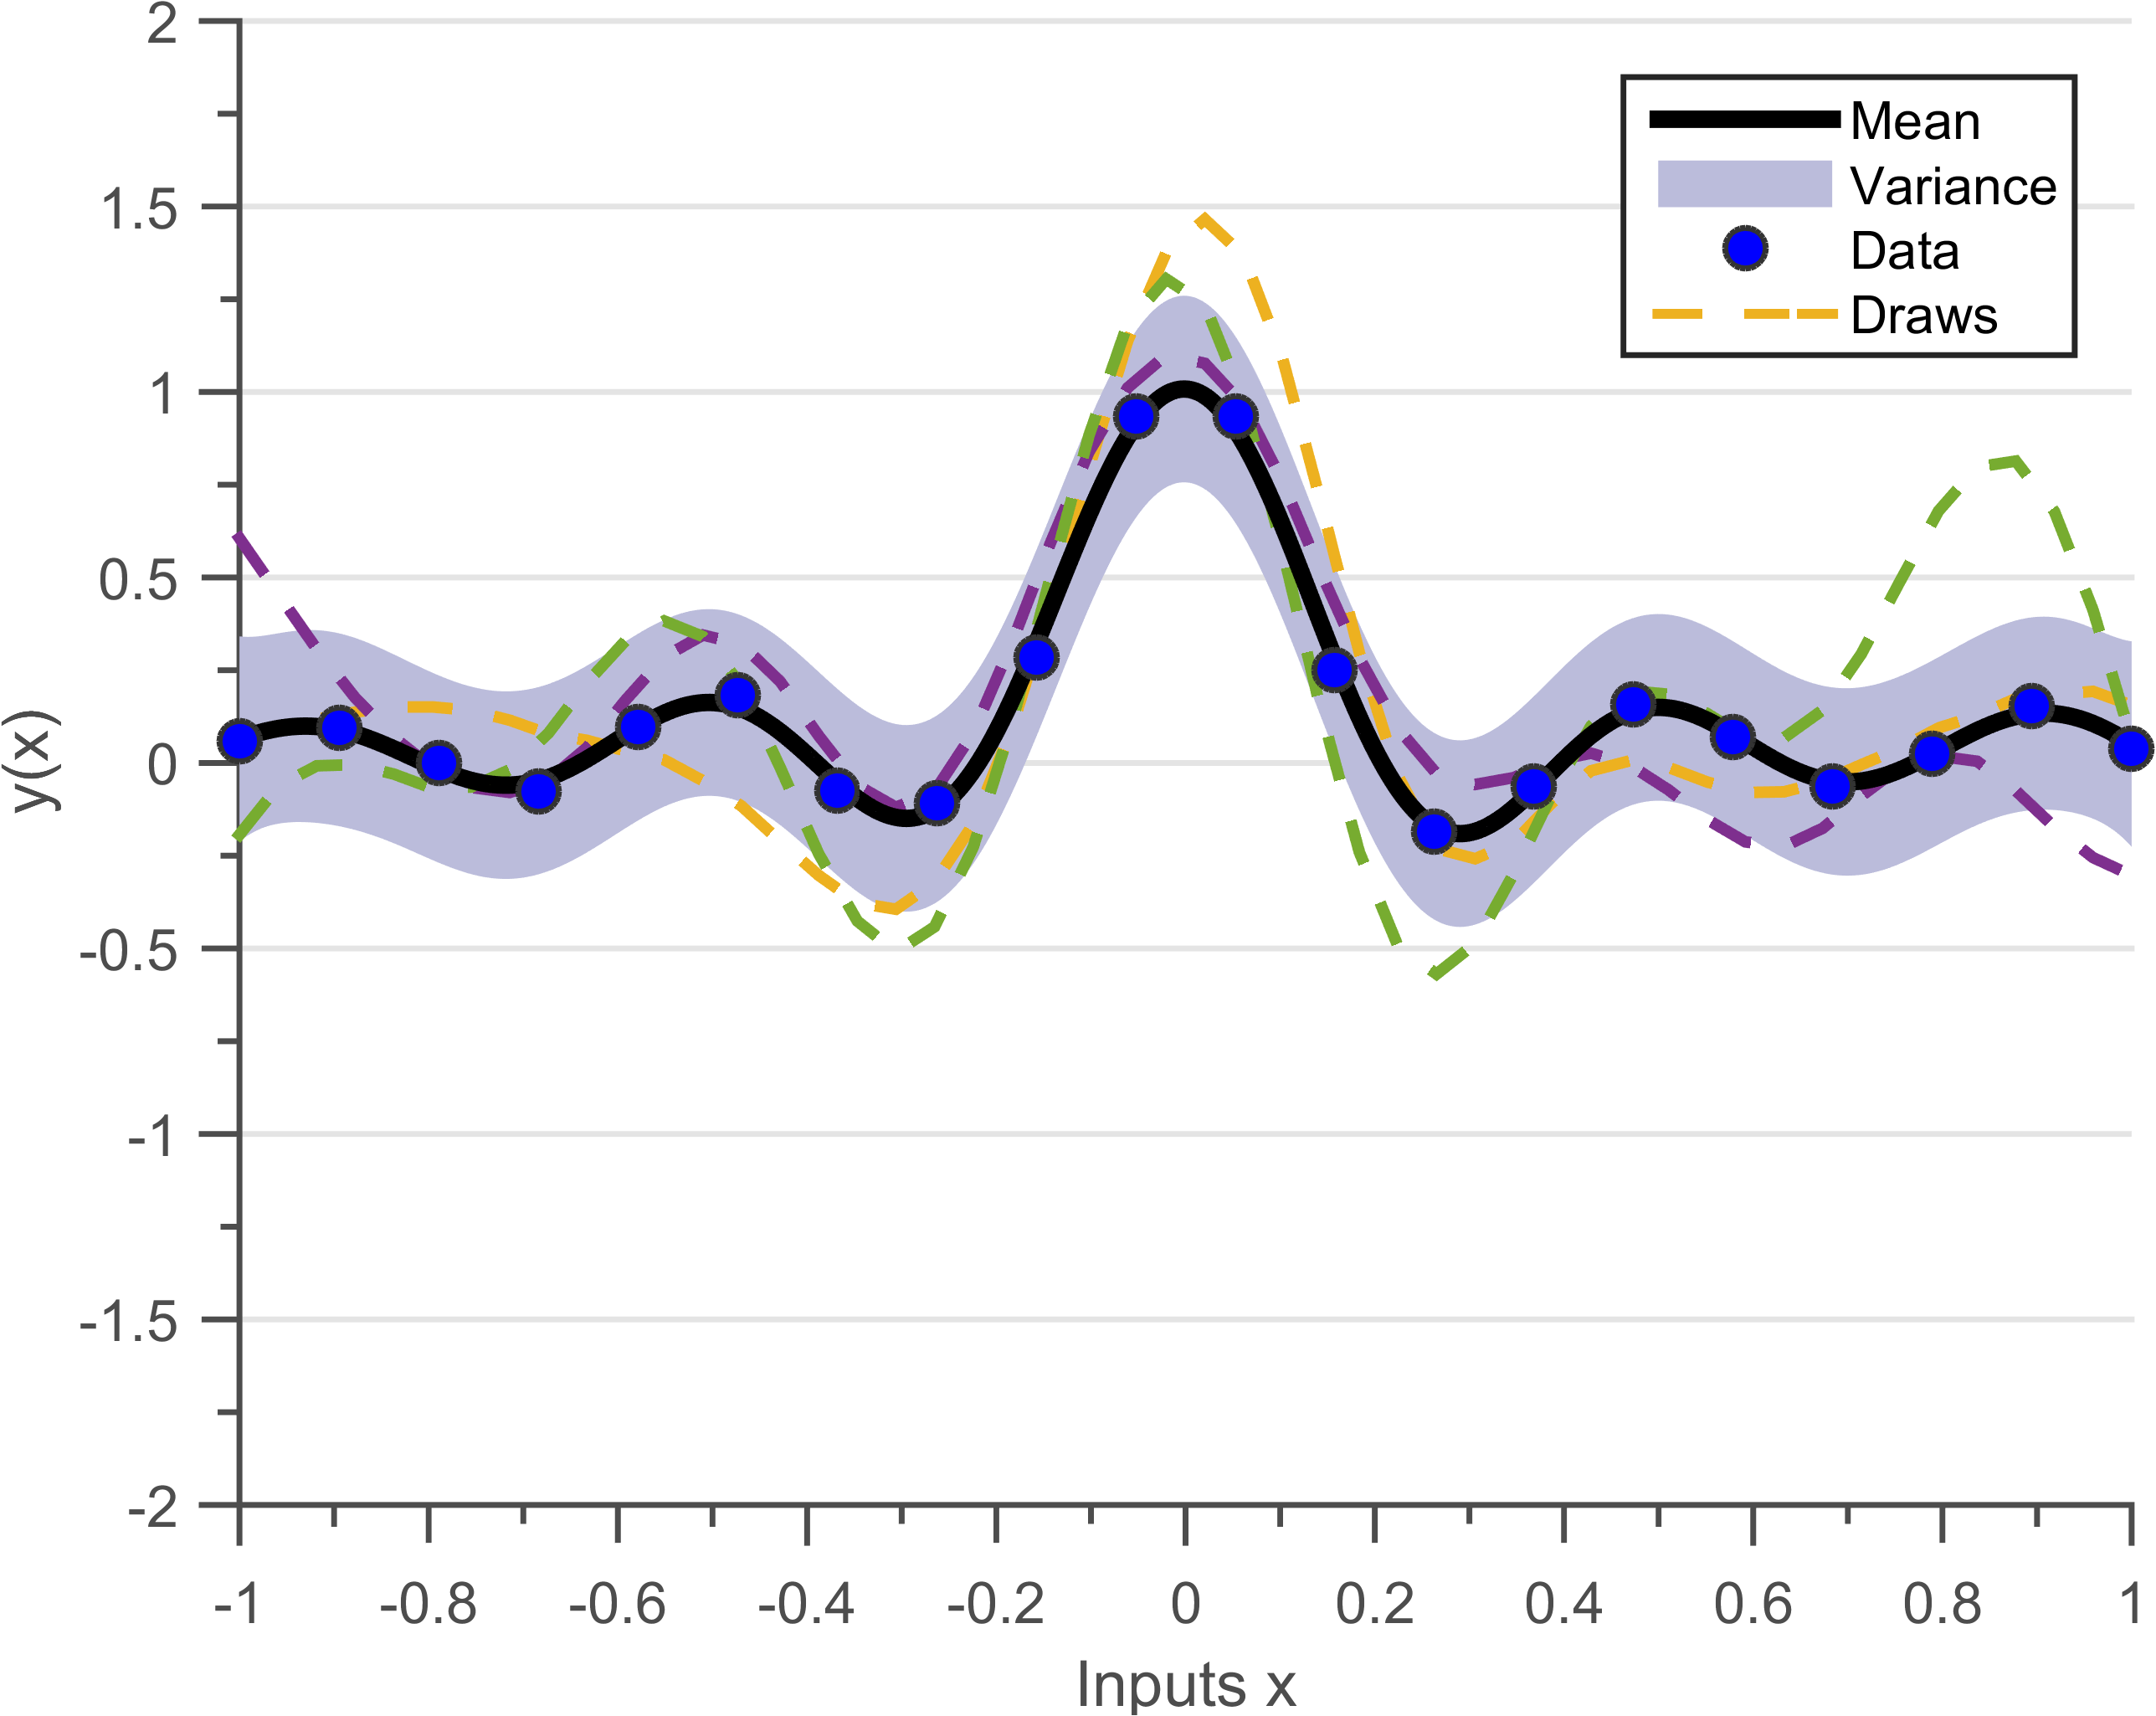
\includegraphics[width=0.29\textwidth]
        {imagesPart2/drawsPosteriorSE}
        \label{subFigdrawsPosteriorSE}
  }\quad
\caption{Posterior distribution and three random draws from 3 different covariance functions. The solid black line defines the mean function, shaded blue region defines 95\% confidence interval (2\(\sigma\)) distance away from the mean. The dashed lines are five functions drawn at random from a GP prior. }
       \label{figpreOptimizedPosteriorCh5}
\end{figure}


Figure \ref{figOptimizedPosteriorCh4} shows the posterior GP conditioned on the dataset \(\mathcal{D}_{2}\) for three different covariance functions with optimized hyper-parameters. This experiment only shows the different posteriors obtained for same observational data and different functional forms of the covariance function. All three predictions can be the correct interpolations depending on the type of experiment, this is where engineering judgment is required. For example, if the dataset \(\mathcal{D}_{2}\) was sampled from a Brownian motion then figure \ref{subFigdrawsOptimizedPosteriorEXP} would be the best fit. 

\begin{figure}[!ht]
  \centering
    \subfigure[{Draws from a GP posterior, conditioned on the dataset \(\mathcal{D}_{1}\) with mean zero and Exponential kernel with hyper-parameters (\(\theta_{lengthscale} = 0.215\), \(\theta_{amplitude} = 0.312\) and \(\sigma_{n} = 2.8e^-5\)) that maximize the marginal likelihood \(max(ML) = -1\).}]
  {
        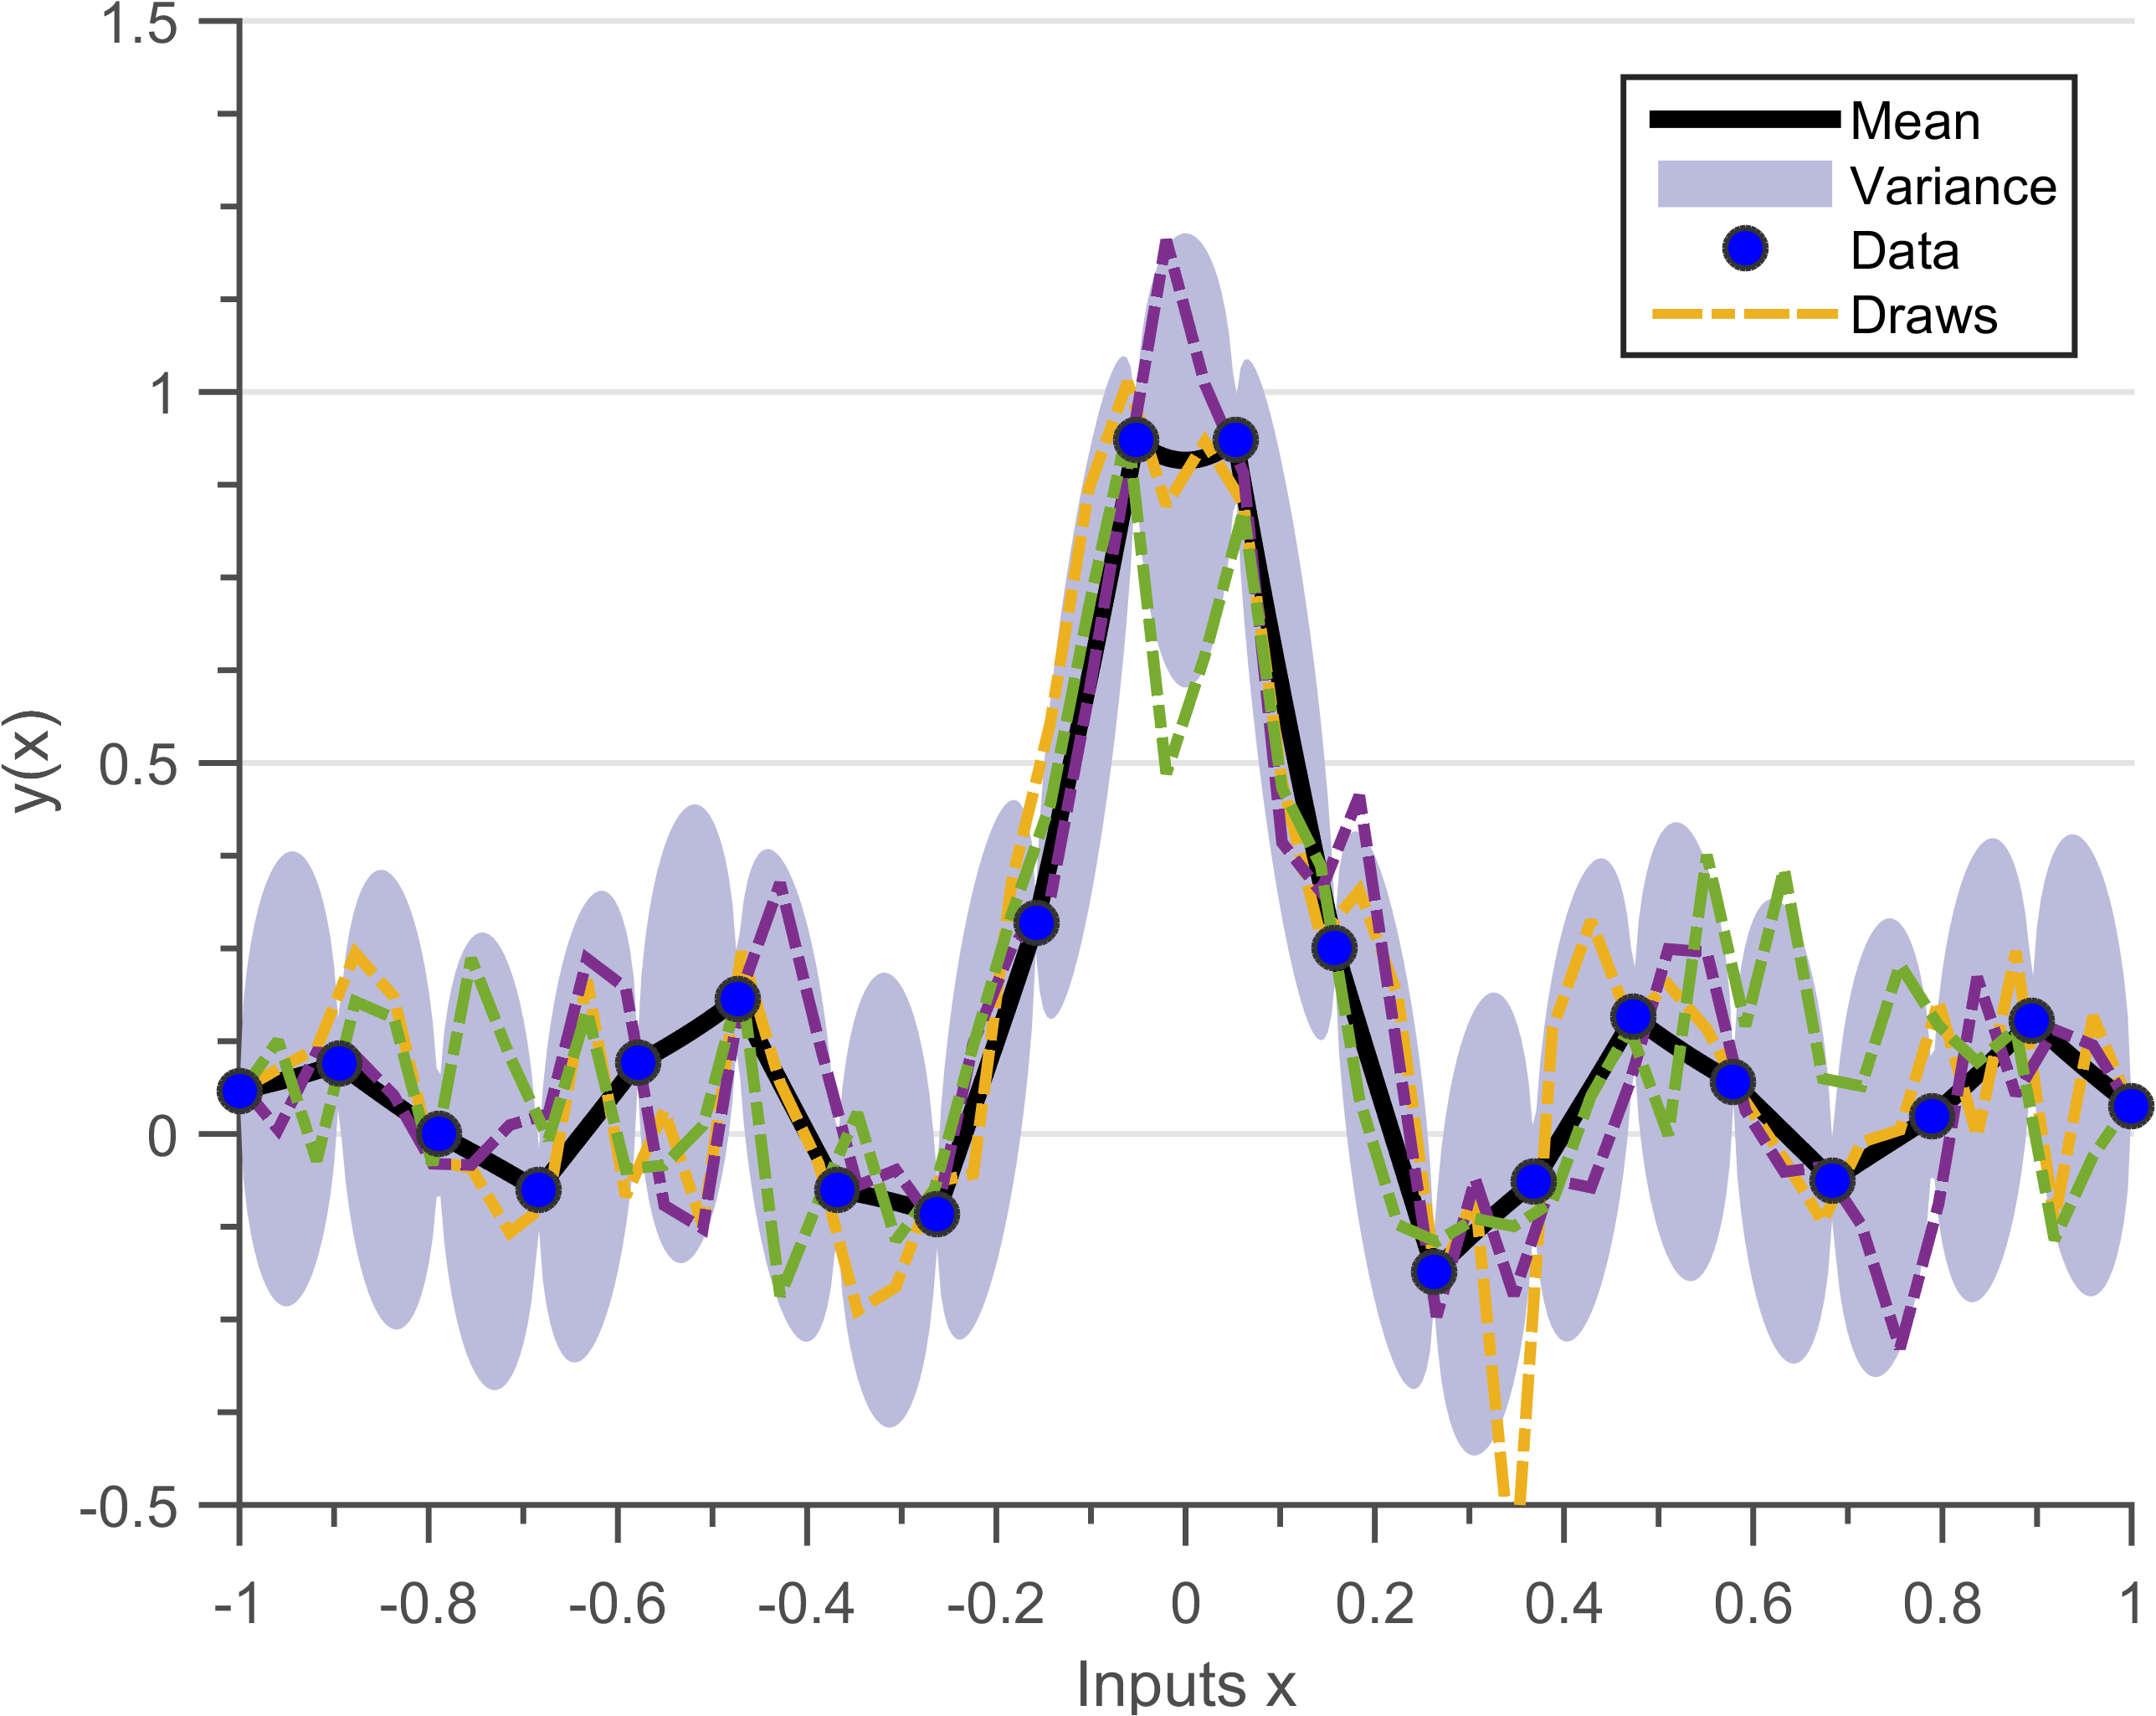
\includegraphics[width=0.29\textwidth]
        {imagesPart2/drawsOptimizedPosteriorEXP}
        \label{subFigdrawsOptimizedPosteriorEXP}
  }\quad
\subfigure[{Draws from a GP posterior, conditioned on the dataset \(\mathcal{D}_{1}\) with mean zero and Mat\'ern (\(\nu=3/2\)) kernel with hyper-parameters (\(\theta_{lengthscale} = 0.2\), \(\theta_{amplitude} = 0.347\) and \(\sigma_{n} = 1.7e^-5\)) that maximize the marginal likelihood \(max(ML) = 2\)}]
  {
        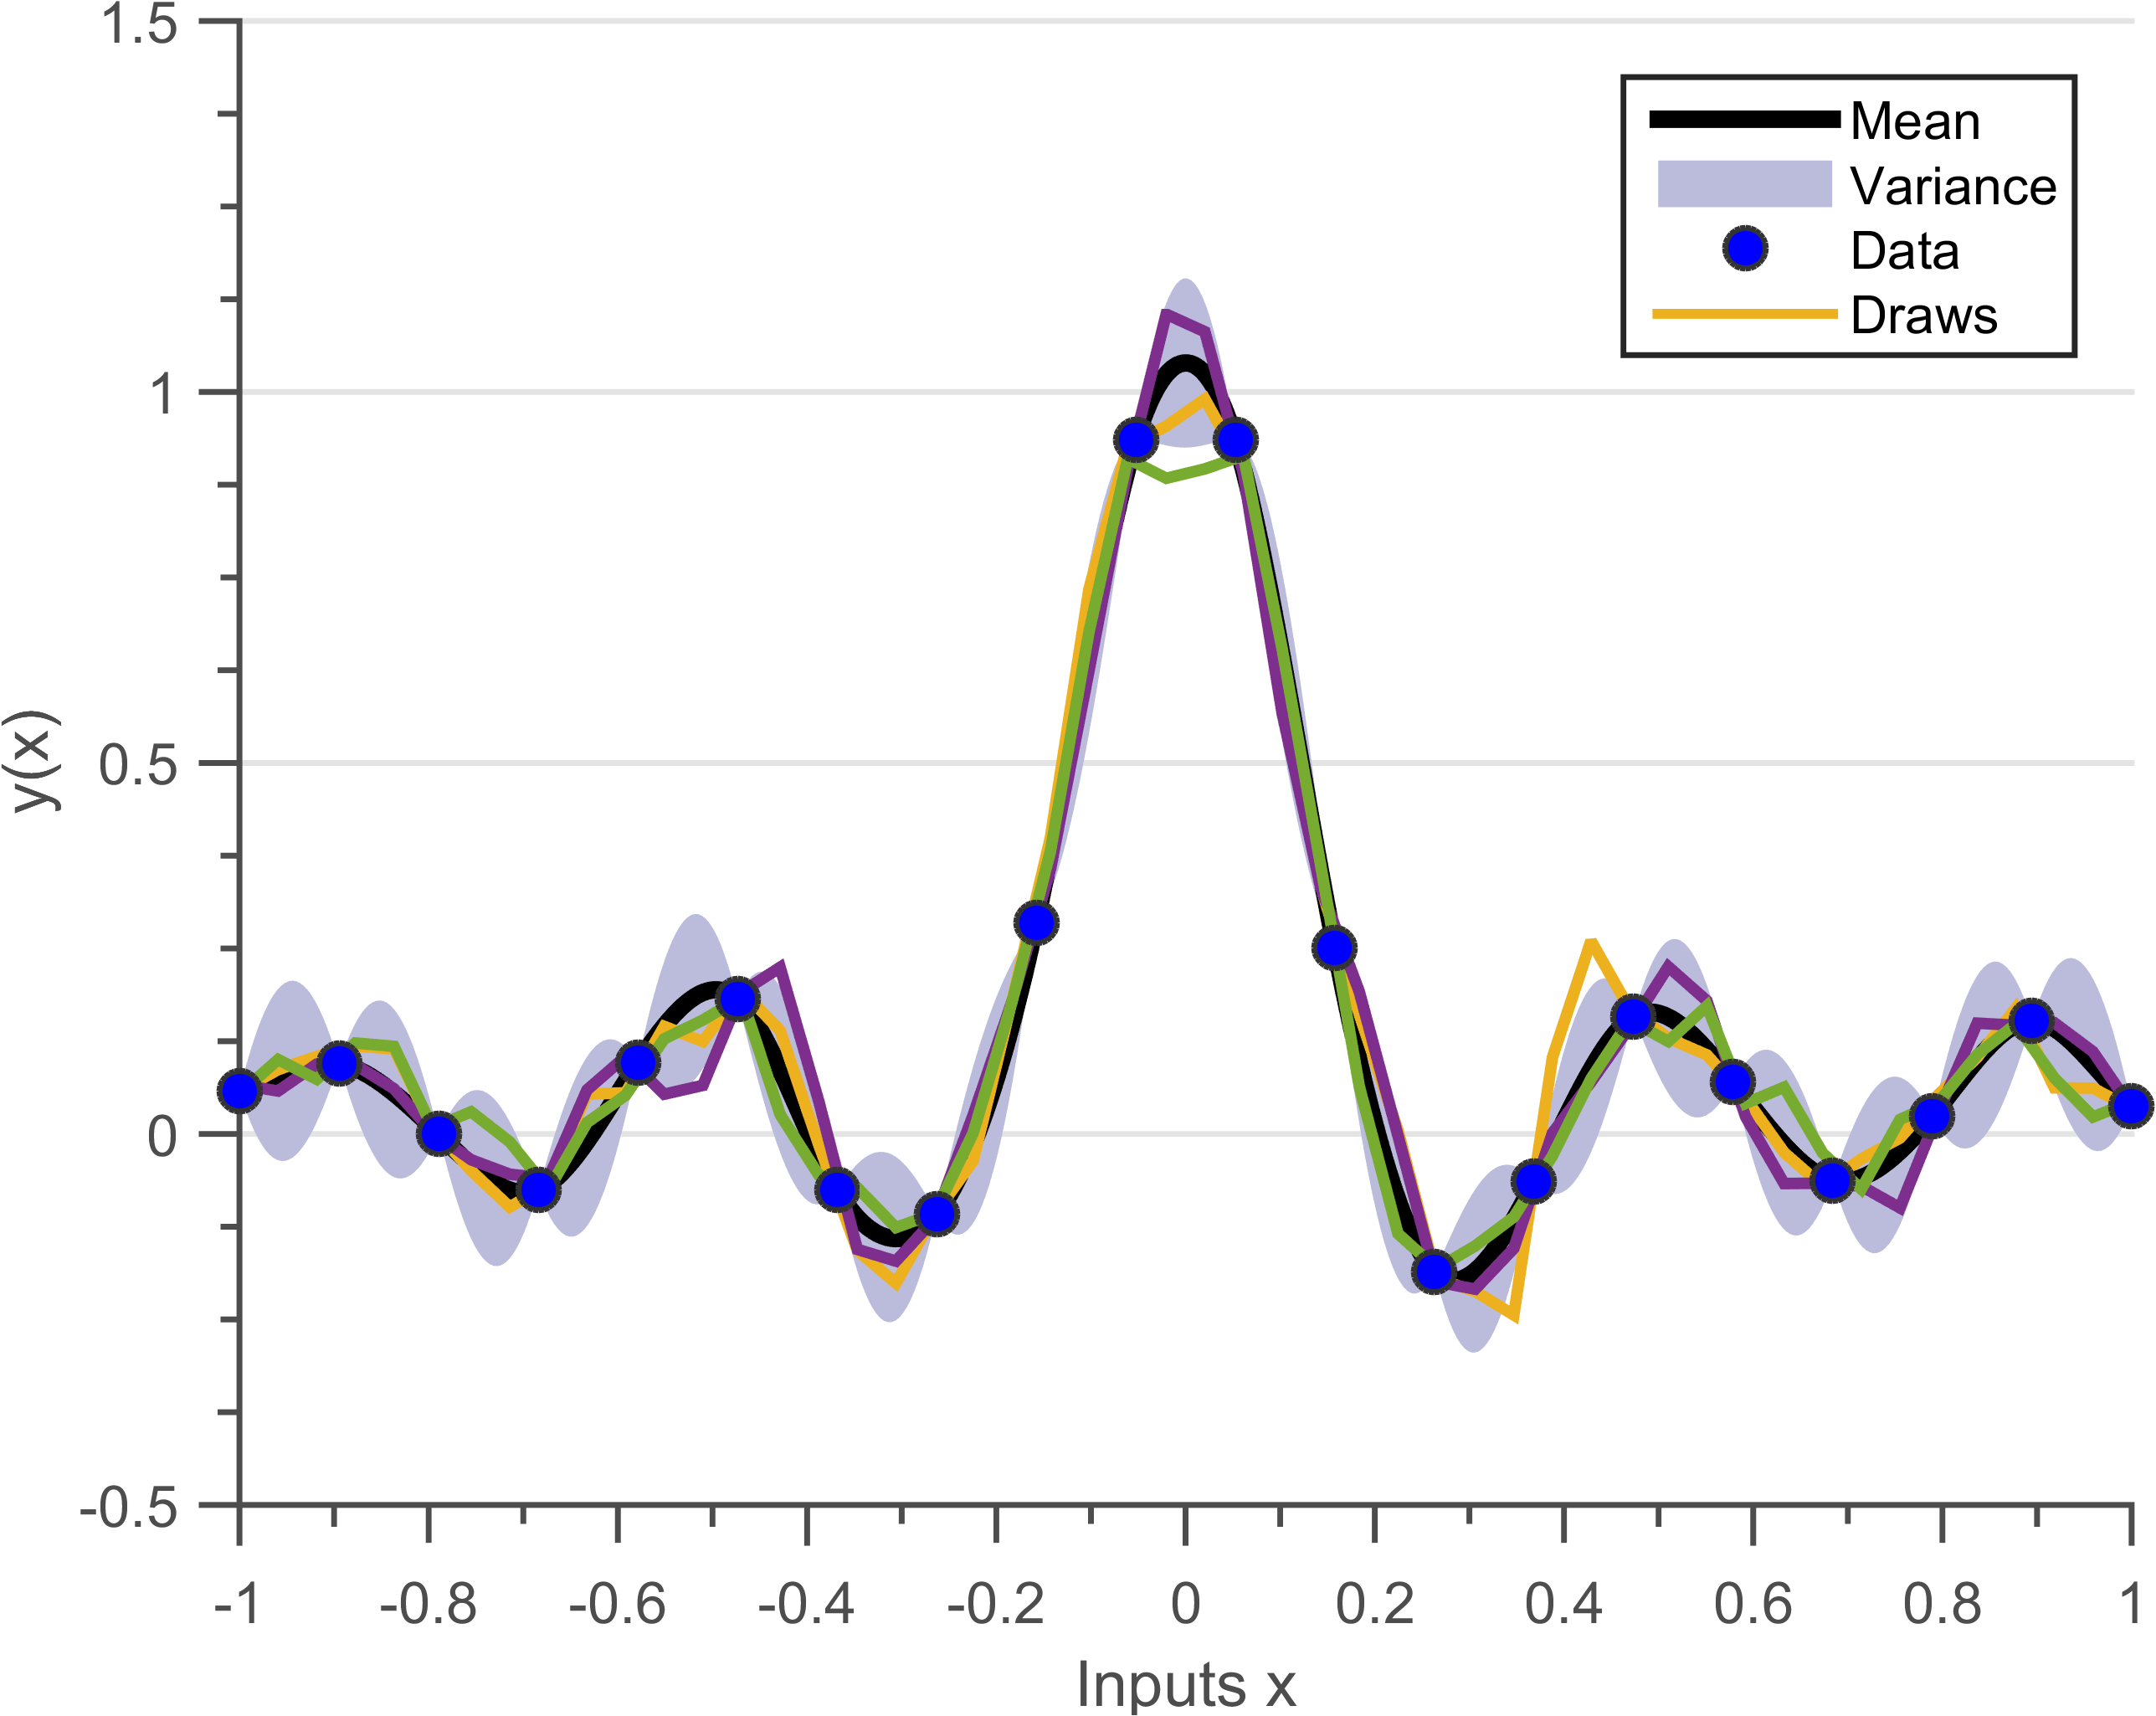
\includegraphics[width=0.29\textwidth]
        {imagesPart2/drawsOptimizedPosteriorMAT3}
        \label{subFigdrawsOptimizedPosteriorMAT3}
  }\quad
  \subfigure[{Draws from a GP posterior, conditioned on the dataset \(\mathcal{D}_{1}\) with mean zero and se kernel with hyper-parameters (\(\theta_{lengthscale} = 0.151\), \(\theta_{amplitude} = 0.358\) and \(\sigma_{n} = 0.01\)) that maximize the marginal likelihood \(max(ML) = 8\)}]
  {
        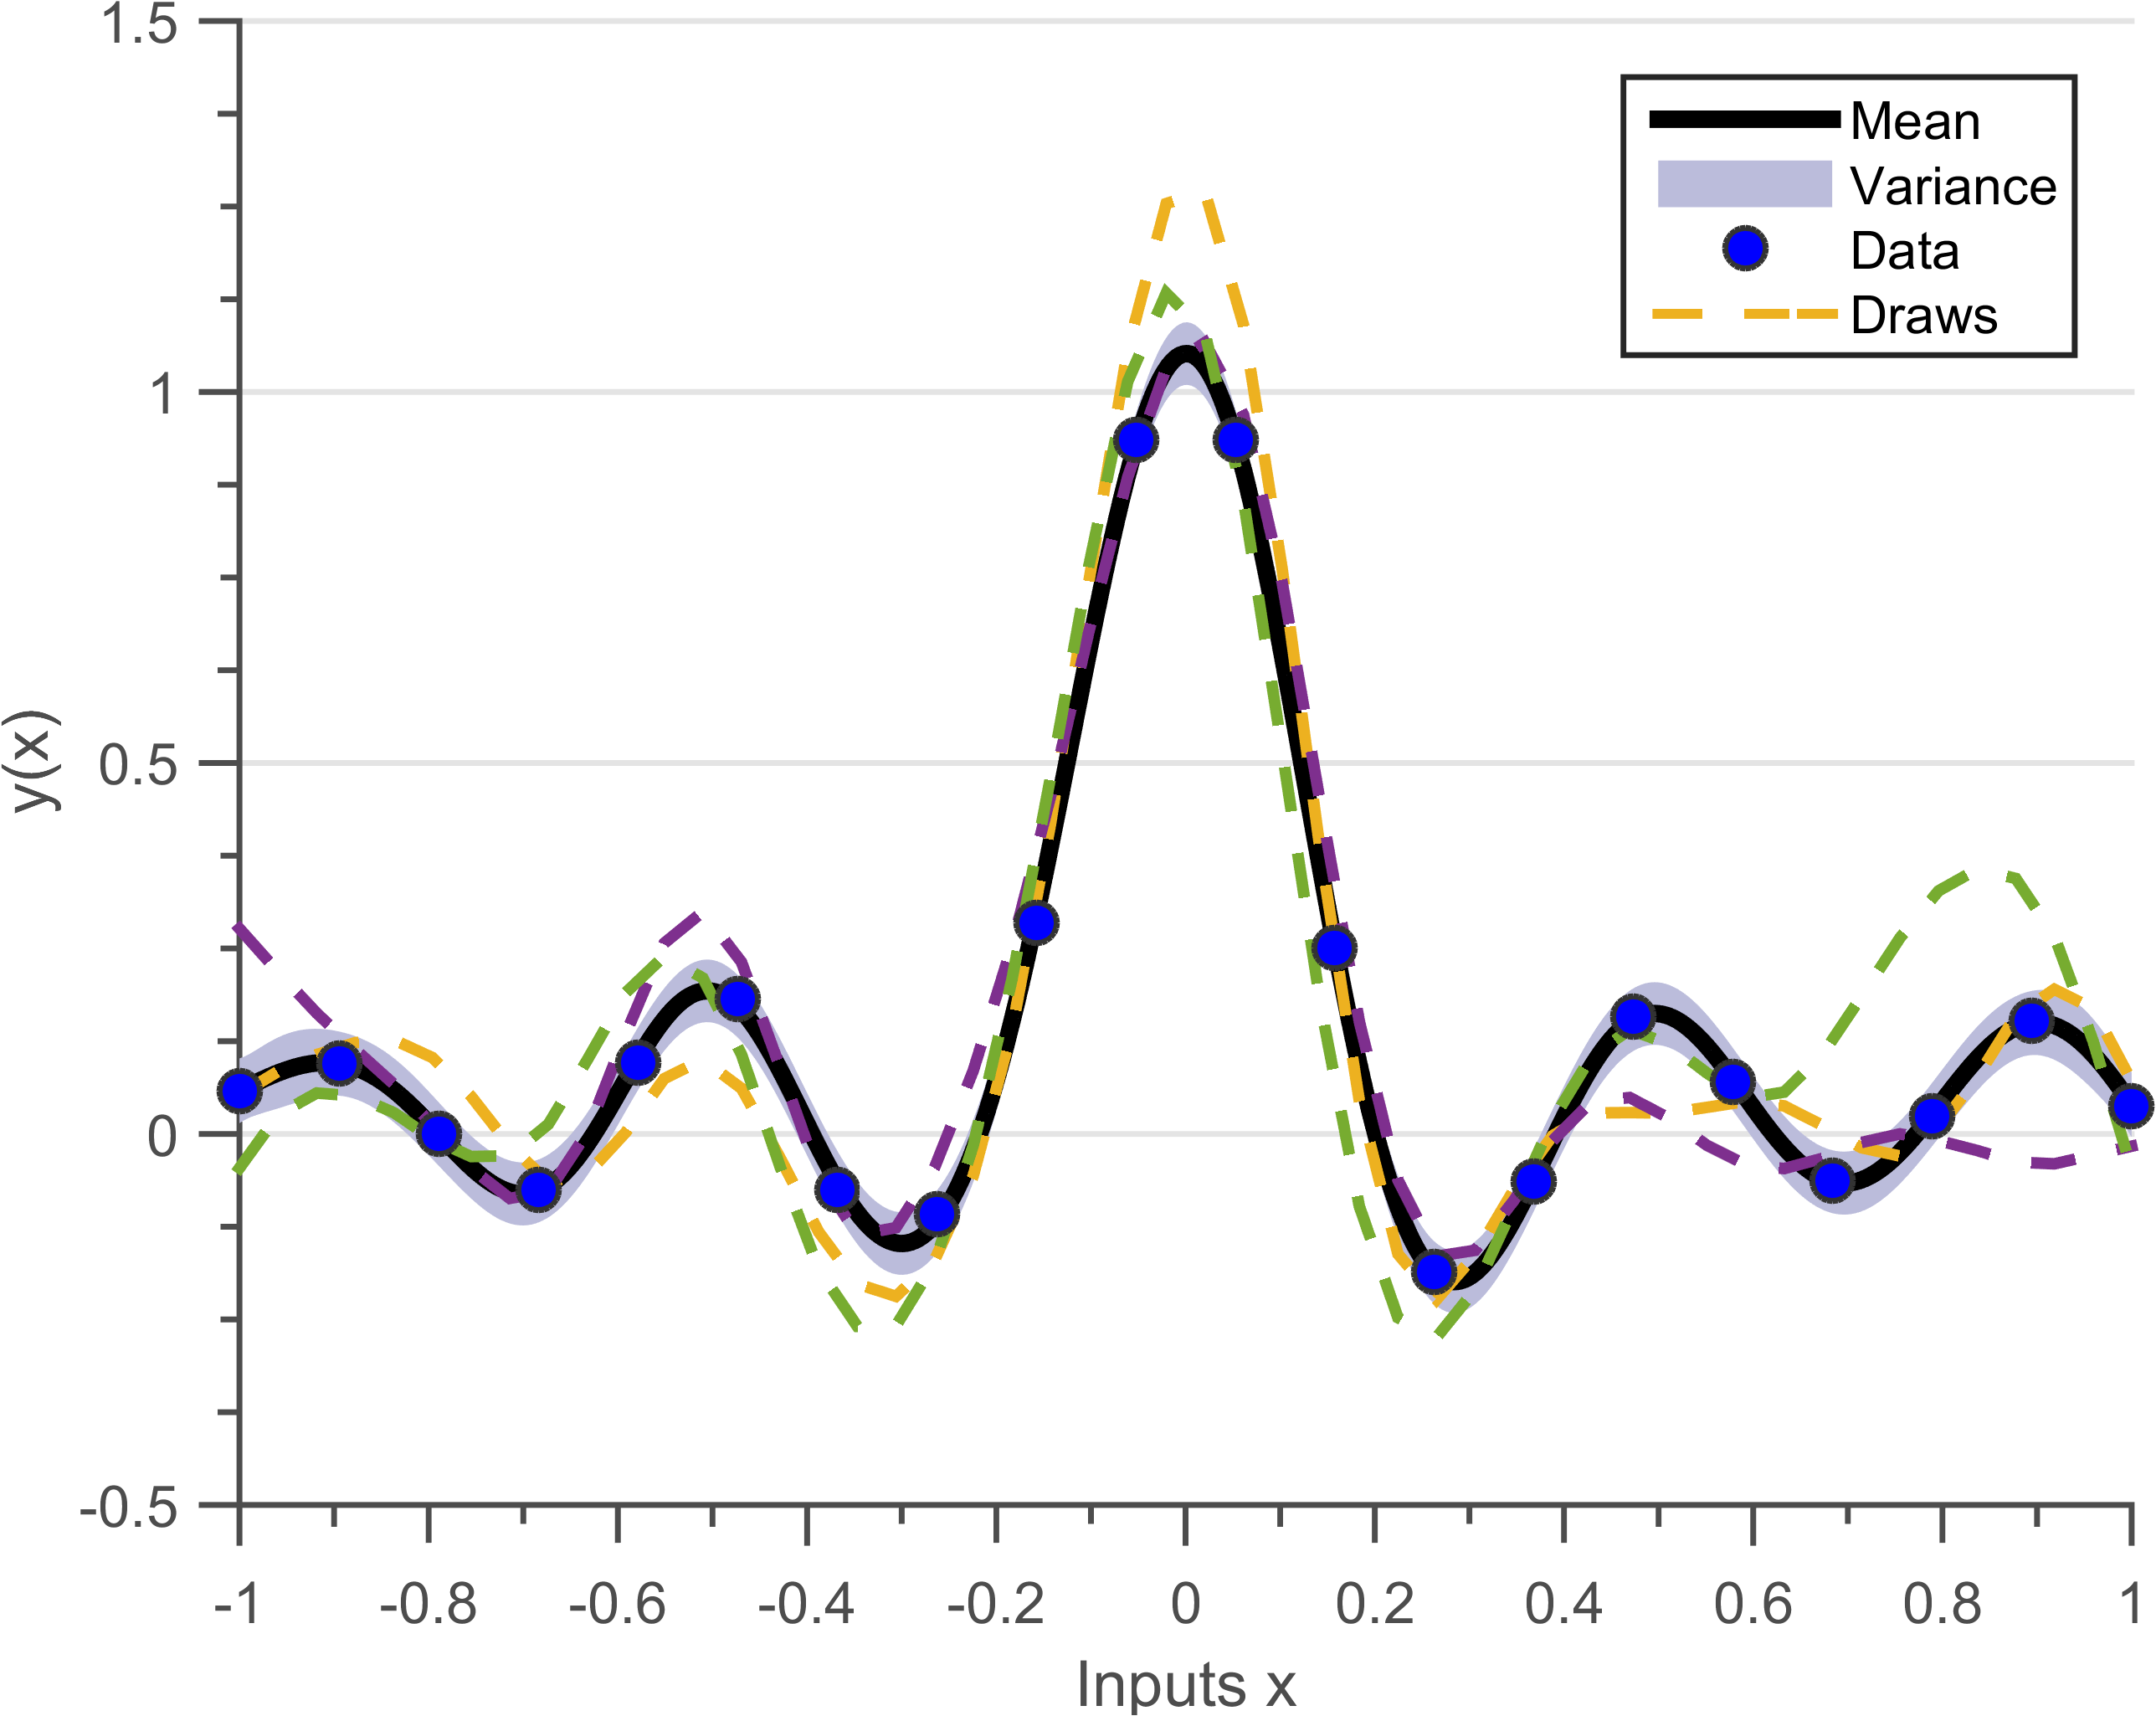
\includegraphics[width=0.29\textwidth]
        {imagesPart2/drawsOptimizedPosteriorSE}
        \label{subFigdrawsOptimizedPosteriorSE}
  }\quad
\caption{Posterior distributions from three different covariance functions after maximizing the hyper-parameters.}
       \label{figOptimizedPosteriorCh4}
\end{figure}

If nothing is known about the data or type of experiment and the number of hyper-parameters are same then the covariance function with the maximum optimized marginal likelihood should be a preferred (By this logic the SE kernel should be preferred functional form of covariance function for dataset \(\mathcal{D}_{2}\)). If number hyper-parameters are not same then marginal likelihood tends to be higher for covariance functions with greater number of hyper-parameters. \cite{duvenaud-thesis-2014, lloyd2014automatic} propose to use the Bayesian Information Criteria (equation \ref{eq:BIC}) to choose optimal covariance functions if number of hyper-parameters are not same. 

\subsection{Spectral Mixture Kernels}\label{subSecSMKernel}
Spectral mixture kernels define a more general class of stationary kernels exploiting the Bochner's theorem \cite{bochner1959lectures}. They define the power spectrum as a scale location mixture of Gaussians \cite{wilson2013gaussian}. This has two benefits firstly, with enough Gaussian components, scale location mixtures of Gaussians can approximate a curve up to arbitrary precision\cite{kostantinos2000gaussian, bishop2006pattern}. Secondly, the inverse Fourier transform of a Scale location mixture of Gaussians is analytically tractable and is also a mixture of Gaussians.

\begin{equation}\label{eqPowerSpectrumSSM}
    S_{SM}(s, \mu, \sigma, w) = \sum_{q=1}^{Q} \frac{w_{q}}{\sqrt{2\pi\sigma_{q}^2}}
\left ( \exp\left [ {-\frac{{(s-\mu_{q})^2}}{2\sigma_{q}^{2}}} \right ] + \exp\left [ {-\frac{{(-s-\mu_{q})^2}}{2\sigma_{q}^{2}}} \right ] \right  )
\end{equation}

Here, \( S_{SM}\) is the power spectrum of the spectral mixture kernel. Each Gaussian  component \(q\) has a mean \(\mu_{q}\), variance \(\sigma_{q}\) and weight \(w_{q}\) , there are total \(Q\) such components. The second term \(\exp\left [ {-\frac{{(-s-\mu_{q})^2}}{2\sigma_{q}^{2}}} \right ]\) is needed because a power spectrum of a valid kernels should be symmetric around \(s=0\). The inverse Fourier transform of such a power spectrum will be a valid kernel and can be written as below, for a detailed derivation refer to \cite{wilson2014thesis}.

\begin{equation}\label{eqCovarianceKSM}
k_{SM}(\tau, \mu, \sigma, w) = \sum_{q=1}^{Q}w_{q}cos(2\pi\mu_{q}) exp[-2\pi^{2}\tau^{2}\sigma_{q}^2]
\end{equation}

Here, \(k_{SM}\) is the covariance function of the above power spectrum (equation \ref{eqPowerSpectrumSSM}). The parameter \(w_{q}\) is the weight of the Gaussian component \(q\), the mean of the Gaussian component \(\mu_{q}\) defines the period of kernel while the variance \(\sigma_{q}\) of the Gaussian component denotes inverse of the inverse length scale . Spectral mixture kernels are easily interpretable and can be used as a replacement to many available basic kernels. They can be used to perform pattern discovery, infer negative covariances and perform extrapolation \cite{wilson2014thesis}. 

Although there do exist various other types of basic stationary kernels; for example Gibbs kernel, Rational Quadratic kernel, Periodic kernel etc we mention here only a small quantity of stationary kernels, for more detailed list please refer to work from \cite{Rasmussen2005, duvenaud2013structure, wilson2014thesis}.

Dynamic engineering systems are generally, parametrized by their modal frequencies and participation factors. In structural engineering identification of modal frequencies is an important step for certification, while minor change in modal frequencies can help in speedy discovery of failure. In the next section we apply the Spectral Mixture kernel to identify the modal frequencies of a structural system, parts of the following work have been published in \cite{chiplunkar2017operational}.

\subsection{Application: Identifying Structural Dynamics Parameters}\label{subSecSMKernelApplication}
Modal analysis has been widely used as a means of identifying dynamic properties such as modal frequencies, damping ratios and mode shapes of a structural system. Traditionally, the system is subjected to artificial input excitations and output deformations (displacements, velocities or accelerations) are measured. These later help in identifying the modal parameters of the system, this process is called Experimental Modal Analysis (EMA). 

Since the last decade Operational Modal Analysis (OMA) has gained considerable interest in the community. OMA identifies the modal parameters only from the output measurements while assuming ambient excitations as random noise. OMA is cheaper because it does not require expensive experimental setup and and can be used in real time operational use cases such as health monitoring \cite{peeters2005industrial, shahdin2010correlating, rainieri2007automated}. 

As stated earlier the operational modal analysis is an output dependent modal identification technique. The only thing required is the measurement from the accelerometers placed on the structure. Figure \ref{subfig:randomOutput} shows an example of ambient measurements \(x(t)\) on a structure.  In almost all OMA algorithms the measurement \(x(t)\) is assumed to be generated from a random force excitation. 

In the last few decades several algorithms primarily using the assumption of second order differential, Multi Degree Of Freedom (MDOF) system (equation \ref{eq:secondOrderSystem}) have been developed to find modal parameters in \cite{guillaume2003poly, richardson1982parameter}.

\begin{equation}\label{eq:secondOrderSystem}
    [M]\{\ddot{x}(t)\} + [C]\{\dot{x}(t)\} + [K]\{x(t)\} = \{f(t)\}
\end{equation}

Here, \([M]\), \([C]\) and \([K]\) denote the mass, damping and stiffness matrices respectively. While, \(\{x(t)\}\) and \(\{f(t)\}\) denote the displacement and force vectors at the time \(t\). The Natural Excitation Technique \cite{james1995natural} proves that the auto-correlation function \(k(\tau)\) can be written as sum of decaying sinusoid's \cite{spitznogle1970representation, ibrahim1977method, guillaume2003poly}. The auto-correlation describes the similarity between measurement as a function of time lag \(\tau\) between them figure \ref{subfig:autocorrelationOutput}.  

\begin{equation}\label{eq:NeXT}
    k(\tau) = \int x(t)x(t-\tau)dt \quad k(\tau) = \sum A_{i}exp(-\lambda_{i}\tau)sin(B_{i}\tau)
\end{equation}

Here, \(k(\tau)\) denotes the auto-correlation for random vector \(x(t)\) as a function of time lag \(\tau\). Here, \(\lambda_{i}\) and \(A_{i}\) denotes the modal frequency and mode shapes for the \(i^{th}\) mode. The above coefficients are found by minimizing the least square error between the measured \(k(\tau)\) and the predicted \(k(\tau)\) from equation \ref{eq:NeXT}

If we assume the measurement \(x(t)\) to be a stationary random process, then according to Bochner's theorem the Fourier transform of \(k(\tau)\) (power spectrum \(S(s)\)) exists \cite{bochner2016lectures}. Figure \ref{subfig:psdOutput} shows the power spectrum calculated for the measurement \(x(t)\) shown in figure \ref{subfig:randomOutput}. Using the above mentioned second order differential equation assumption a Rational Fractional Polynomial (equation \ref{eq:RFP}) can be used to fit a power spectrum \cite{richardson1982parameter, allemang1998unified, chauhan2007unified}.

\begin{equation}\label{eq:RFP}
S(s) = \int k(\tau) e^{-2 \pi is^{T} s}d\tau \quad    S(s) = \frac{\sum a_{k}(s)^{k}}{\sum b_{l}(s)^{l}}
\end{equation}

Here, the poles of the polynomial denote the modal frequencies, while other modal parameters can be derived from the coefficients \(a_{k}\) and \(b_{l}\). The coefficients of the polynomial can be found by minimizing the least squared error. RFP based algorithms face problems since as the number of modes increase the matrix becomes ill-conditioned which gives rise to stability issues in prediction of modal parameters. In the next section we will drop the assumption of second order differential system and treat the modal identification as a purely curve-fitting problem.

Two of the above mentioned OMA algorithms ``Natural Excitation Technique" in the time lag (\( \tau\))domain and ``Rational Fractional Polynomial" in the frequency domain \(s\), have a core assumption of second order differential system. This assumption fails for non-linear systems and for cases where modal frequencies are very close. Instead we propose the spectral mixture kernel to fit the measurement \(x(t)\). 

Using the same hypothesis used in section \ref{subSecSMKernel}, we can say that a scale-location mixture of Gaussian components can approximate any distribution. We thus place a Gaussian Mixture Model (GMM) on the power spectrum (\(S(s)\)), this means that we are assuming a prior distribution of \(x(t)\) as a Gaussian Process with a Spectral Mixture kernel (equation \ref{eqTimeFitting}). The hyper-parameters of the system are: the mean \(\mu_{q}\) defines the modal frequency, the variance \(\sigma_{q}\) which is a measure of damping, the weight \(w_{q}\) which defines the participation factor of component \(q\) and the total number of components \(Q\).

\begin{equation}\label{eqTimeFitting}
\Pr[x(t)] = GP(0, k_{SM} = \sum_{q=1}^{Q}w_{q}cos(2\pi\mu_{q}) exp[-2\pi^{2}\tau^{2}\sigma_{q}^2)
\end{equation}

We would like to emphasize that keeping the computational complexities aside, fitting a Spectral Mixture GP in time-domain equation \ref{eqTimeFitting}, fitting equation \ref{eqCovarianceKSM} for covariance identification and fitting a GMM equation \ref{eqPowerSpectrumSSM} in the frequency-domain are equivalent. In the publication \cite{chiplunkar2017operational} we fit a GMM on the frequency domain, here we propose to fit the GP on the measurements \(x(t)\) . Refer to table \ref{tab:comparisonOfFittingFunctions} for a more comprehensive view at various fitting functions.

\begin{figure*}[!ht]
  \centering
  \subfigure[Measured output on accelerometers \(x(t)\)]
  {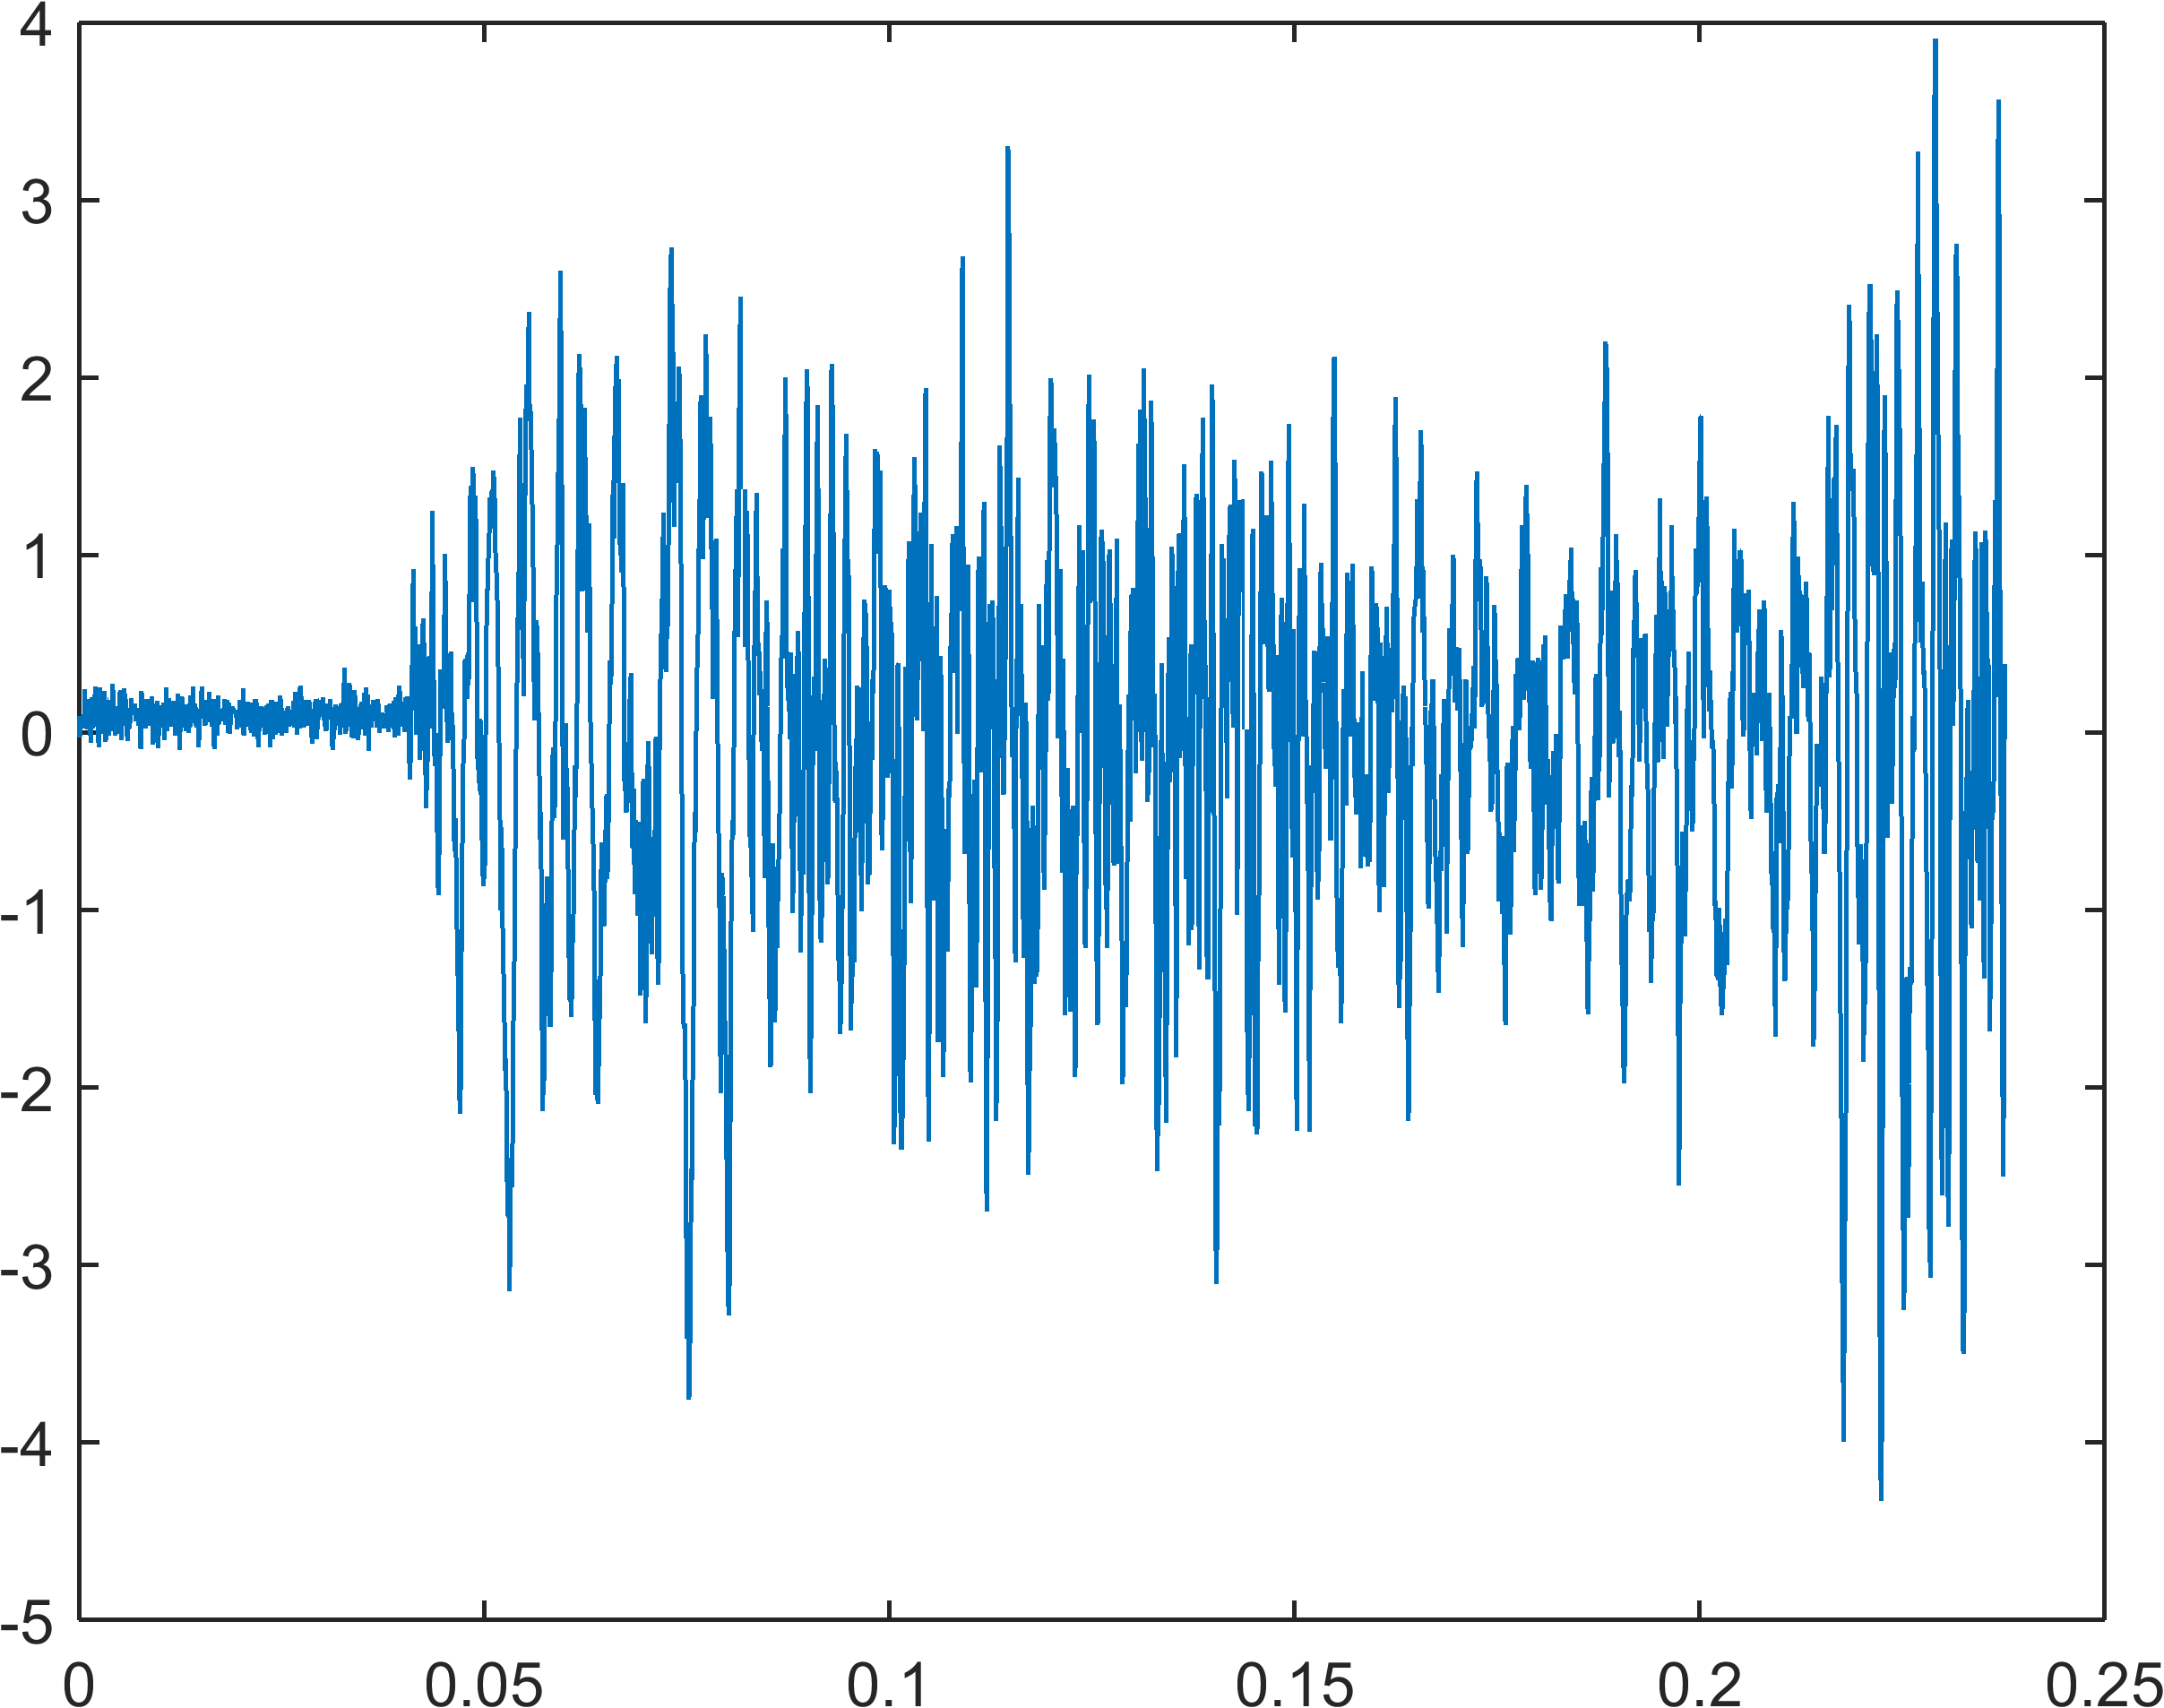
\includegraphics[width=0.3\textwidth]{imagesPart2/randomOutput}\label{subfig:randomOutput}}\quad
  \subfigure[Auto-correlation \(k(\tau)\) of the measured output fig: \ref{subfig:randomOutput}]
  {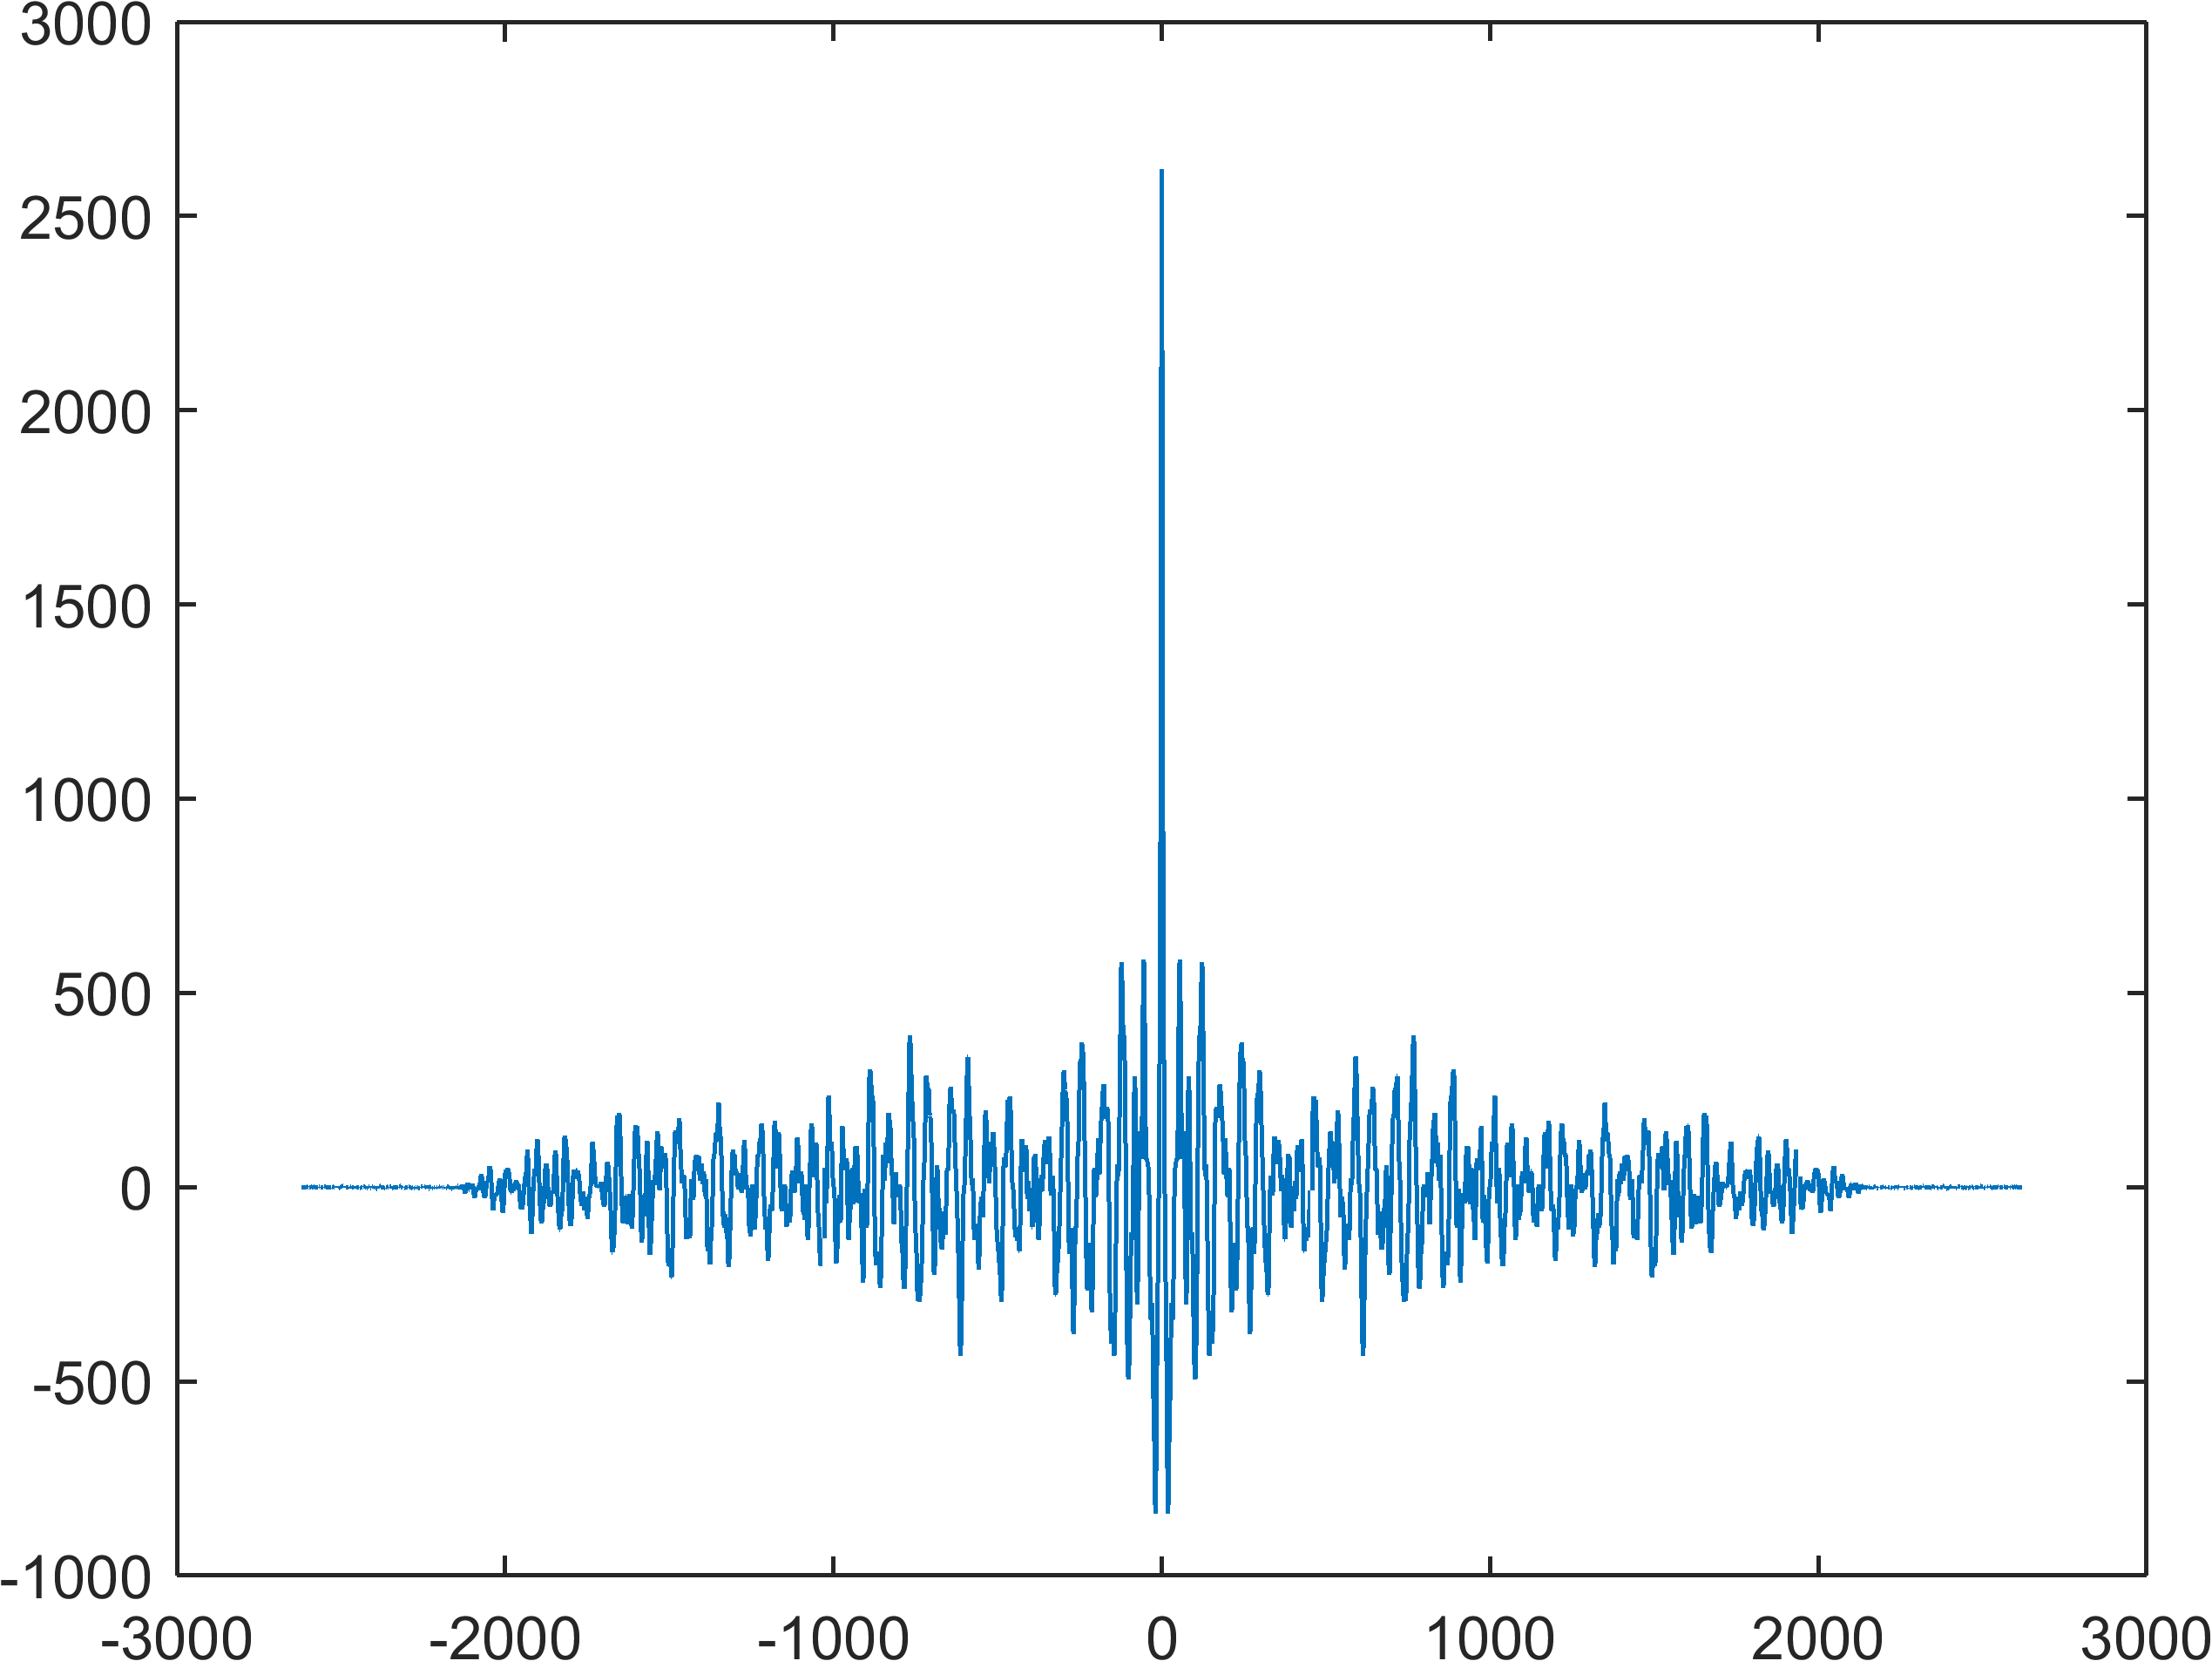
\includegraphics[width=0.3\textwidth]{imagesPart2/autocorrelationOutput}\label{subfig:autocorrelationOutput}}\quad
  \subfigure[Power spectrum density \(S(s)\) of the output fig: \ref{subfig:randomOutput}]
  {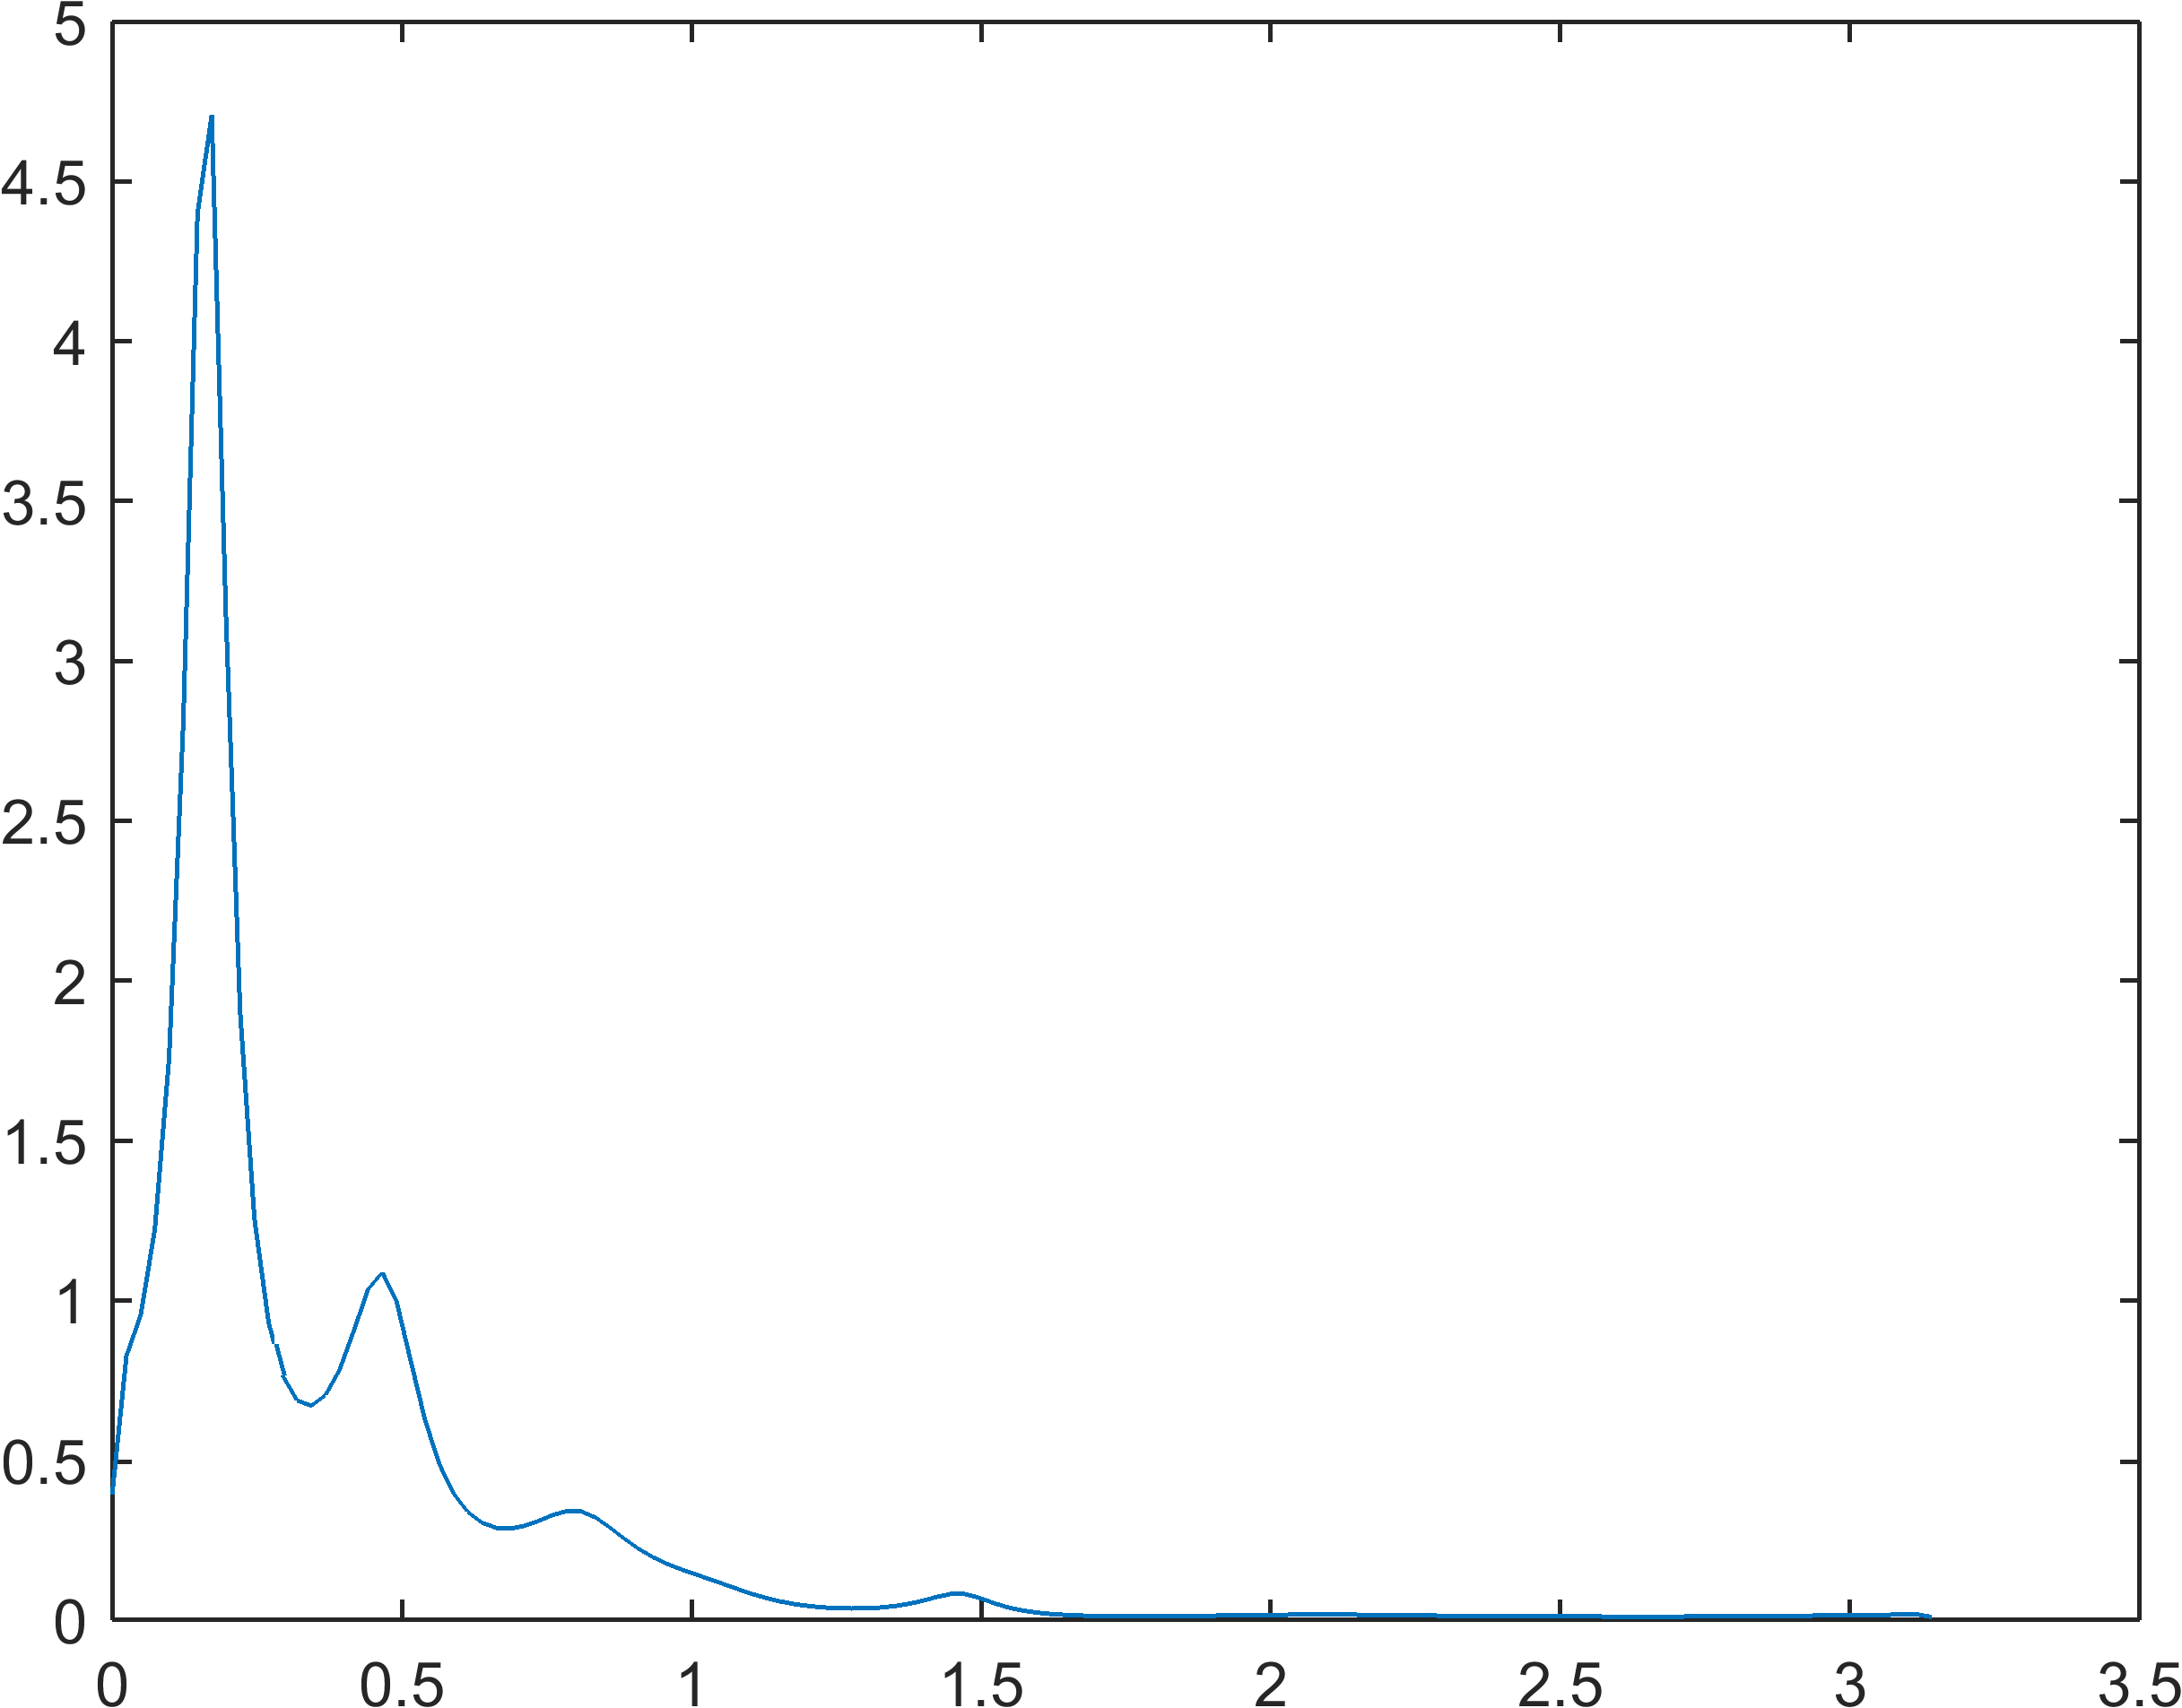
\includegraphics[width=0.3\textwidth]{imagesPart2/psdOutput}\label{subfig:psdOutput}}
  
  \caption{Different types of measurements for estimation of Modal parameters in OMA}
\end{figure*}

\renewcommand{\arraystretch}{1.2}
\begin{table}[!h]
    \centering
\begin{tabularx}{0.915\textwidth}{c|c|c}
  \hline
  Measurement & Auto-correlation & Power Spectrum \\
  \hline
  $x(t)$ & $k(\tau) = \int x(t)x(t-\tau)dt$ &  $S(s) = \int k(\tau)exp(-2 \pi i s^{T} \tau )d\tau$\\
  \hline \hline
  \multicolumn{3}{|c|}{Assumption: Second Order Differential}\\
  \hline
   & $ \sum A_{i}exp(-\lambda_{i}\tau)sin(B_{i}\tau)$ & $\frac{\sum a_{k}(s)^{k}}{\sum b_{l}(s)^{l}}$\\
   \hline \hline
   \multicolumn{3}{|c|}{Assumption: Gaussian Mixture Model}\\
   \hline
   $GP(0 , k_{SM})$ 
   & $  \sum w_{i} cos(2\pi\mu_{i}\tau) exp\{-2\pi^{2}\sigma_{i}^{2}\tau^{2}\}$ 
   & $ \sum w_{i}  \frac{1}{\sqrt{2\pi\sigma_{i}^{2}}}exp\{\frac{1}{2\sigma_{i}^{2}}(s-\mu_{i})^{2}\} $\\
   \hline
\end{tabularx}
\caption{Comparison of fitting functions}
  \label{tab:comparisonOfFittingFunctions}
\end{table}

While the modal parameters can be chosen by minimizing the least square error, how to choose the number of modes is a recurring question in several OMA algorithms. This problem is partially resolved by using stabilization diagrams or mode identification functions \cite{allemang1998unified, williams1985multivariate, shih1988complex}. But in practical situations engineering judgment is often required to estimate the optimal modal order. To automatically choose \(Q\), we use the Bayesian Information Criteria (BIC) \cite{findley1991counterexamples} which penalizes more complex models to estimate the parameter \(Q\). The BIC estimate has been earlier used to find the optimal functional form of covariance function \cite{duvenaud2013structure}

\textbf{\begin{equation}\label{eq:BIC}
    BIC(Q) = N\ln(ML) + N_{hyp}\ln(N)
\end{equation}}

Here, \(n\) denotes the number of data-points to fit, \(ML\) denotes the marginal likelihood of the fit and \(N_{hyp}\) denote the number of hyper-parameters to fit. The BIC performs a trade-off between the data-fit term \(N\ln(ML)\) and the complexity penalty term \(N_{hyp}\ln(N)\), basically penalizing for over-fitting. Lowest value of BIC is preferred. 

\textbf{Define an algorithm here on how to find the Q etc}

Generally, identification of modal frequencies requires engineering judgment, i.e. engineers have to look at the stabilization diagrams and figure out the optimal value of modal order. Using the Spectral mixture kernel we have encoded the knowledge of peaks in the power spectrum which in combination with BIC has eliminated the need to perform costly engineering judgment exercises and made the process automatic. We now compare the accuracy of finding modal frequencies using a spectral mixture kernel of NeXT methodology for a toy-dataset, and then later for a real dataset of HTC building \cite{brincker2000modal}.

\subsubsection{Results on a toy data-set}
In this section we conduct experiments, applying our approach on a highly damped 3 degree of freedom system\footnote{Dataset is available at github link: here}. As stated earlier we fit a GP model having zero mean and spectral mixture covariance on the measurements \(x(t)\) for varying number of Gaussian components \(Q\). We then evaluate the Bayesian Information Criteria to find the optimal value of \(Q\) for this measurement. The results of automatic identification are then compared to that of NeXT identification method. 

All experiments were performed on an Intel quad-core processor with 4Gb RAM. The Spectral Mixture technique suffers from multiple minimas and thus care should be taken while initializing the hyper-parameters\footnote{We first fit a Gaussian Mixture model on the power spectrum to initialize the hyper-parameters and then optimize the marginal likelihood for speedy optimization.}.  

Table \ref{tabComparisonOfModalFrequenciesToyData} shows the comparison of frequencies for Modal frequencies predicted using NeXT algorithm and Spectral Mixture algorithm. We can observe that the NeXT method cannot predict the third frequency with enough accuracy. 

\renewcommand{\arraystretch}{1}
\begin{table}[!h]
    \centering
\begin{tabular}{|l|l|l|l|}
  \hline
   & Real Frequency & NeXT Frequency & Spectral Mixture\\
  \hline 
  \hline
First Frequency (Hz) & 17.5 & 17.88 & 17.55\\
Second Frequency (Hz)  & 30 & 28.97 & 28.75\\
Third Frequency (Hz) & 35 & 39.32 & 36.80\\
   \hline
\end{tabular}
\caption{Comparison of Modal frequencies for toy data-set}
  \label{tabComparisonOfModalFrequenciesToyData}
\end{table}

Figure \ref{subfig:stabilizationDiagram} shows the stabilization diagram with increasing number of gaussians $Q$. The number of modal frequencies is dependent on the number of Gaussian components (\(Q\)), since each component will have only one mean value. As we progressively increase the number of components we start getting more and more modal frequencies. We call a frequency as stabilized if the difference between modal frequencies of two subsequent \(Q\) is less than \(1\%\), the green points are stabilized frequencies. The, figure \ref{subfig:bicVsQ} shows the BIC criterion with increasing number of Gaussian's $Q$. We can see that that the BIC is minimum for $Q=6$ and hence if we add anymore Gaussians for our dataset we will be over-fitting. The red line in figure \ref{subfig:stabilizationDiagram} shows the modal frequency with minimum BIC and hence the results of prediction.

\begin{figure*}[!ht]
  \centering
  \subfigure[Stabilization diagram with increasing number of gaussians $Q$, the dots denote the stabilized frequencies. We can observe that as the number of $Q$ increases the algorithm starts finding better and better modes.]
  {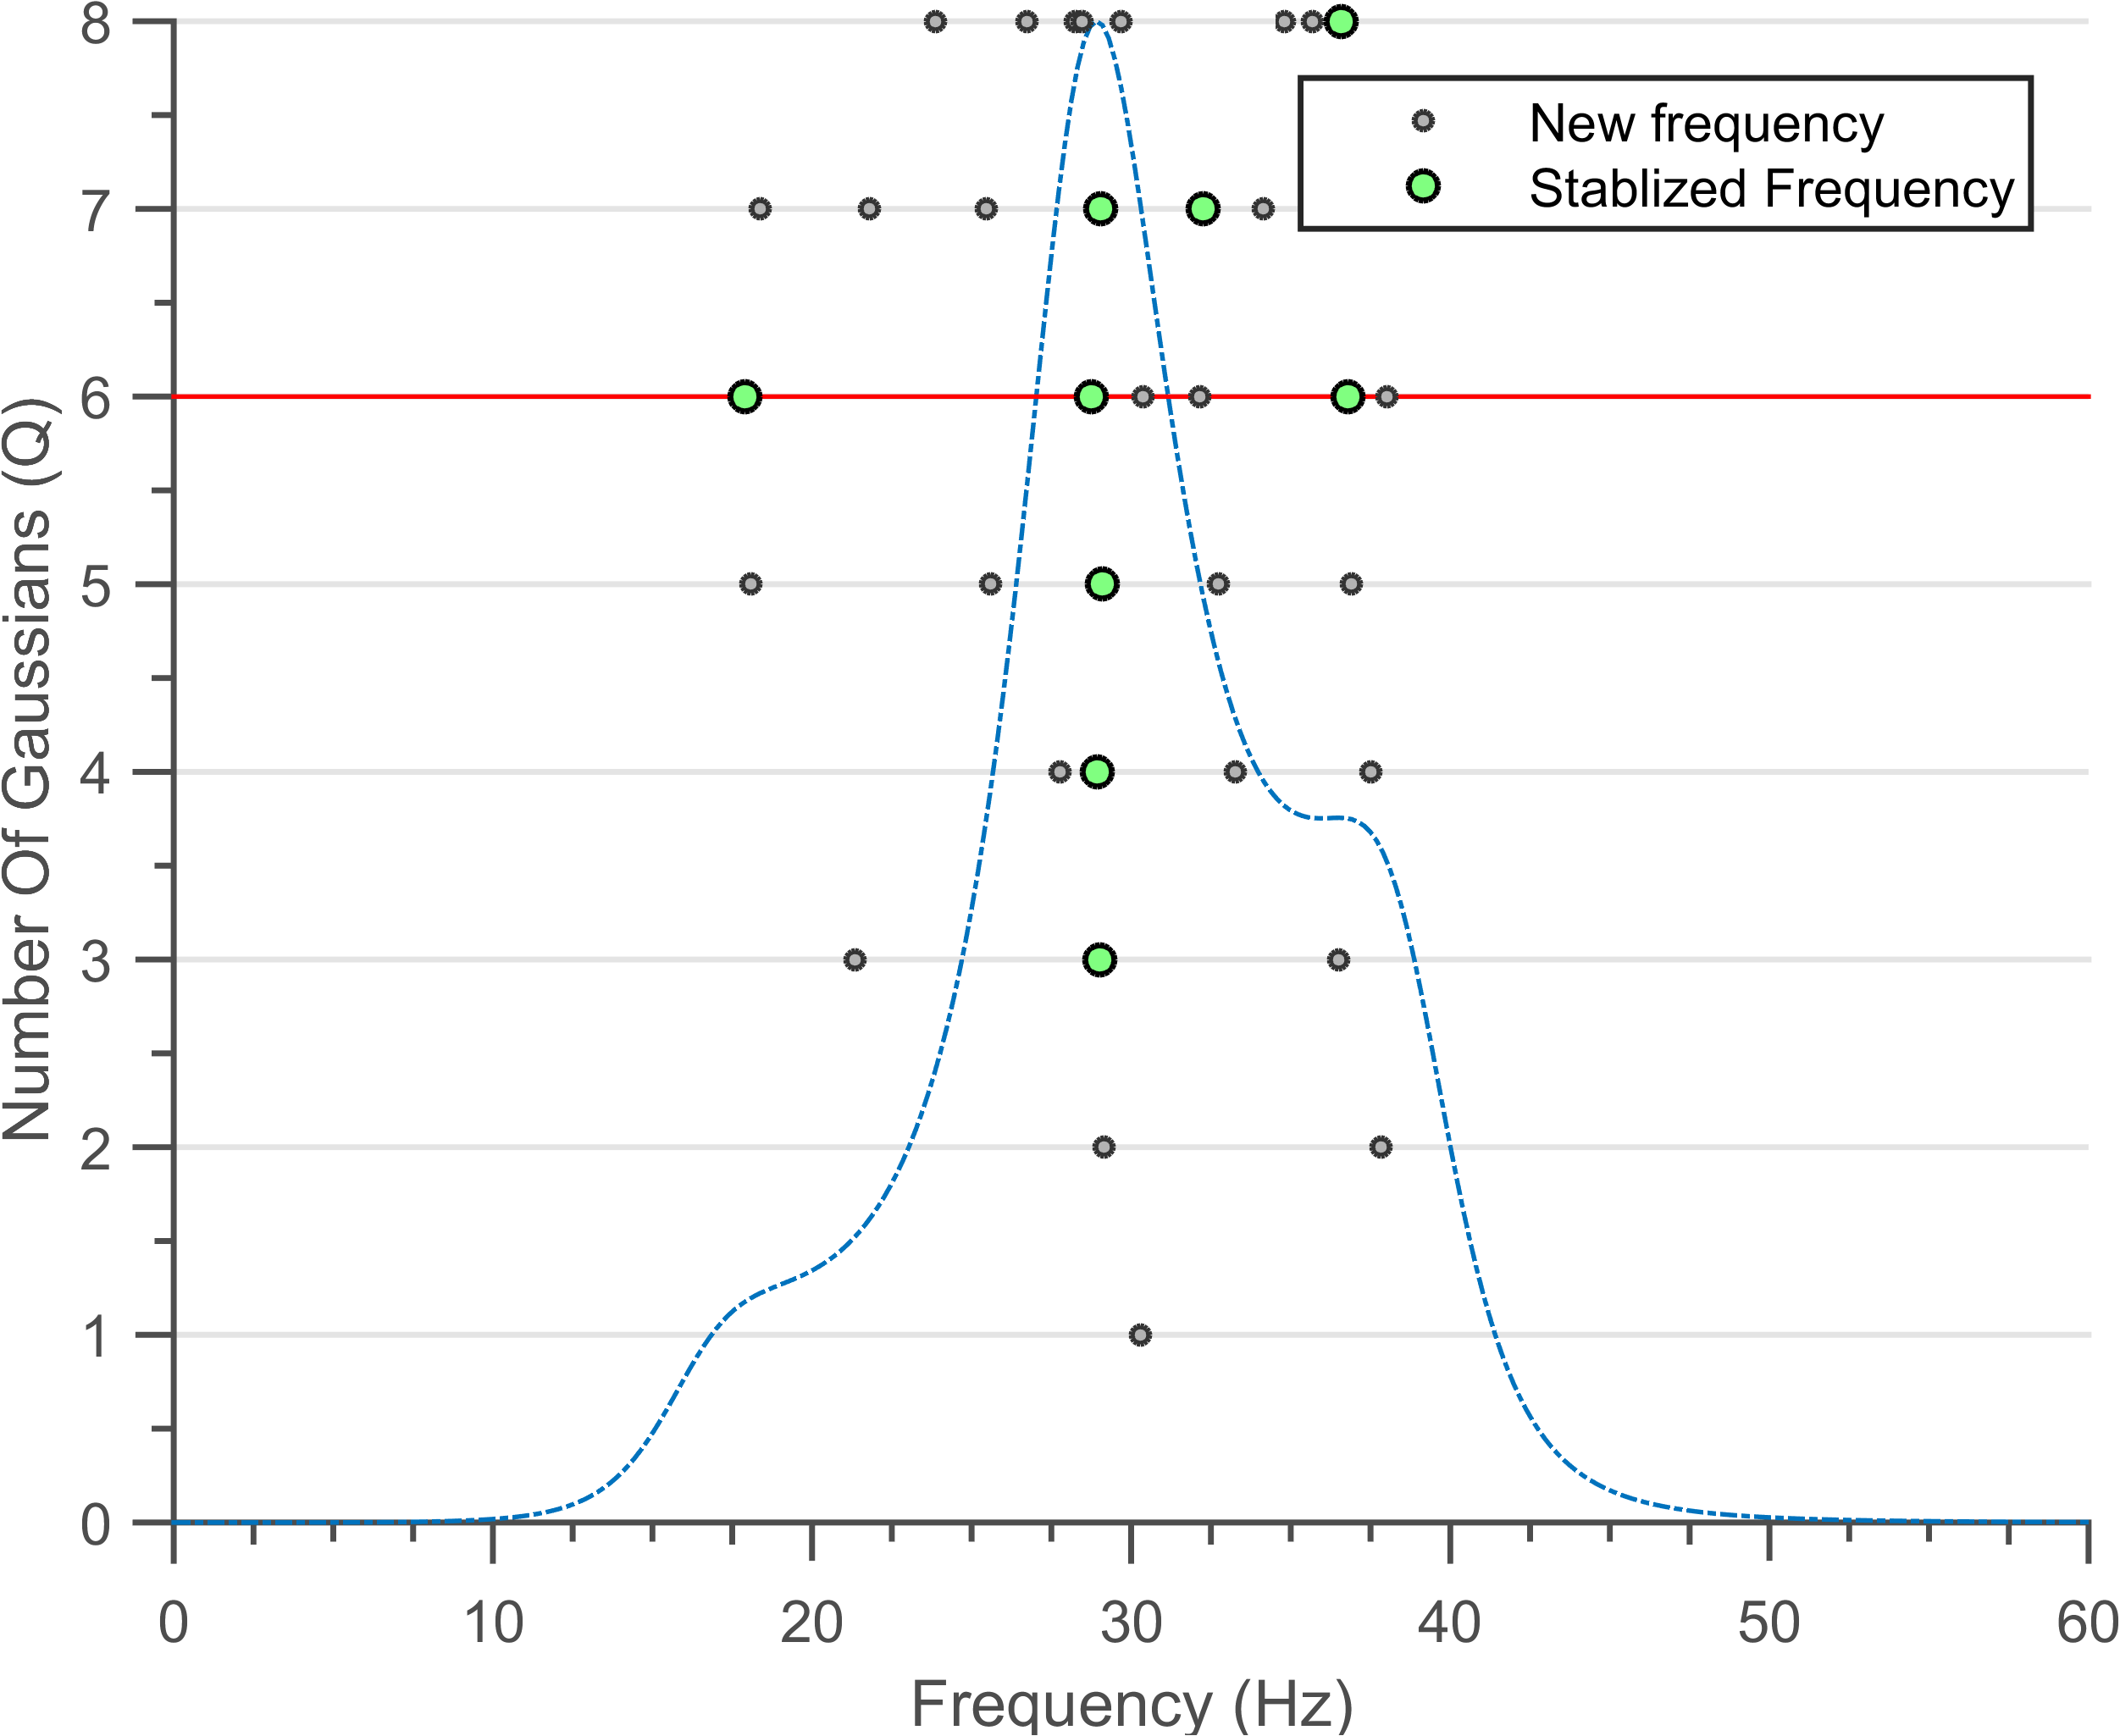
\includegraphics[width=0.45\textwidth]{imagesPart2/stabilizationDiagram_toyData}\label{subfig:stabilizationDiagram}}\quad
    \subfigure[The BIC criterion with increasing number of gaussian's $Q$. We can see that that the BIC is minimum for $Q=6$ and hence if we add anymore gaussian's for our dataset we will be performing over-fitting]
  {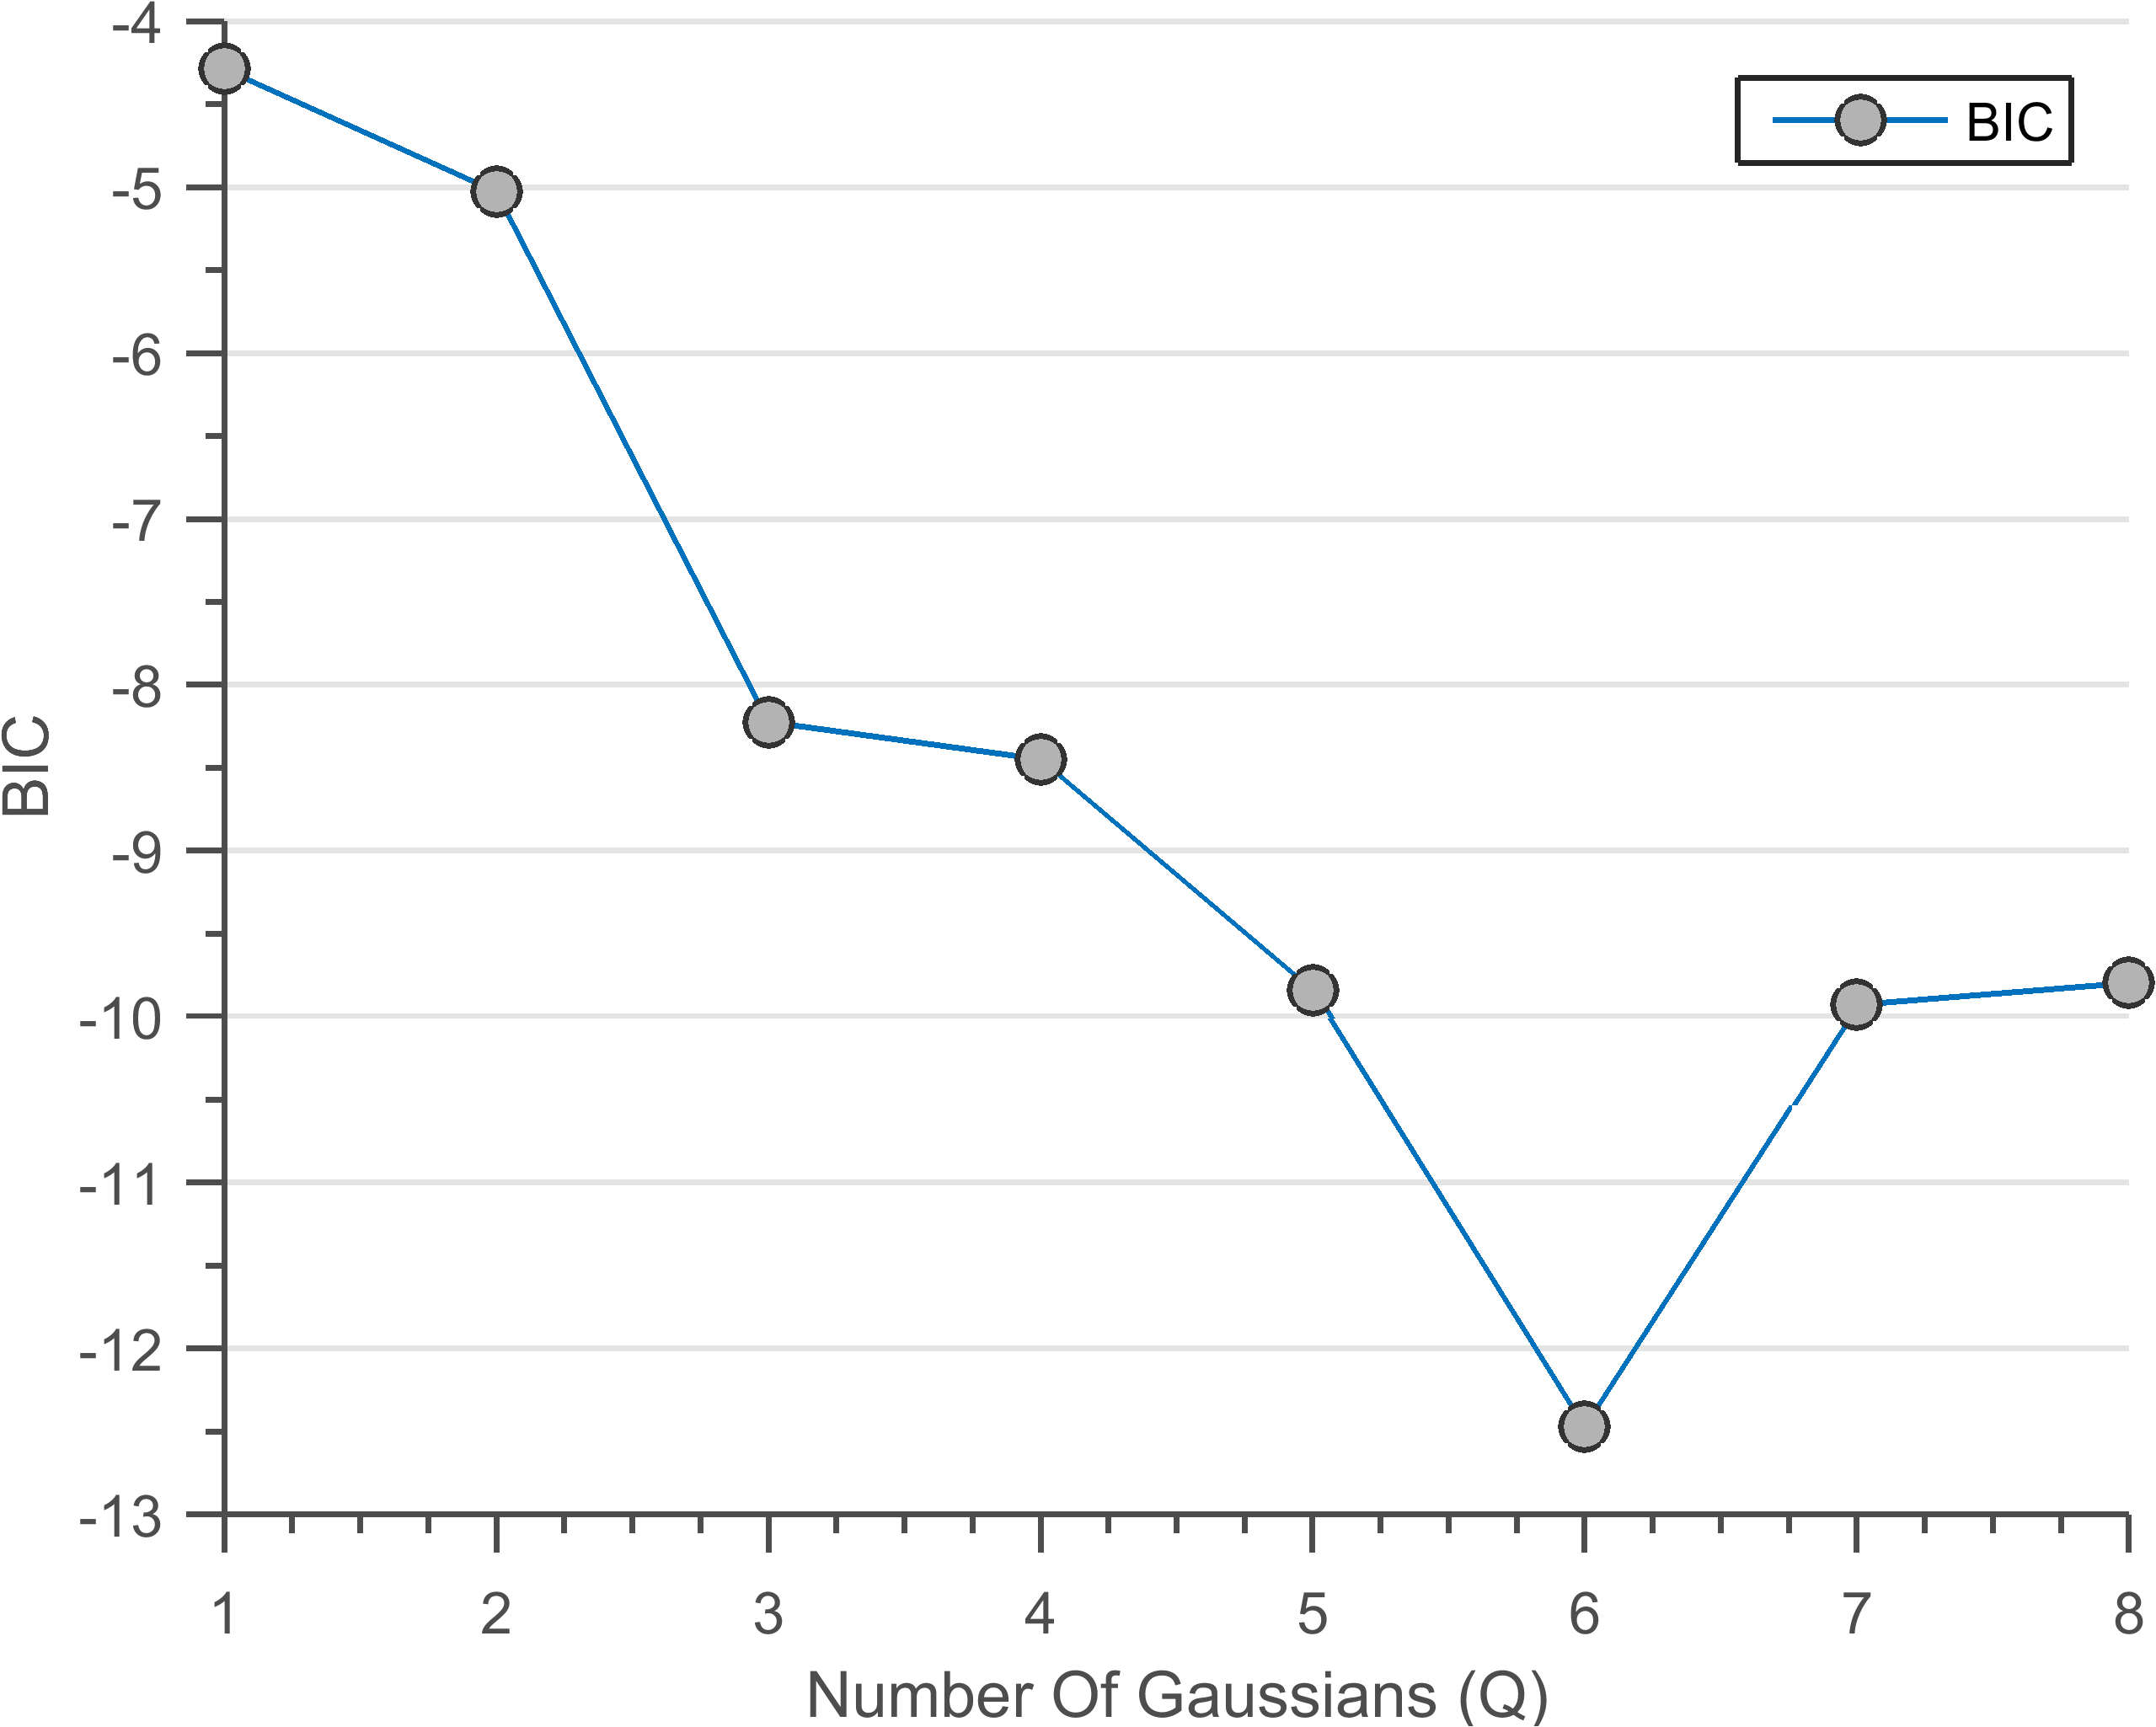
\includegraphics[width=0.45\textwidth]{imagesPart2/bicVsQ}\label{subfig:bicVsQ}}\quad
  
  \caption{Results of spectral mixture kernels on a toy dataset}
\end{figure*}

\subsubsection{Results on a HTC building dataset}
We now compare the predictions of the models on an ambient response of Heritage Court Building\footnote{The data is available at : http://www.brinckerdynamics.com/oma-toolbox}. The responses are measured at 6 different points on the building resulting in 6 different power spectrums. 

We compare the modal frequencies obtained using Spectral Mixture kernel with the modal frequencies obtained in the original paper \cite{brincker2000modal}. To compare the performance we automatically identify modal frequencies present in each of the 6 power spectrums and take the mean of the stabilized frequencies.

Table \ref{tabComparisonOfModalFrequenciesToyData} shows the comparison of Modal frequencies predicted in \cite{brincker2000modal} with Spectral Mixture algorithm. The results of the two methods are very similar, although the frequencies obtained by spectral mixture GP are completely automatic. 

\renewcommand{\arraystretch}{1}
\begin{table}[!h]
    \centering
\begin{tabular}{|l|l|l|}
  \hline
    & Spectral Mixture & \cite{brincker2000modal} \\
  \hline 
  \hline
First Frequency (Hz) & 1.23 & 1.23\\
Second Frequency (Hz)  & 1.29 & 1.27\\
Third Frequency (Hz) & 1.43 & 1.45\\
Fourth Frequency (Hz) & 3.87 & 3.86\\
Fifth Frequency (Hz) & 4.28 & 4.25\\
   \hline
\end{tabular}
\caption{Comparison of Modal frequencies for HTC data-set}
  \label{tabComparisonOfModalFrequenciesHTCData}
\end{table}

\begin{figure*}[!ht]
  \centering
  \subfigure[Stabilization diagram for one of the 6 power spectrums. The green dots denote the stabilized frequencies, the red line is denotes minimum BIC. We can observe that as the number of $Q$ increases the algorithm starts finding better and better modes.]
  {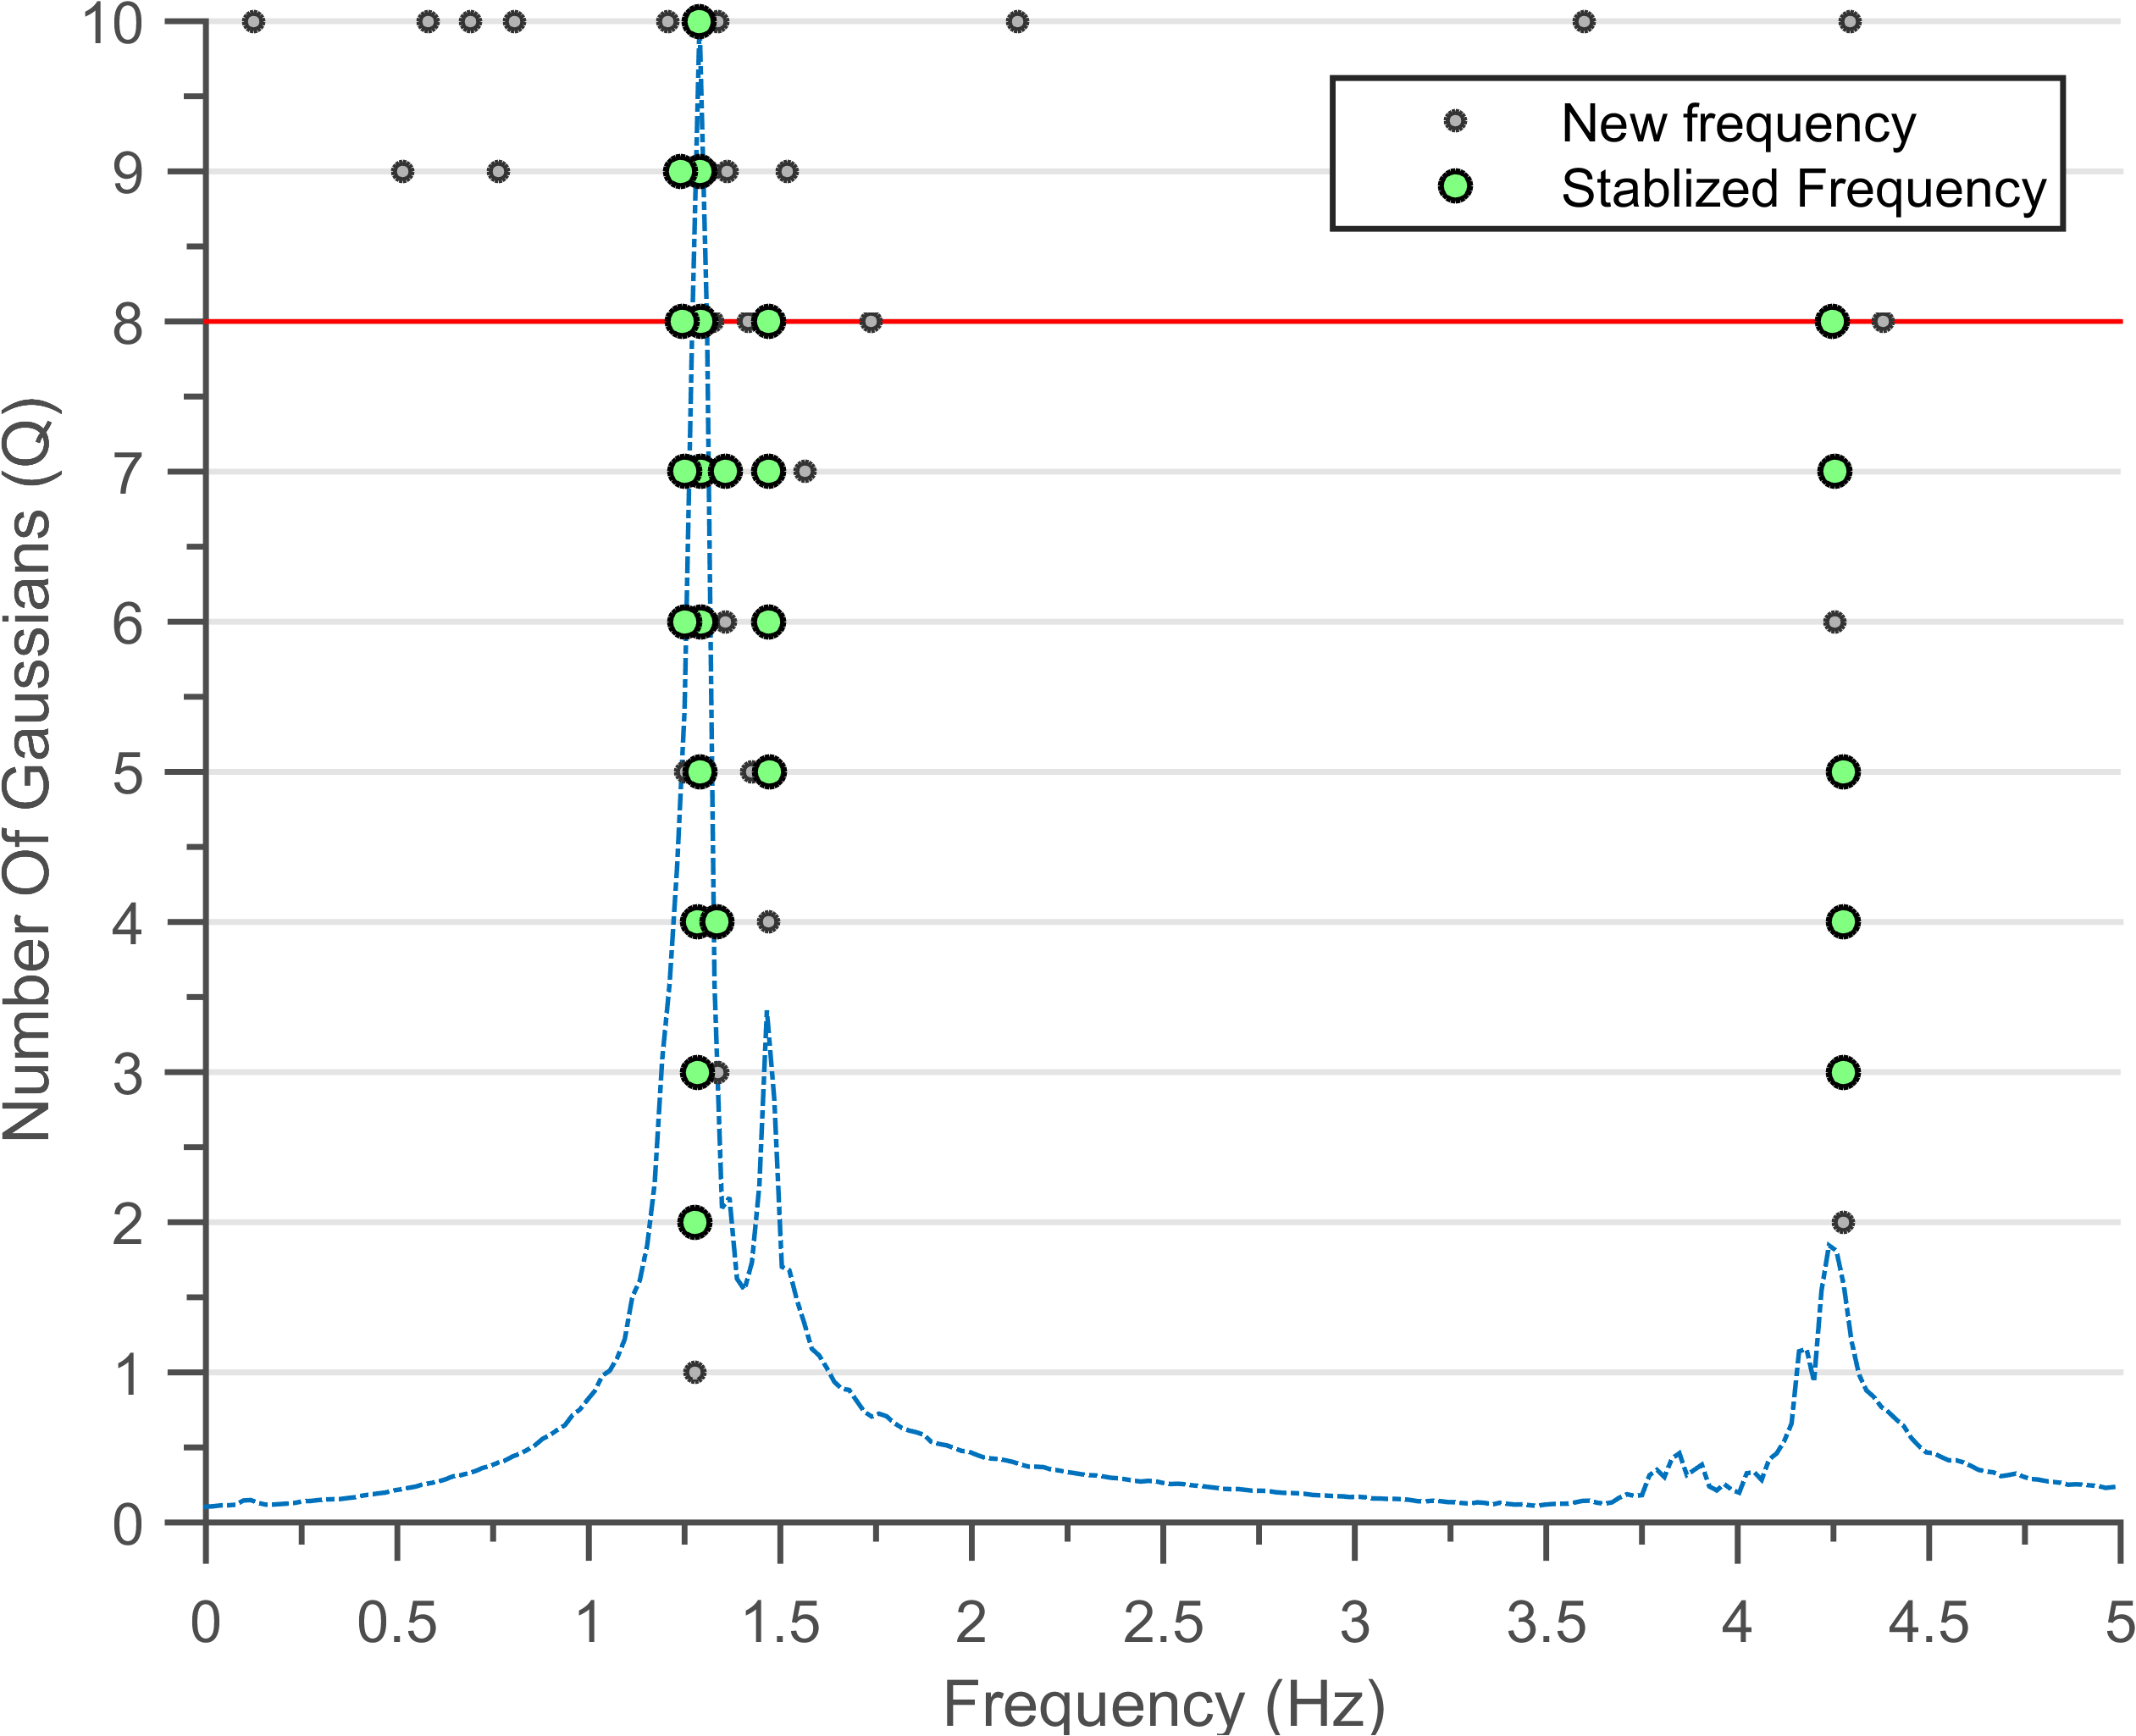
\includegraphics[width=0.45\textwidth]{imagesPart2/stabilizationDiagram_HTCBuildingData}\label{subfigStablizationHTCData}}\quad
    \subfigure[The BIC criterion with increasing number of gaussian's $Q$. We can see that that the BIC is minimum for $Q=8$ and hence if we add anymore gaussian's for our dataset we will be performing over-fitting]
  {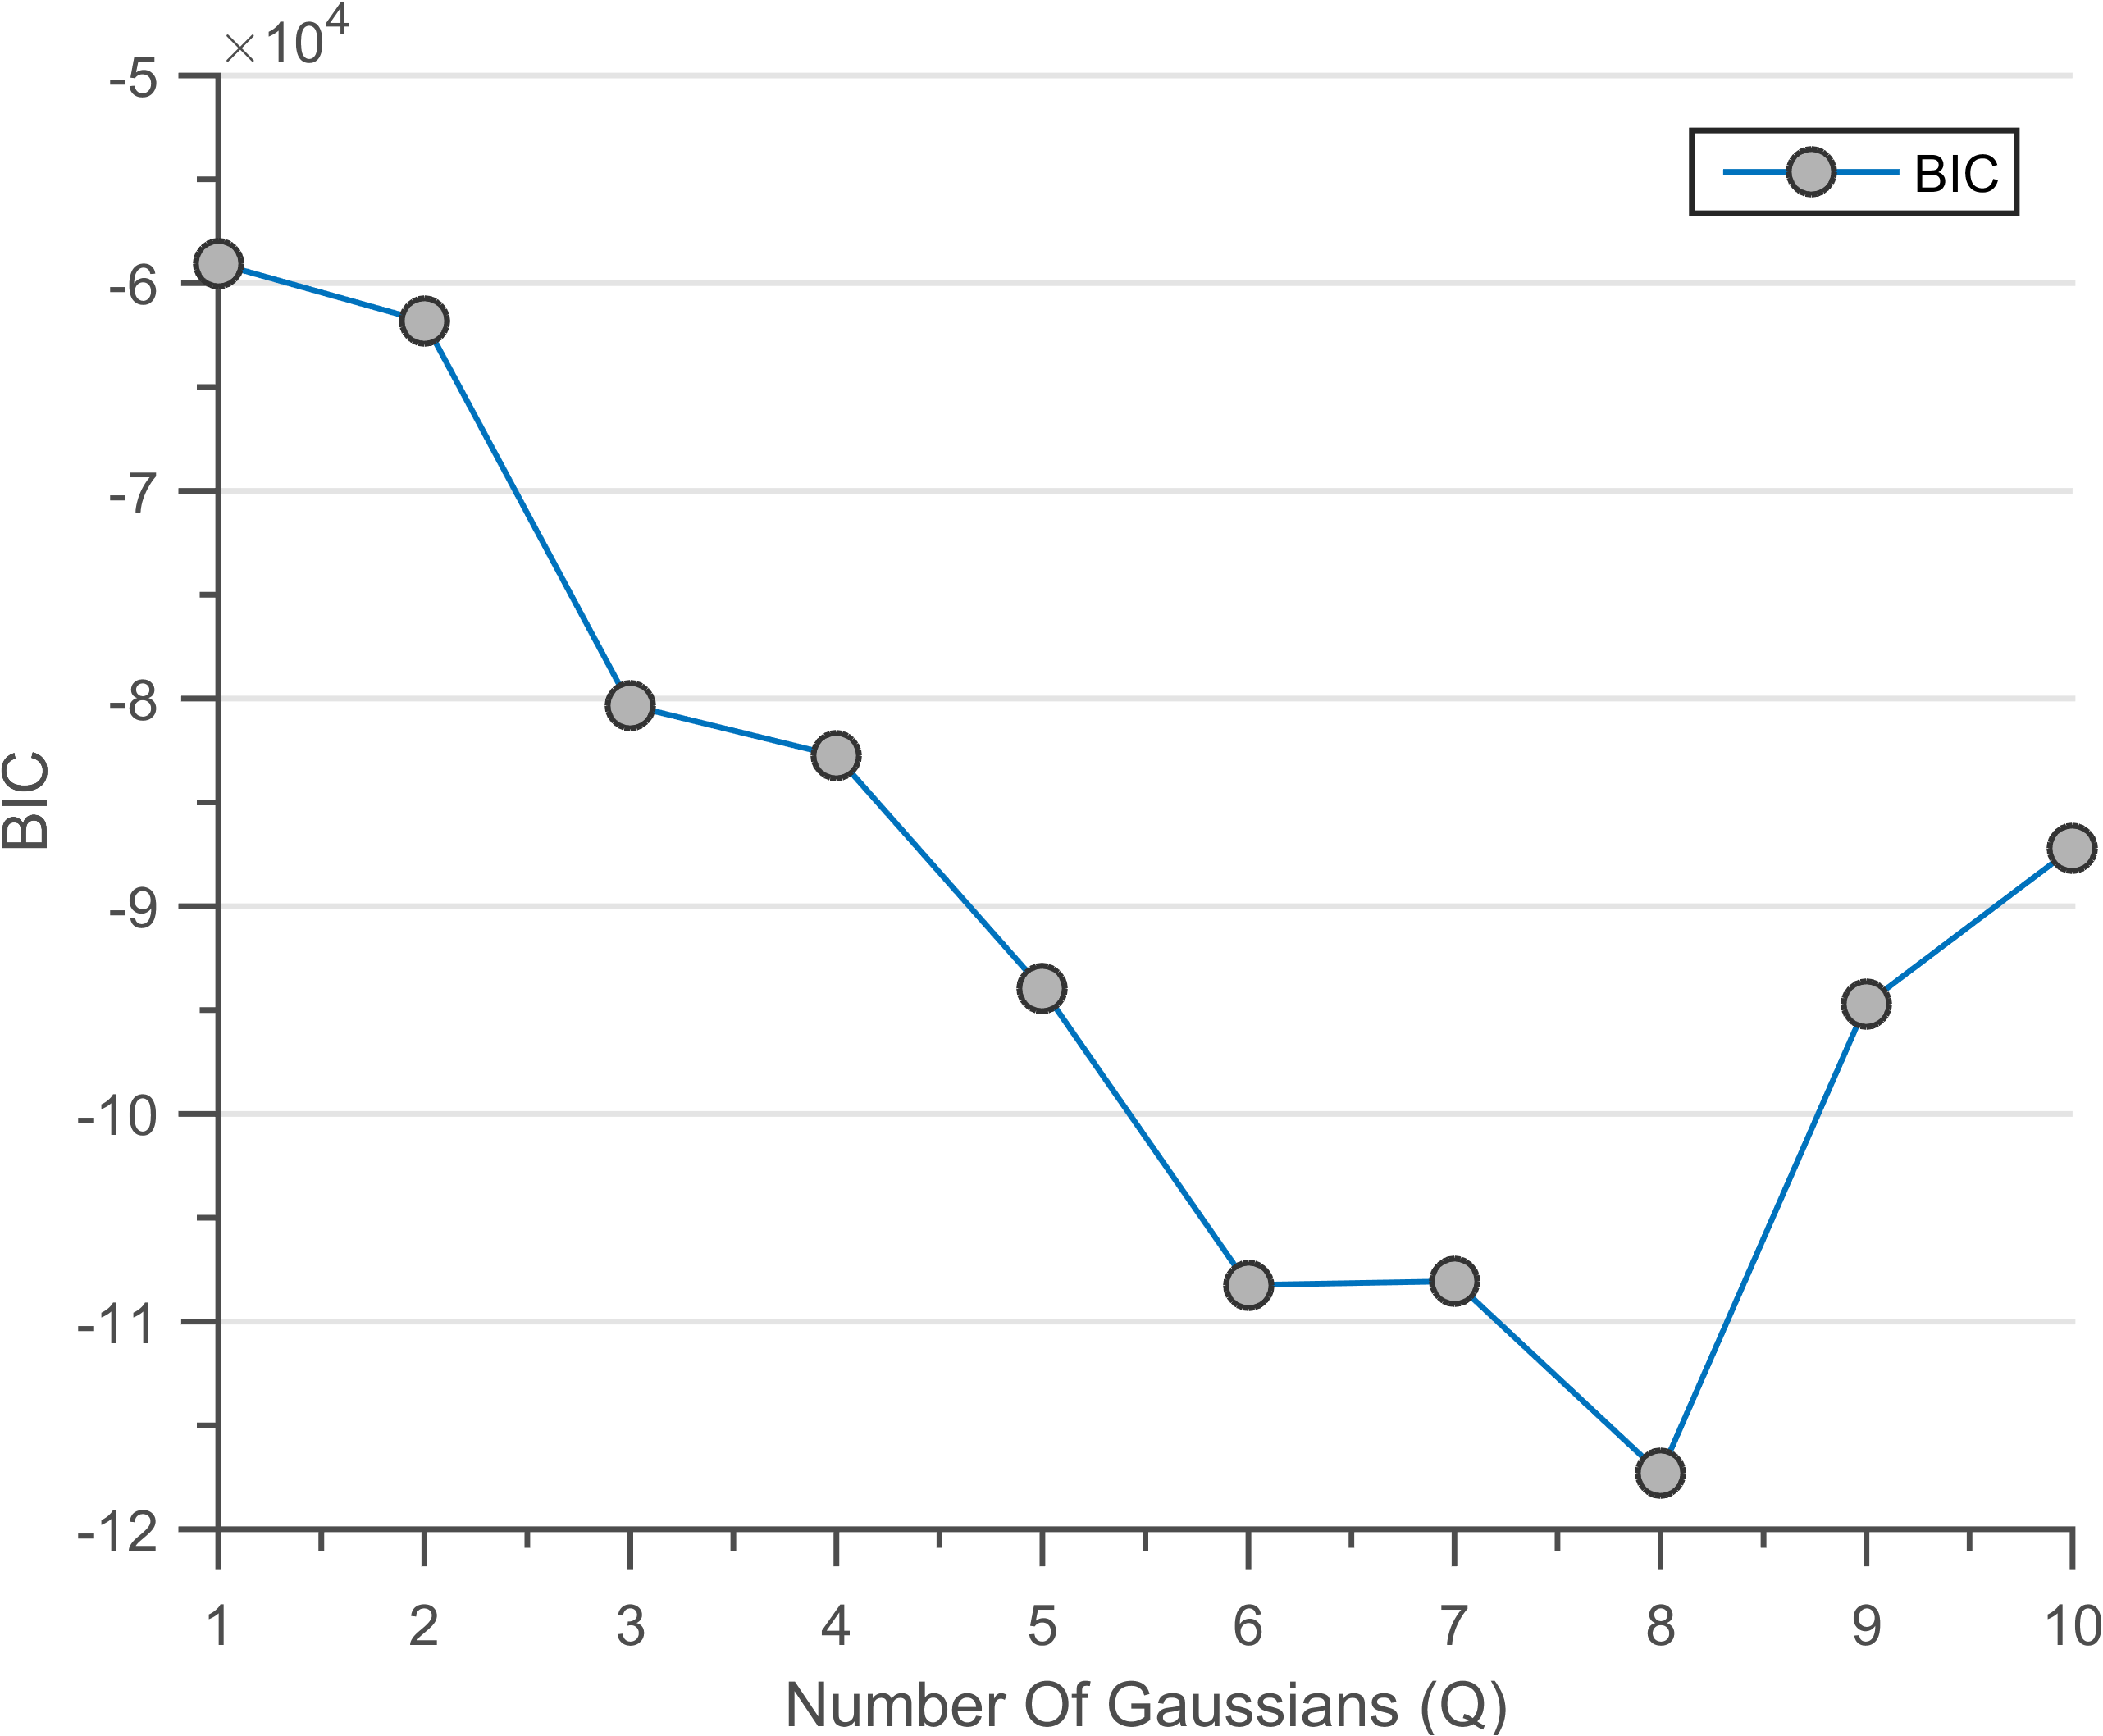
\includegraphics[width=0.45\textwidth]{imagesPart2/bicVsQ_HTCBuilding}\label{subfigBICHTC}}\quad
  
  \caption{Results of spectral mixture kernels on real data from HTC building}
\end{figure*}

Figure \ref{subfigStablizationHTCData} shows the stabilization diagram with increasing number of gaussians $Q$. We can observe that as the number of $Q$ increases the algorithm starts finding better and better modes. We can observe that there are three modes which start stabilizing from $Q=5$. The, figure \ref{subfigBICHTC} shows the BIC criterion with increasing number of Gaussian's $Q$. We can see that that the BIC is minimum for $Q=8$ and hence if we add anymore Gaussians for our dataset we will be performing over-fitting. 

In the current setting of the Spectral Mixture model we propose an automatic way to identify the most important frequencies of a structural system. Neither the mode shapes nor the damping ratios are estimated in the current format. In future we would like to derive a method to estimate mode-shape and damping ratio such that the contributions of neighbouring Gaussians are also taken into account. Without doubt this is very nascent stage of application of Spectral Mixture Kernel for system identification and there remains problems such as identification of mode-shape and damping ratio in this algorithm. We wish to tackle these problems in the future. 

\section{Non-stationary kernels}\label{nonStationaryKernels}
The Spectral mixture kernel creates a huge variety of stationary covariance functions. But there also exist a great many number of non-stationary covariance functions which can have interesting properties. 

\subsection{Linear Kernel} \label{subSecCh4LinearKernel}
The Bayesian Linear regression described during section \ref{secBayesianModelling} can also be seen as a form of GP Regression but with a Linear covariance function. In the Bayesian linear regression we assume a prior distribution of parameters, this is equivalent to assuming a prior distribution over functions. For a function and its prior as defined by equation \ref{eqBLRRevisited}.

\begin{equation}\label{eqBLRRevisited}
    f(x_{i}) = \phi(x_{i})^{T}w
\quad \quad \Pr[w] = \mathcal{N}(0, \Sigma_{Prior}) 
\end{equation}

The equivalent prior over the functions \(f\) can be written as equation \ref{eqPriorDistributionOverLinearFunctions}

\begin{equation}\label{eqPriorDistributionOverLinearFunctions}
    \Pr[f(x)] = GP(0, \phi(x)^{T} \Sigma_{Prior} \phi(x'))
\end{equation}

The above covariance function (\(k(x, x') = \phi(x)^{T} \Sigma_{Prior} \phi(x')^{T}\)) describes a family of functions which are linear combinations of the basis functions (\(\phi(x)\)). Hence a linear basis describes family of linear functions, while a polynomial basis encodes a family of polynomial basis functions. If we assume an independent noise \(\epsilon\) on the observations then based on the discussion on noisy GPs (section \ref{subSecPosteriorNoisy}) the GP prior becomes:

\begin{equation}\label{eqNoisyPriorDistributionOverLinearFunctions}
    \Pr[y(x)] = GP(0, \phi(x)^{T} \Sigma_{Prior} \phi(x') + \sigma_{n}^2\delta_{xx'})
\end{equation}

The matrix \(\Sigma_{Prior}\) and \(\sigma_{n}\) are the hyper-parameters of this GP prior and \(\phi(x)\) represents its functional form. The hyper-parameters can be chosen using marginal likelihood and posterior prediction can be performed based on the discussion on section \ref{secHyperParameter}. 

\paragraph{Revisiting Bayesian Linear Regression}\label{paraLinearGPExperiment}
Let us revisit the experiment performed in section \ref{secBayesianModelling} but this time using GP regression and a linear kernel. The toy-dataset \(\mathcal{D}_{1} = \{X = [-0.5, 0.33, 0.66], Y = [0, 0.5, 0.5]\}\) (section \ref{secBayesianModelling}) will be used again. The prior distribution on parameters \(\Sigma_{Prior} = [w_{0}, 0; 0, w_{1}] \mid w_{0} = 1, w_{1} = 1\) and prior on noise \(\sigma_{n} = 0.1\) will be the same as used in the earlier experiment. \(w_{0}\), \(w_{1}\) and \(\sigma_{n}\) are the hyper-parameters of this GP prior. 

Figure \ref{subFigdrawsLinear} shows draws from a GP prior with mean zero and Linear kernel as defined in the above paragraph. The solid black line defines the mean function, shaded blue region defines 95\% confidence interval (2\(\sigma\)) distance away from the mean. The dashed lines are five functions drawn at random from a GP prior. Random functions drawn from a linear GP are linear. Figure \ref{subFigposteriorLinearNoisy_1} show draws from a GP posterior with mean zero and Linear kernel  as defined in above para and conditioned on the first data point \(X = -0.5, Y = 0\). The solid black line defines the mean function, shaded blue region defines 95\% confidence interval (2\(\sigma\)) distance away from the mean. The dashed lines are five functions drawn at random from a GP prior. The posterior mean passes from the data point, random functions drawn from a linear GP are linear.


\begin{figure}[!ht]
  \centering
    \subfigure[{Draws from a GP prior with mean zero and Linear kernel (\(k(x, x') = \phi(x)^{T} \Sigma_{Prior} \phi(x')^{T} + \sigma_{n}^2\delta_{xx'}\)) with \(w_{0} = 1, w_{1} = 1\) and \(\sigma_{n} = 0.1\). The solid black line defines the mean function, shaded blue region defines 95\% confidence interval (2\(\sigma\)) distance away from the mean. The dashed lines are five functions drawn at random from a GP prior. Random functions drawn from a linear GP are linear.}]
  {
        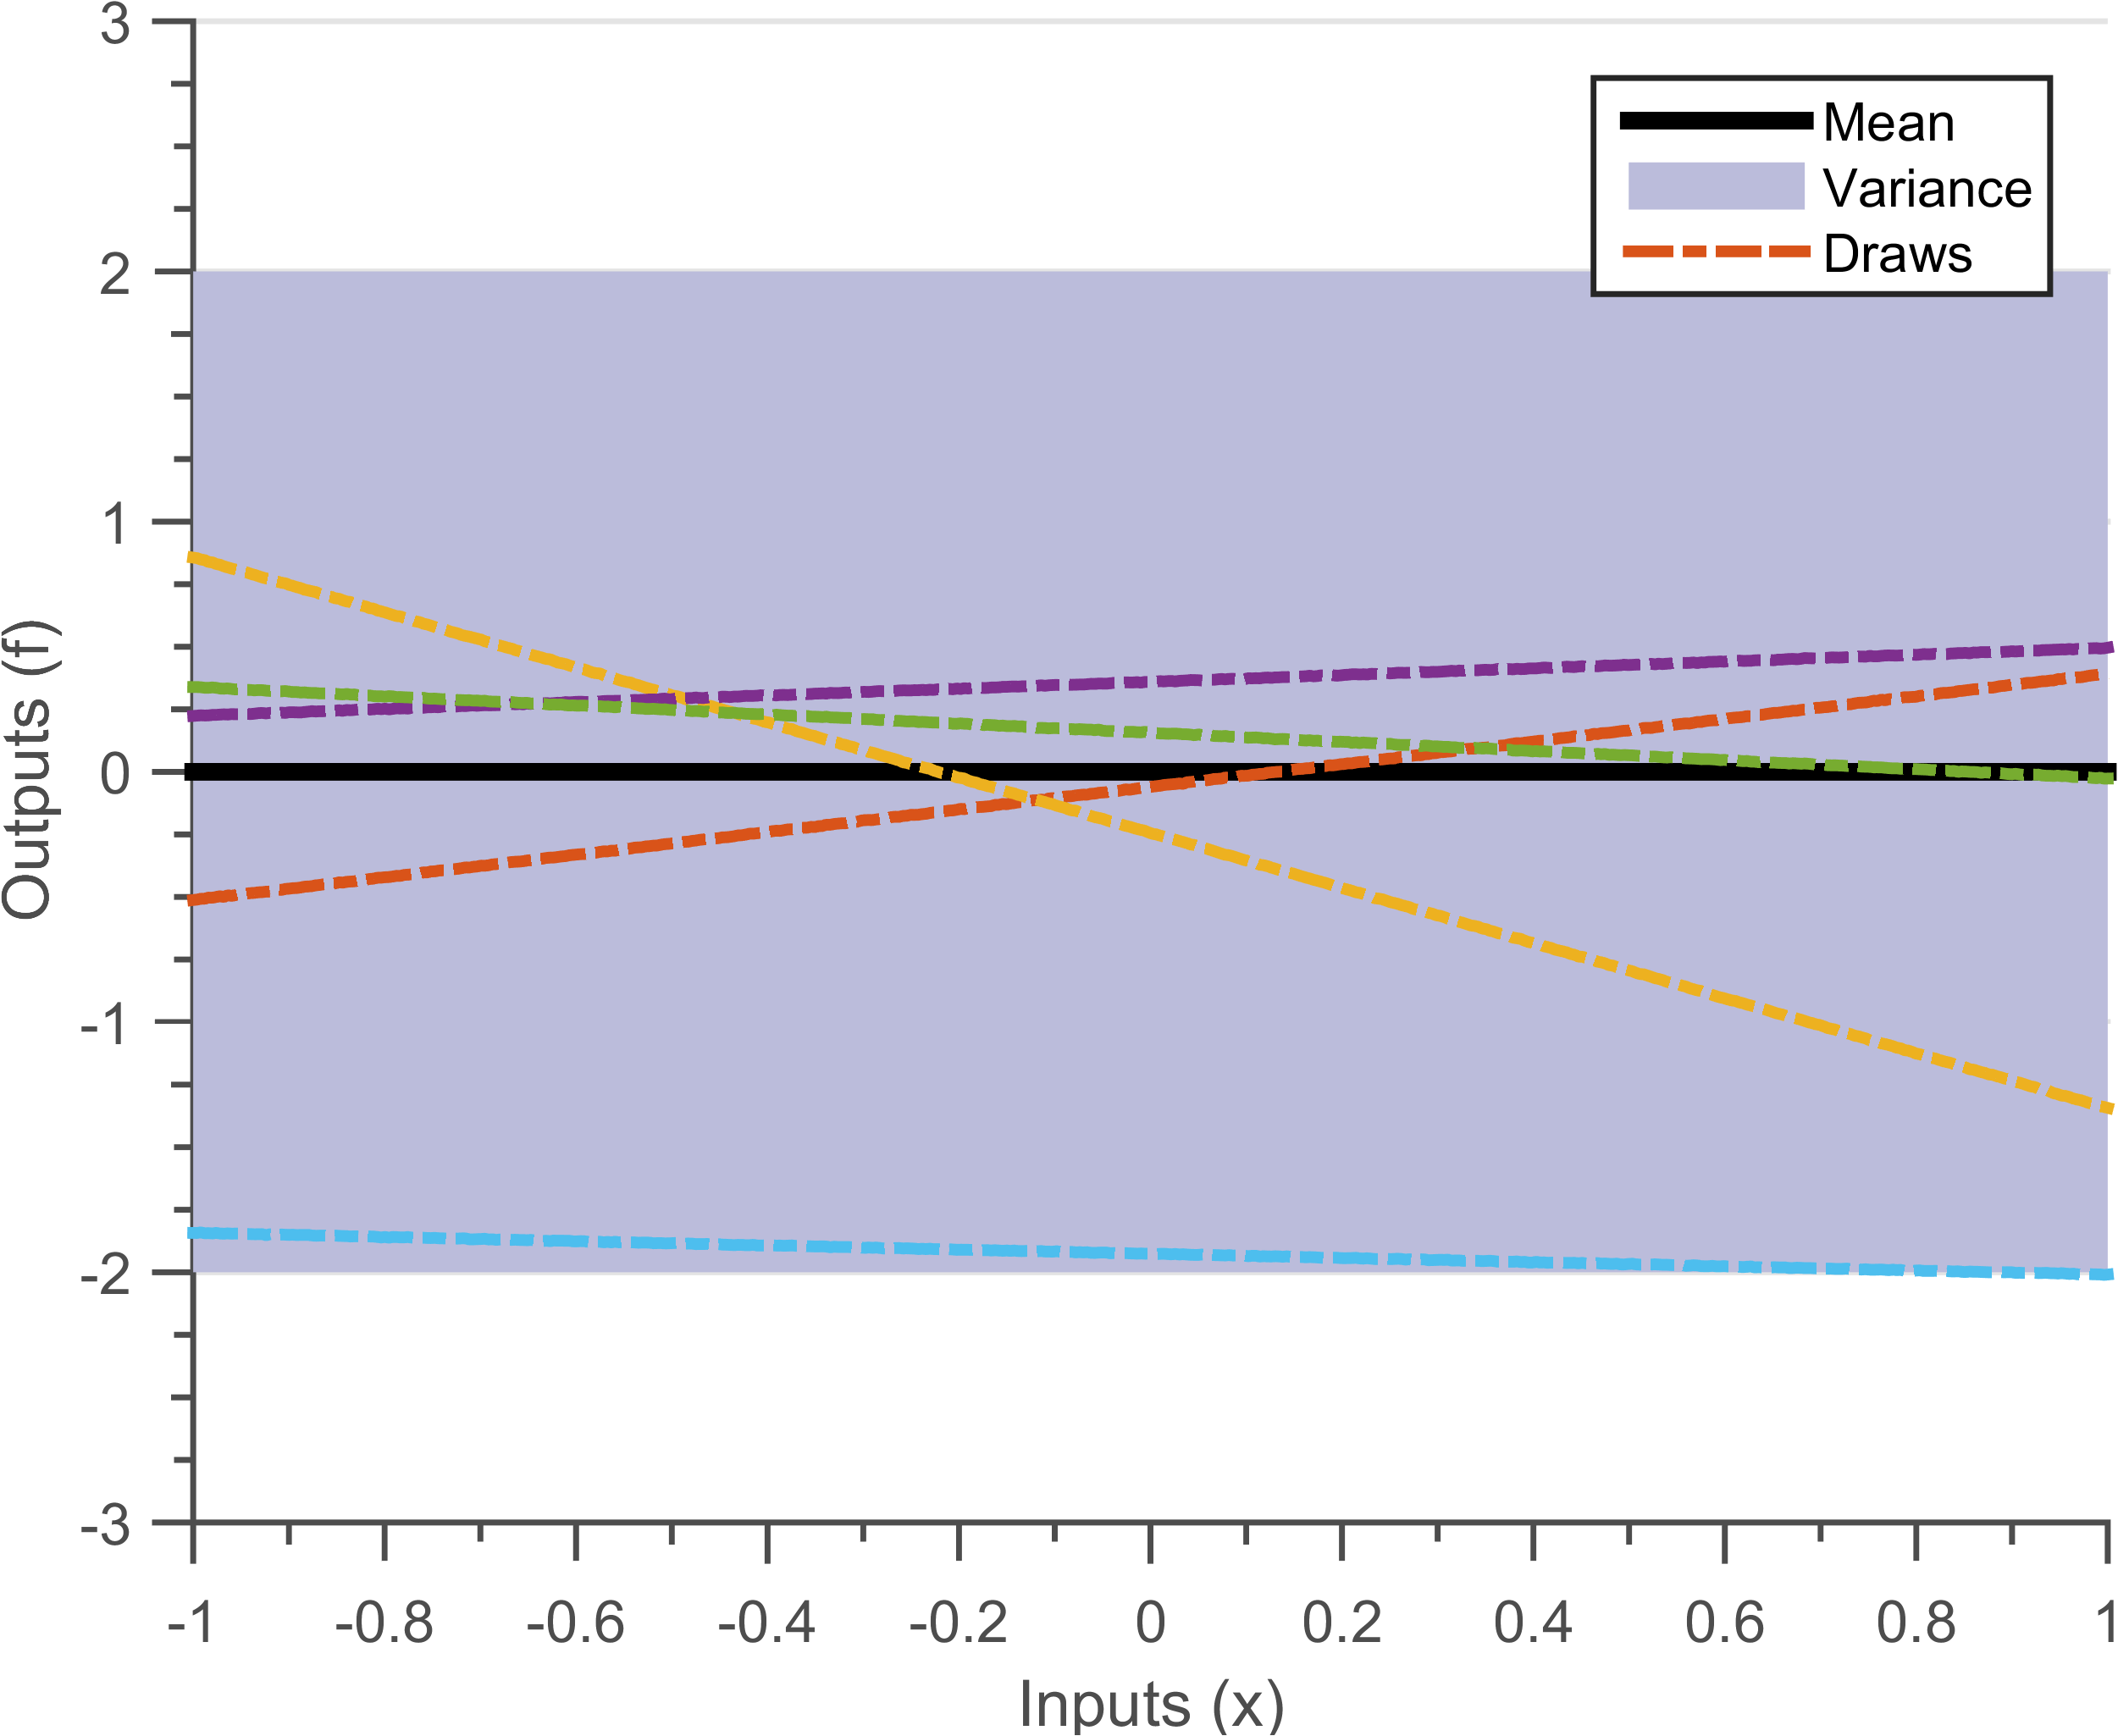
\includegraphics[width=0.45\textwidth]
        {imagesPart2/drawsLinear}
        \label{subFigdrawsLinear}
  }\quad
\subfigure[{Draws from a GP posterior with mean zero and Linear kernel (figure \ref{subFigdrawsLinear}) conditioned on the data \(X = -0.5, Y = 0\). The solid black line defines the mean function, shaded blue region defines 95\% confidence interval (2\(\sigma\)) distance away from the mean. The dashed lines are five functions drawn at random from a GP prior. The posterior mean passes from the data point, random functions drawn from a linear GP are linear}]
  {
        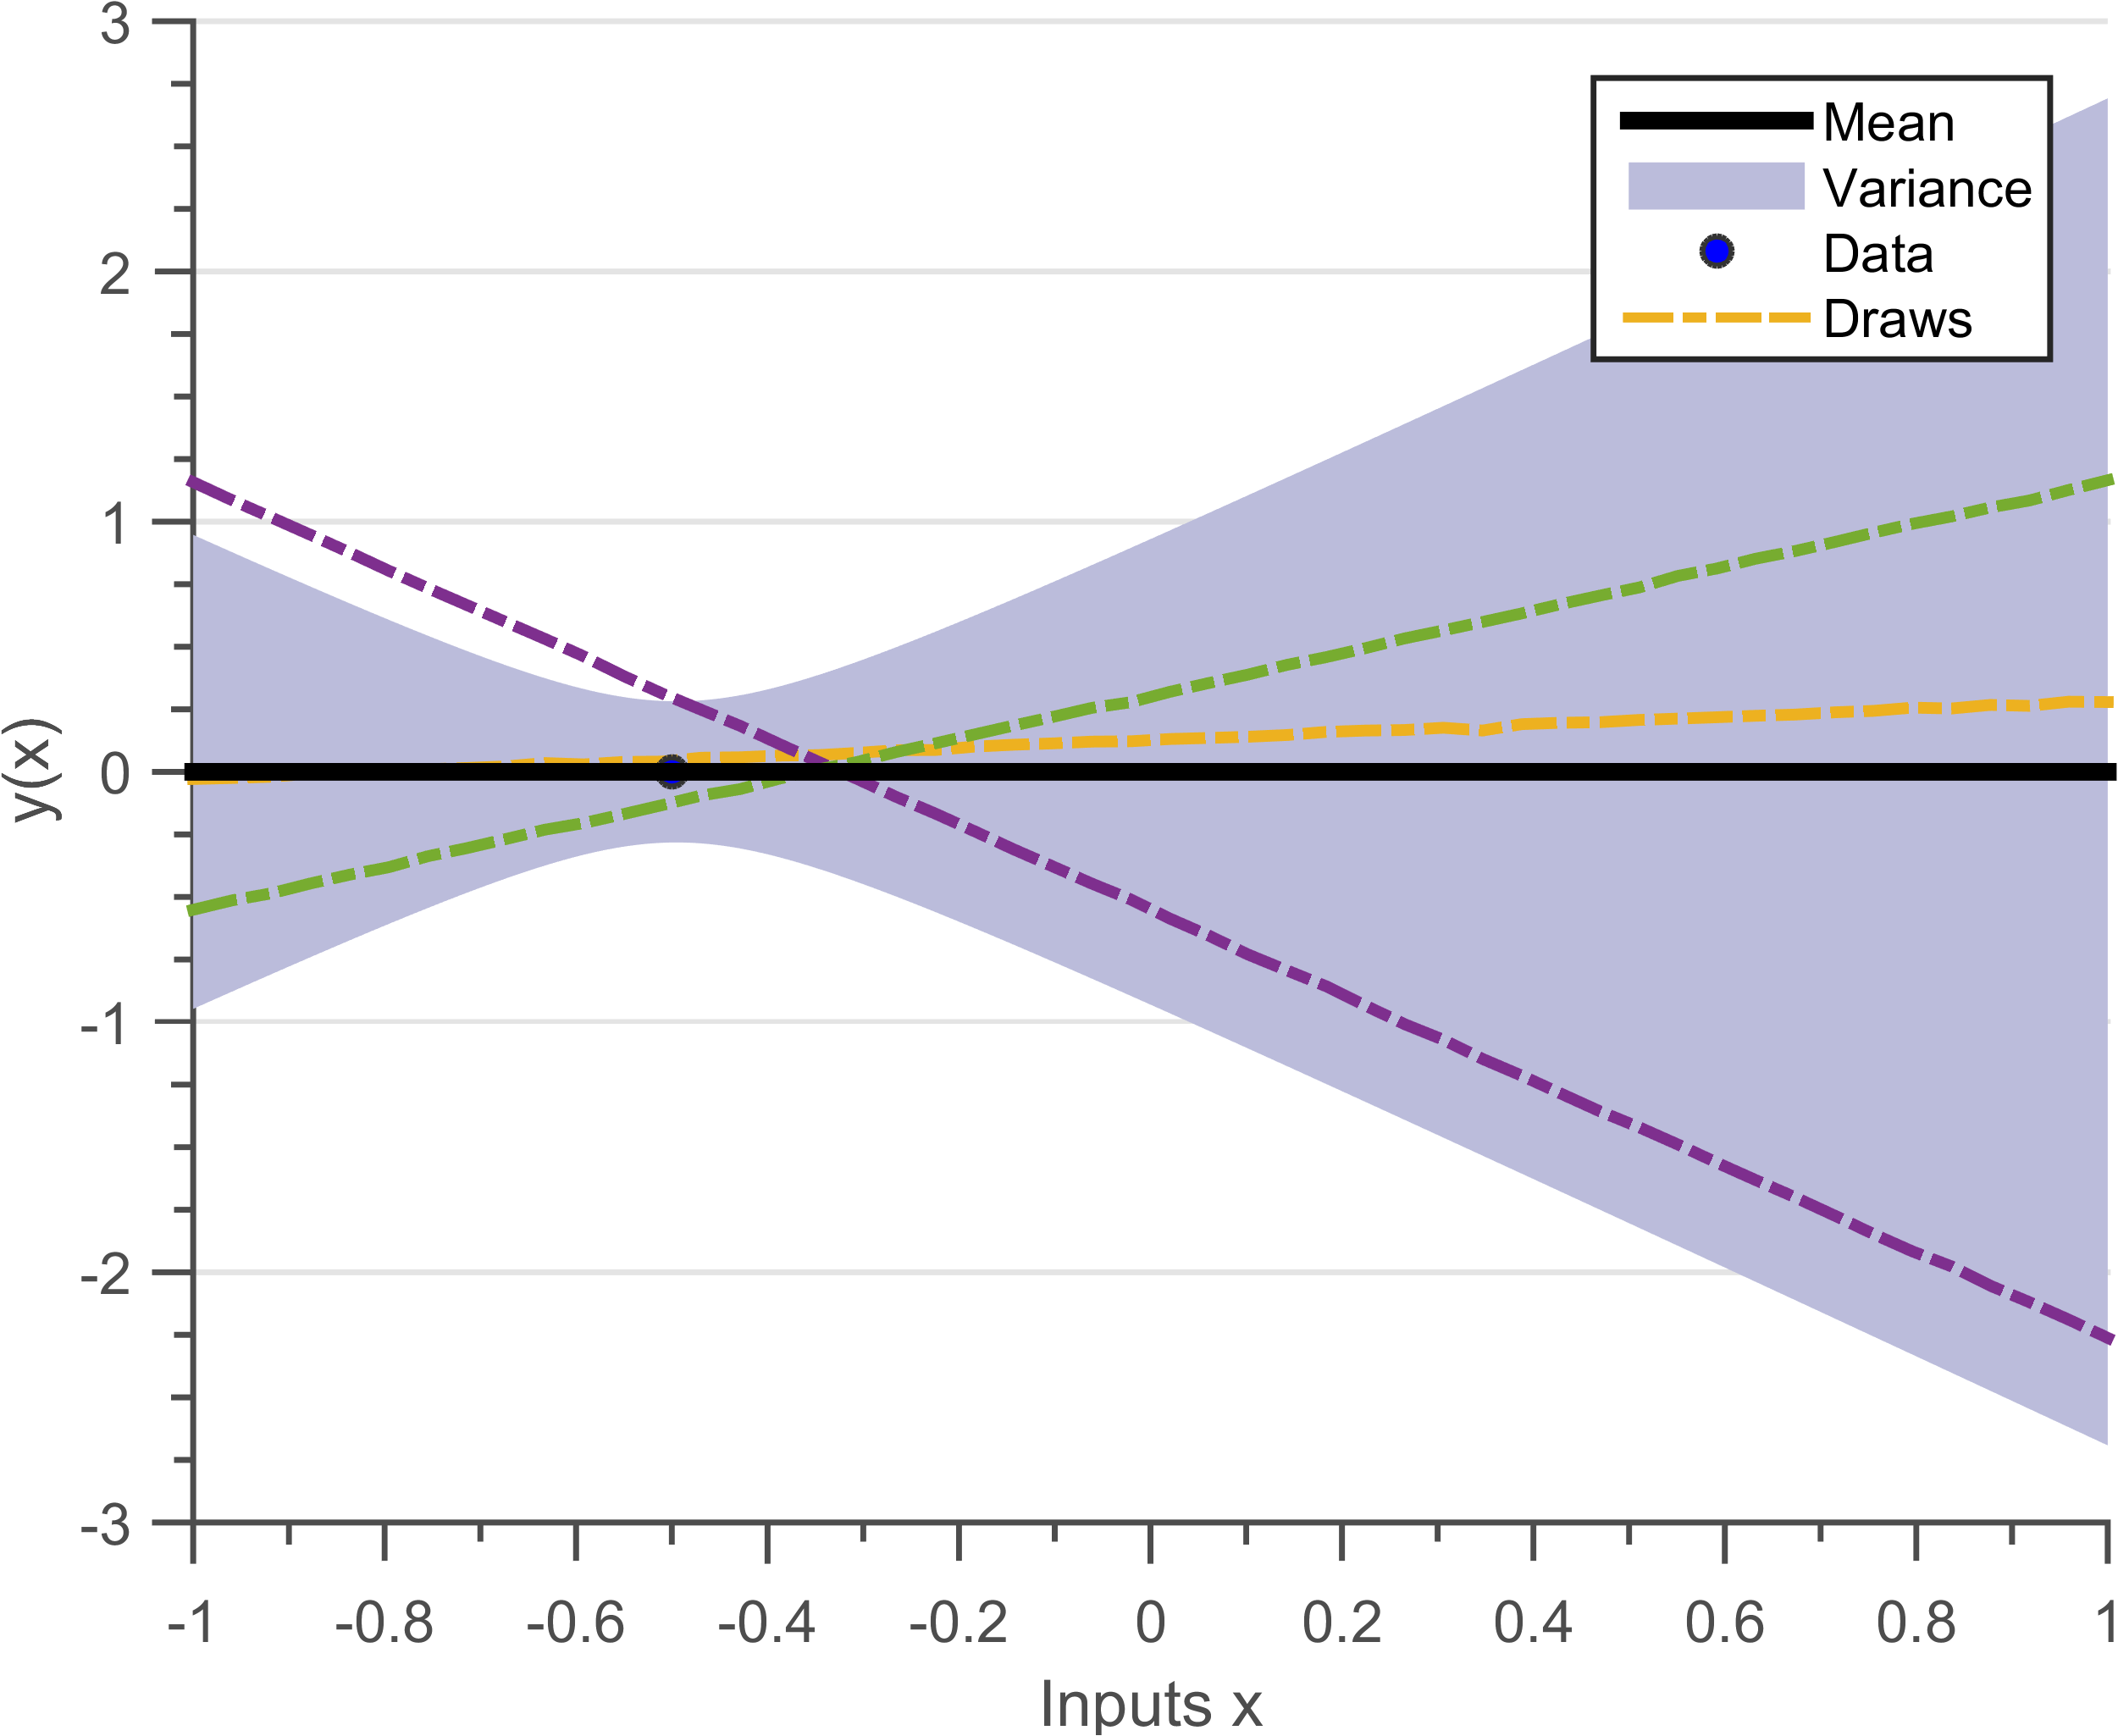
\includegraphics[width=0.45\textwidth]
        {imagesPart2/posteriorLinearNoisy_1}
        \label{subFigposteriorLinearNoisy_1}
  }\quad

       \caption{Prior and posterior from a GP prior of linear kernel}
       \label{figPriorAndPosteriorLinearKernel}
\end{figure}

Figure \ref{subFigmaximizingMarginalLikelihoodLinear} shows the contours of marginal likelihood with respect to \(w\). The marginal likelihood is maximum for \(w_{0} = 0.2576, w_{1} = 0.4584\), incidentally the same as posterior predictions in section \ref{toyDataSet1}. This means that the data has the highest possibility of coming from a dataset defined by such a prior. Figure \ref{subFigoptimizedPosteriorLinearNoisy_3} shows the posterior for same data set but for the hyper-parameters where marginal likelihood is maximum.

\begin{figure}[!ht]
  \centering
    \subfigure[{Marginal likelihood contours for varying bias and slope parameter. The noise hyper parameter is \((\sigma_{1} = [0.1])\). Marginal likelihood is maximum for \(w_{0} = 0.2576, w_{1} = 0.4584\).}]
  {
        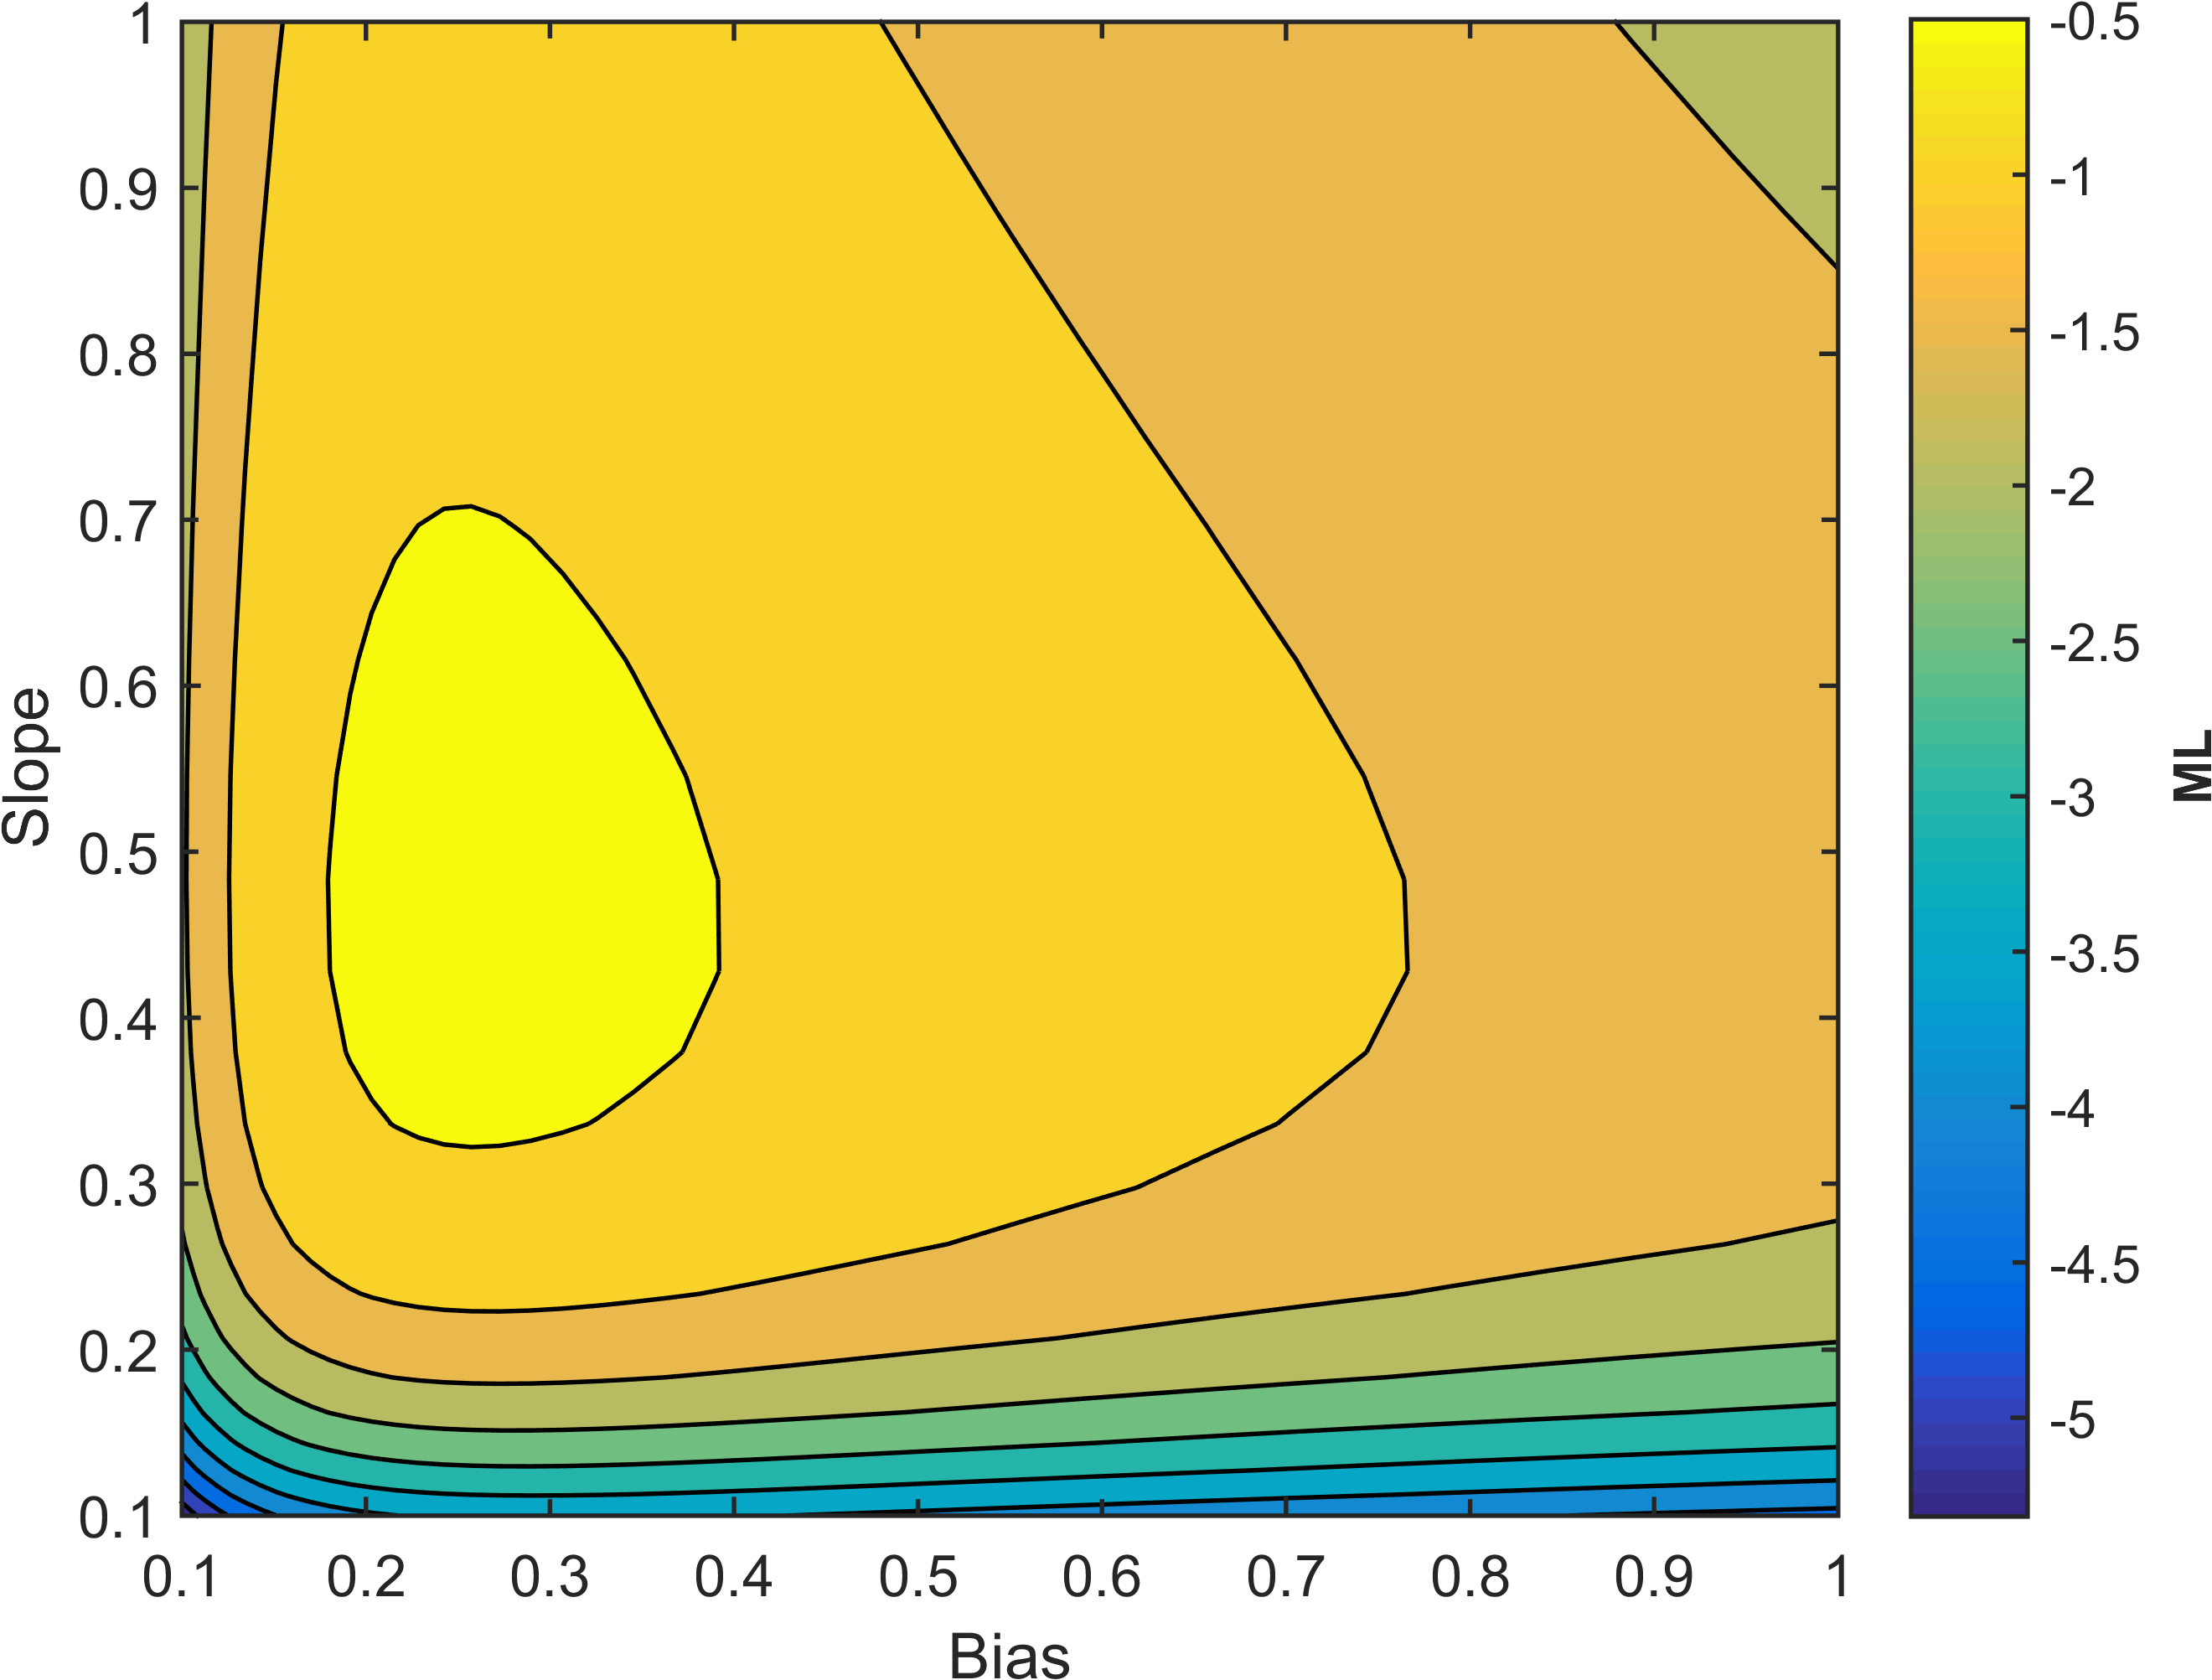
\includegraphics[width=0.45\textwidth]
        {imagesPart2/maximizingMarginalLikelihoodLinear}
        \label{subFigmaximizingMarginalLikelihoodLinear}
  }\quad
\subfigure[{Draws from a GP posterior, conditioned on the dataset \(\mathcal{D}_{1}\) with mean zero and Linear kernel with hyper-parameters that maximize the marginal likelihood.}]
  {
        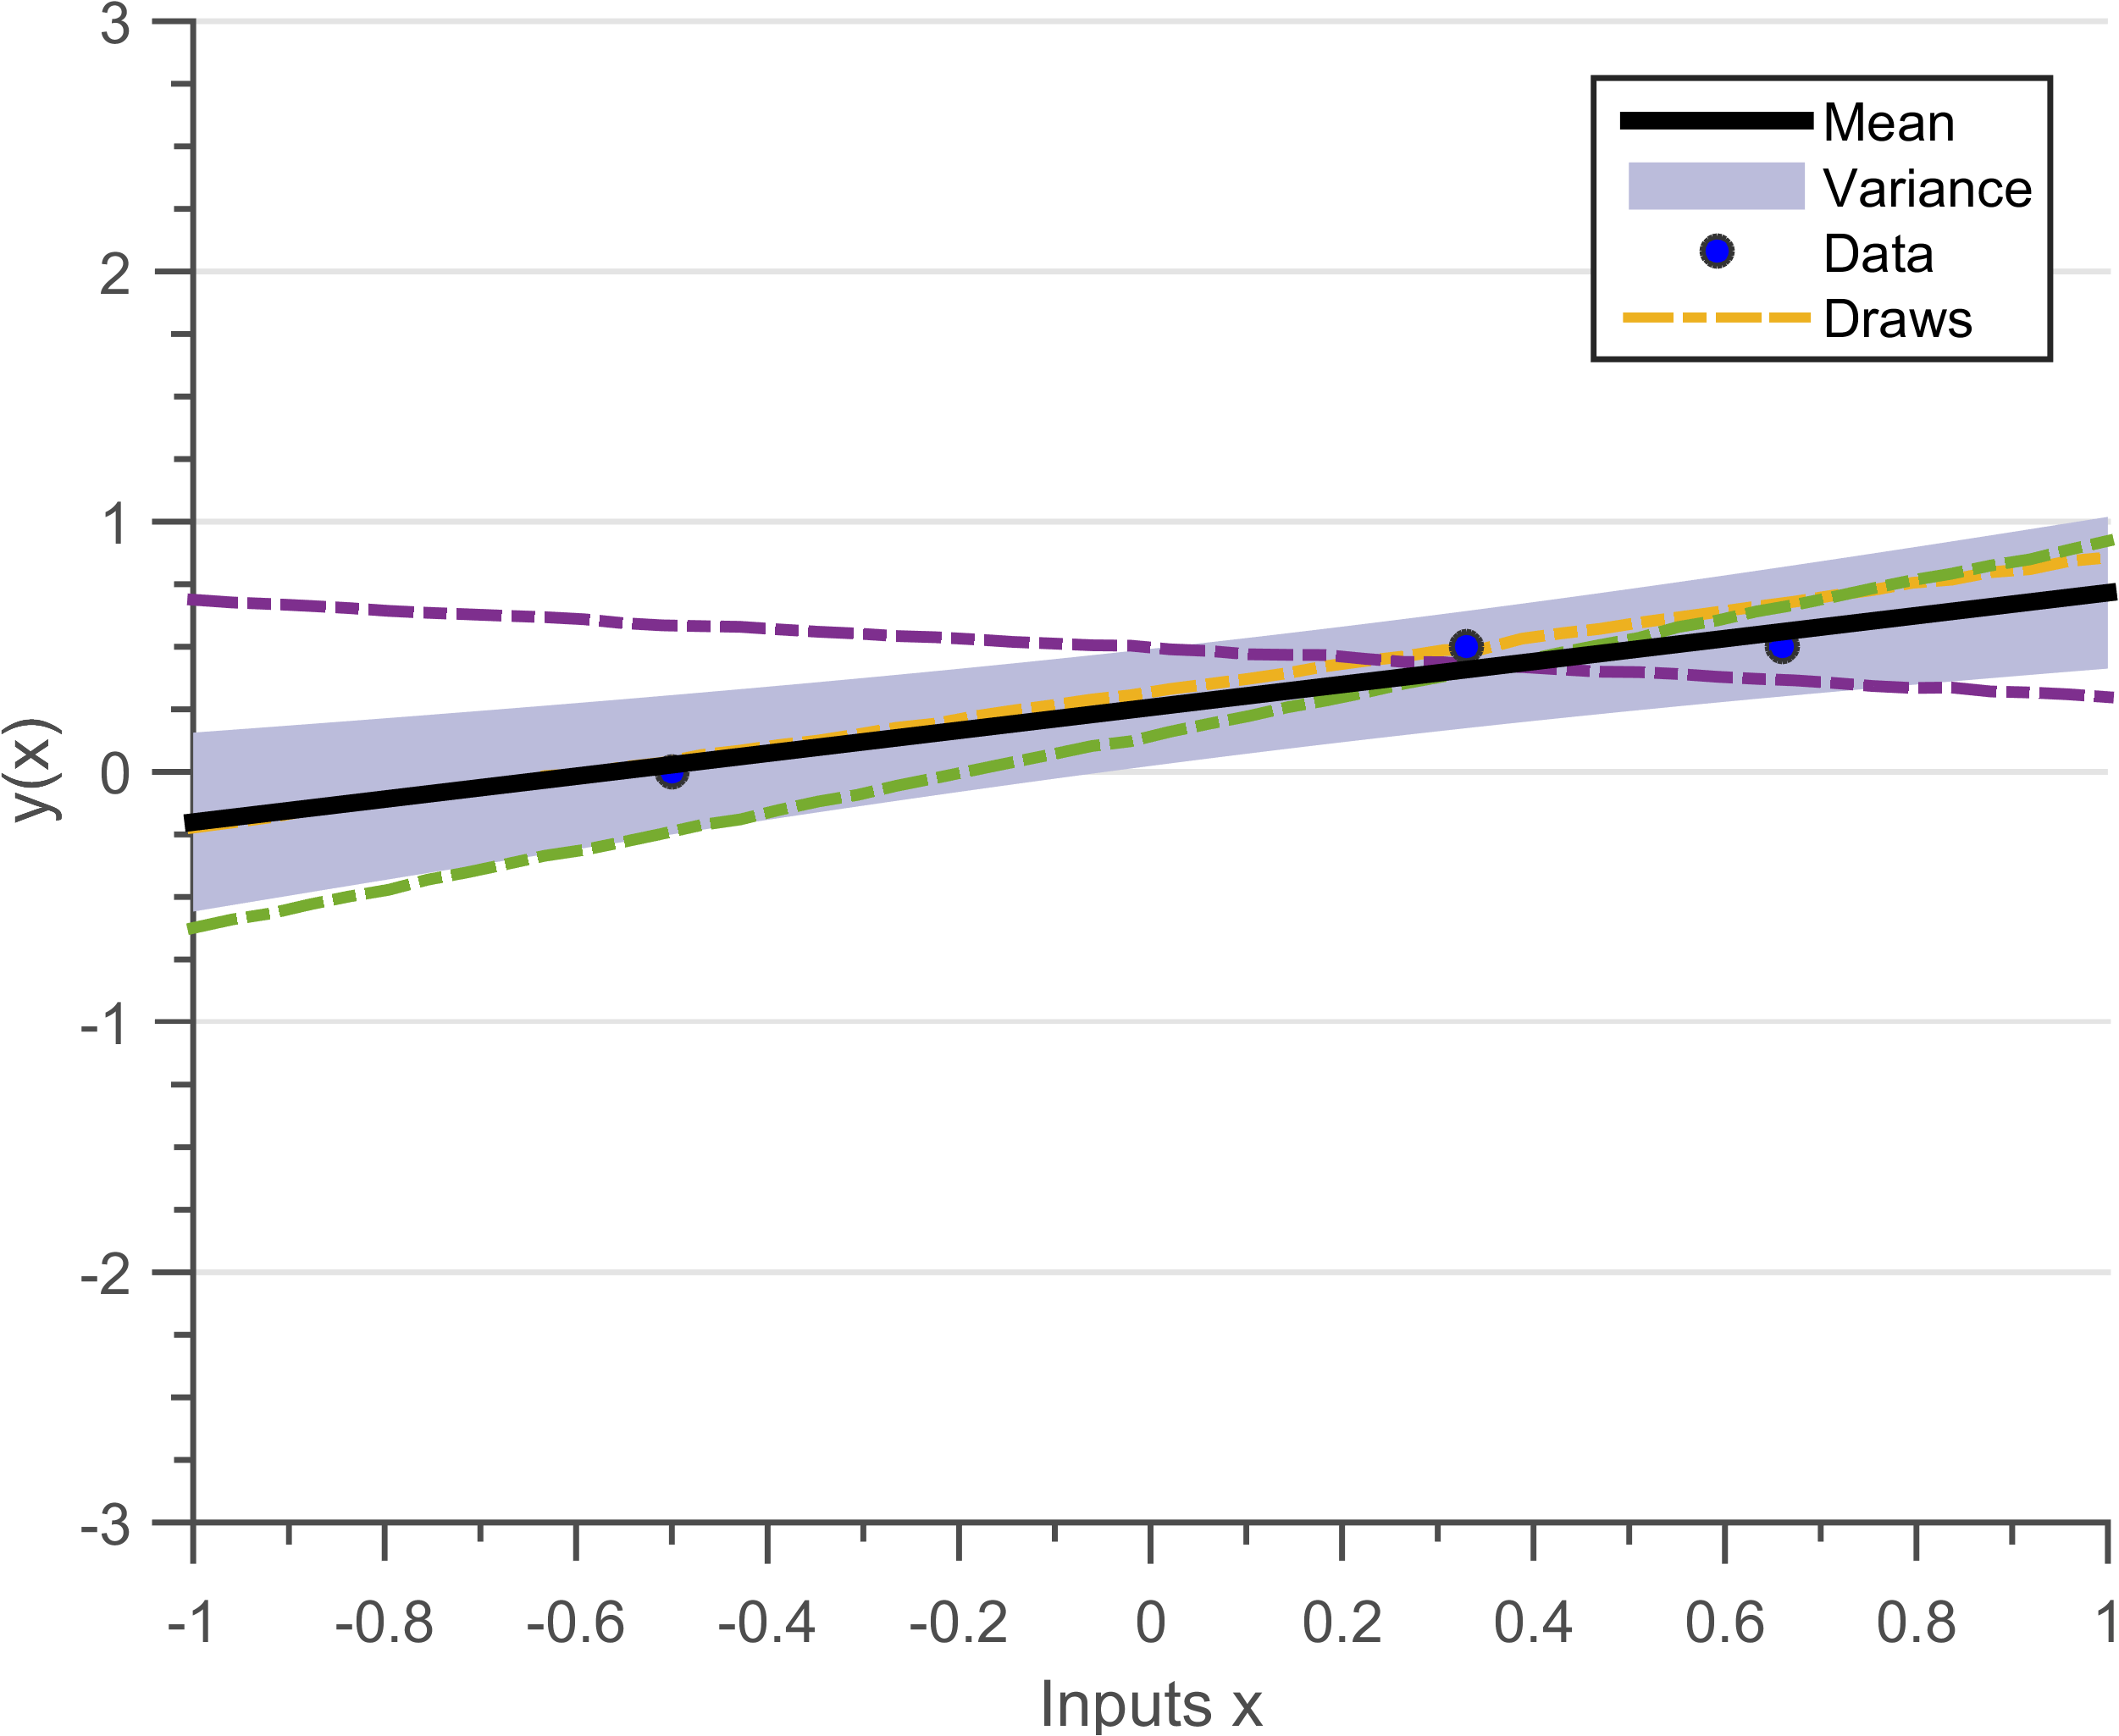
\includegraphics[width=0.45\textwidth]
        {imagesPart2/posteriorLinearNoisy_3}
        \label{subFigoptimizedPosteriorLinearNoisy_3}
  }\quad

       \caption{Maximizing Marginal Likelihood Linear kernel}
       \label{figMaximizingMLLinearKernel}
\end{figure}

\subsection{Neural Network Kernel}\label{subSecCh4NNkernel}
It can be shown that a neural network with infinitely many hidden units and an error activation function (\(erf(z)\) tends to a GP with a Neural network kernel \cite{neal2012bayesian, wilson2014covariance} (equation \ref{eqnNNKernel}). 

\begin{equation}\label{eqnNNKernel}
K_{NN}(x, x', \theta) = \theta_{1}^{2}\frac{2}{\pi} sin^{-1}\left ( \frac{2x\theta_{2}x'}{\sqrt{(1+2x^{T}\theta_{2}x)(1+2x'^{T}\theta_{2}x')}} \right )
\end{equation}

The hyperparameters \((\theta = [\theta_{1}, \theta_{2}])\) are; amplitude \(\theta_{1}\) which defines average distance from mean and the length scale \(\theta_{2}\) which define the smoothness of functions. GP with this covariance function defines a space of superimposed sigmoidal functions. We can use this kernel to embed the information of discontinuity in our family of functions. Figure \ref{figNNPrior} shows random draws from a Neural Network kernel but varying value of hyper parameters. Figure \ref{subfig:drawsNN100} has a higher value of \(\theta_{2}\) than figure \ref{subfig:drawsNN10}, which makes the constituent functions have stronger slope.

\begin{figure*}[!ht]
  \centering
  \subfigure[{Draws from a GP prior with mean zero and Neural Network kernel (equation \ref{eqnNNKernel}) with \(\theta = [1, 10]\).}]
  {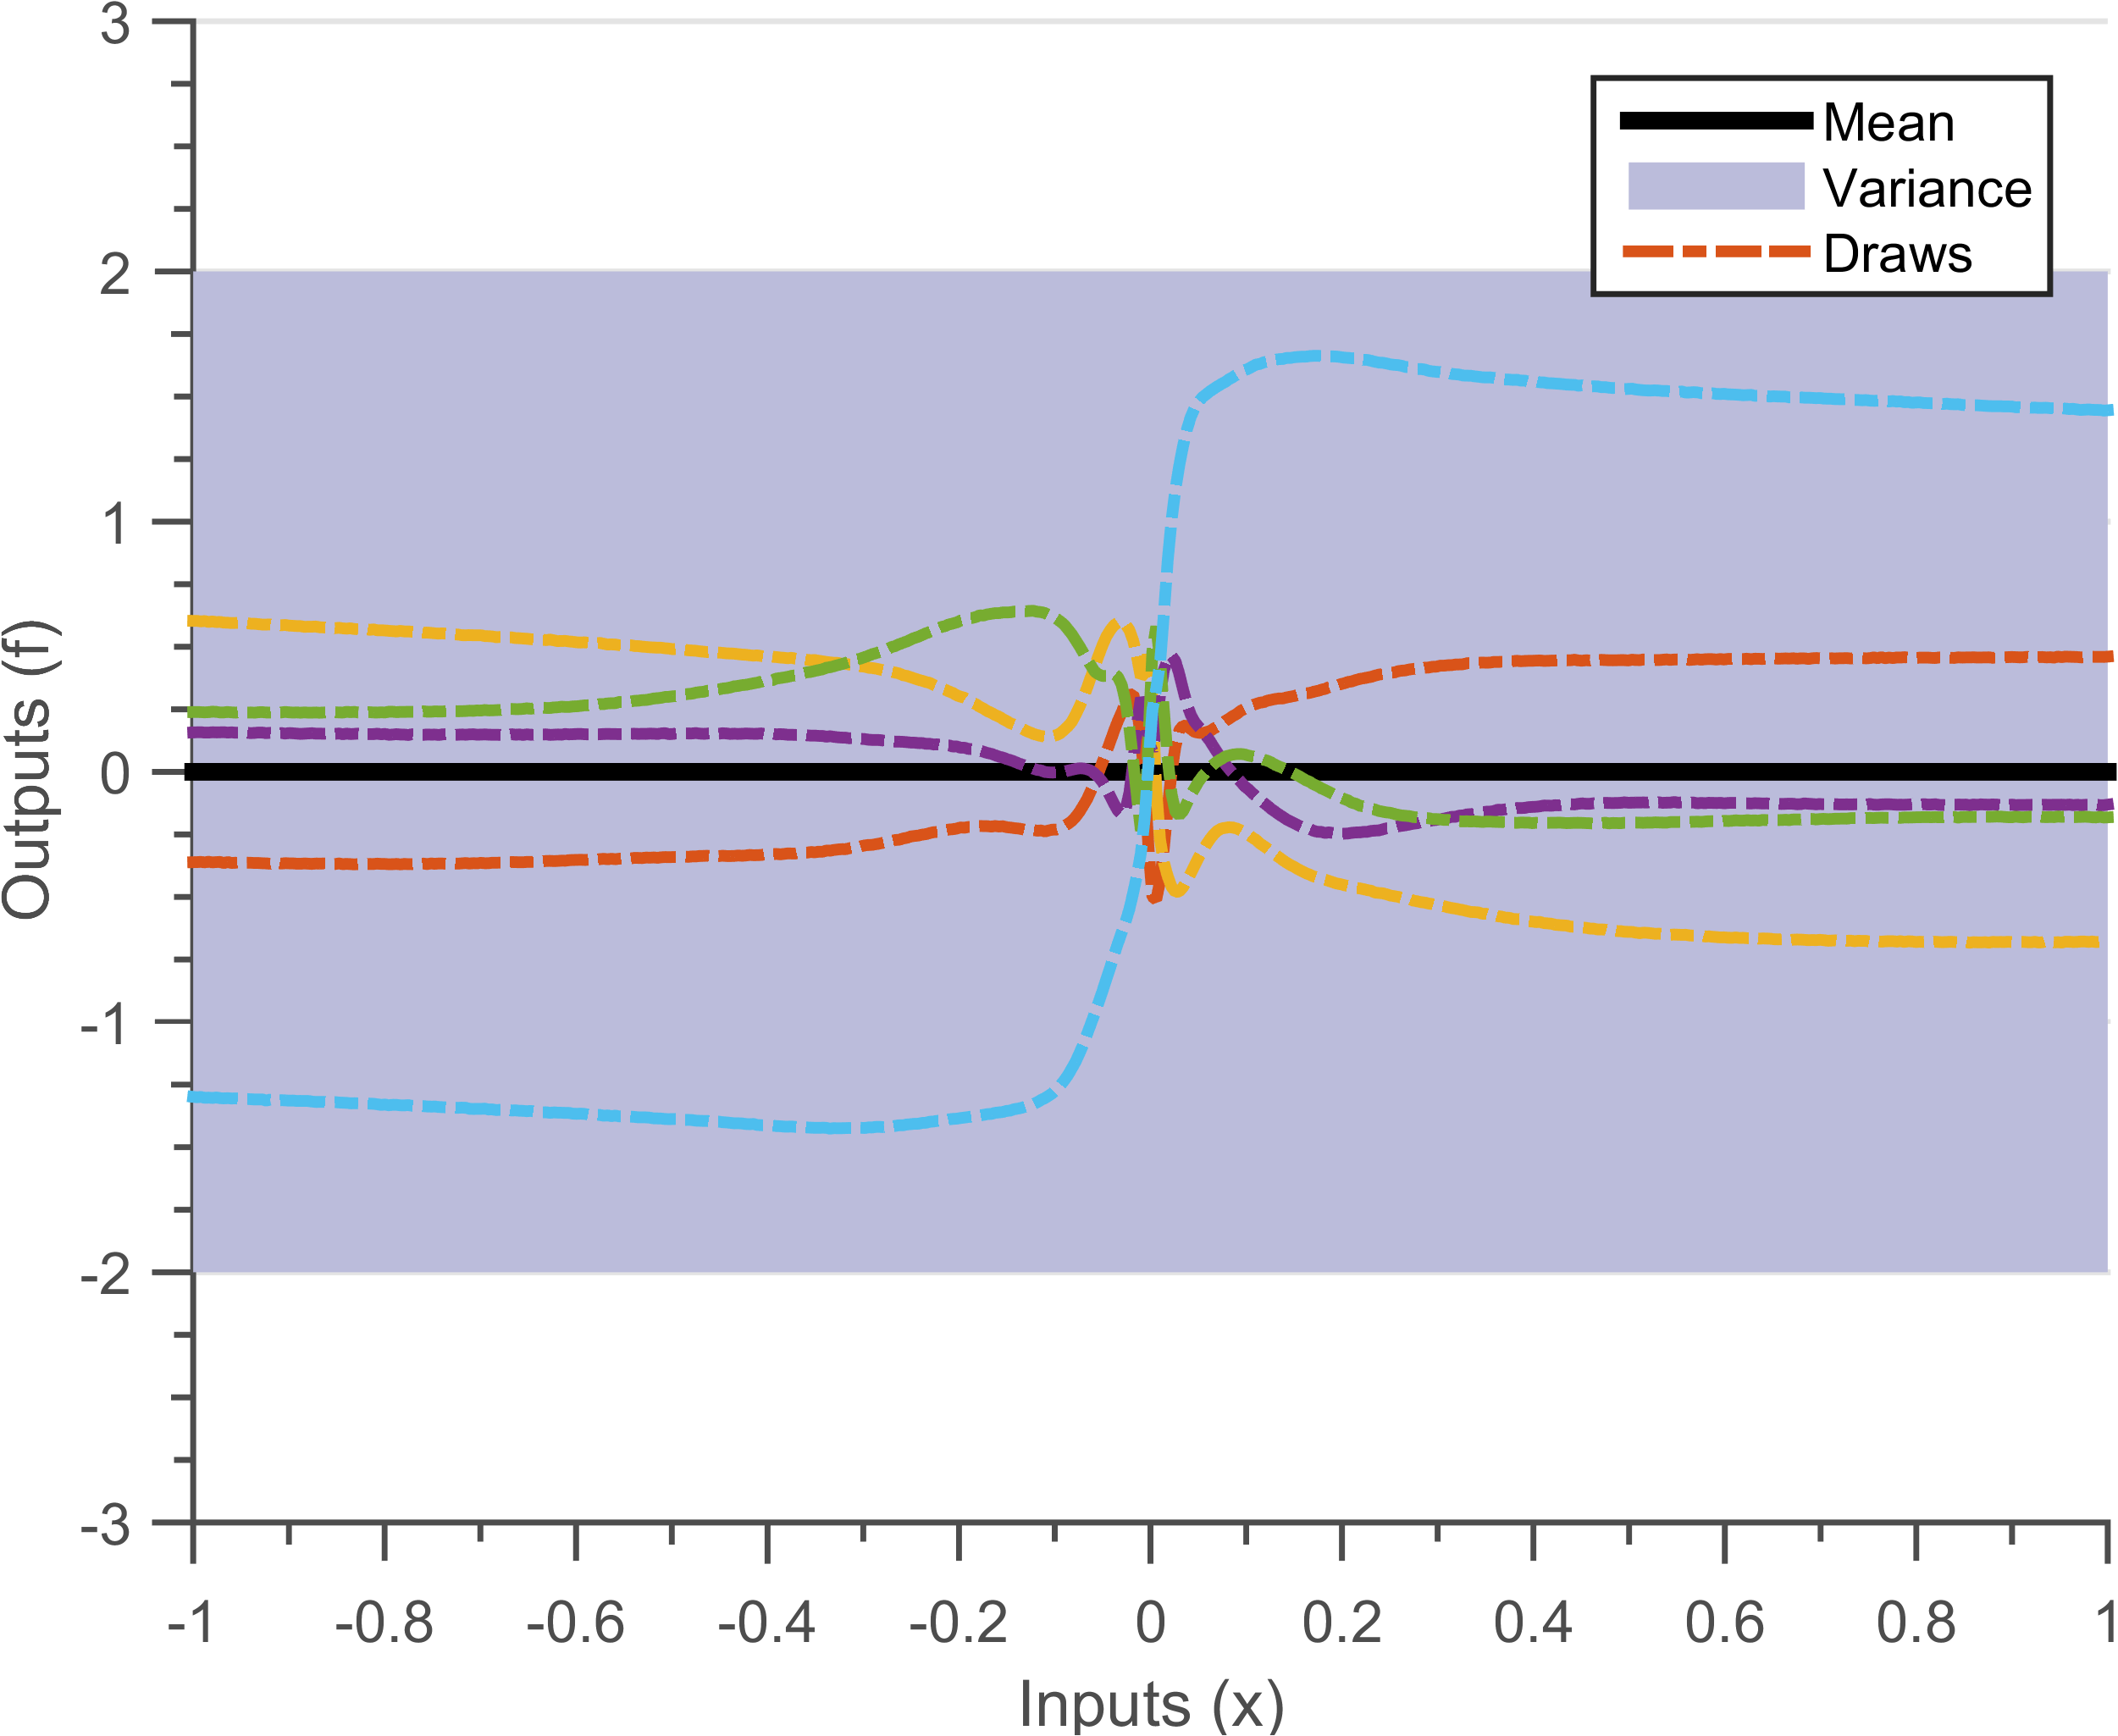
\includegraphics[width=0.45\textwidth]{imagesPart2/drawsNN10}\label{subfig:drawsNN10}}\quad
    \subfigure[{Draws from a GP prior with mean zero and Neural Network kernel (equation \ref{eqnNNKernel}) with \(\theta = [1, 100]\). Higher value of \(\theta_{2}\) signifies increasing slope}]
  {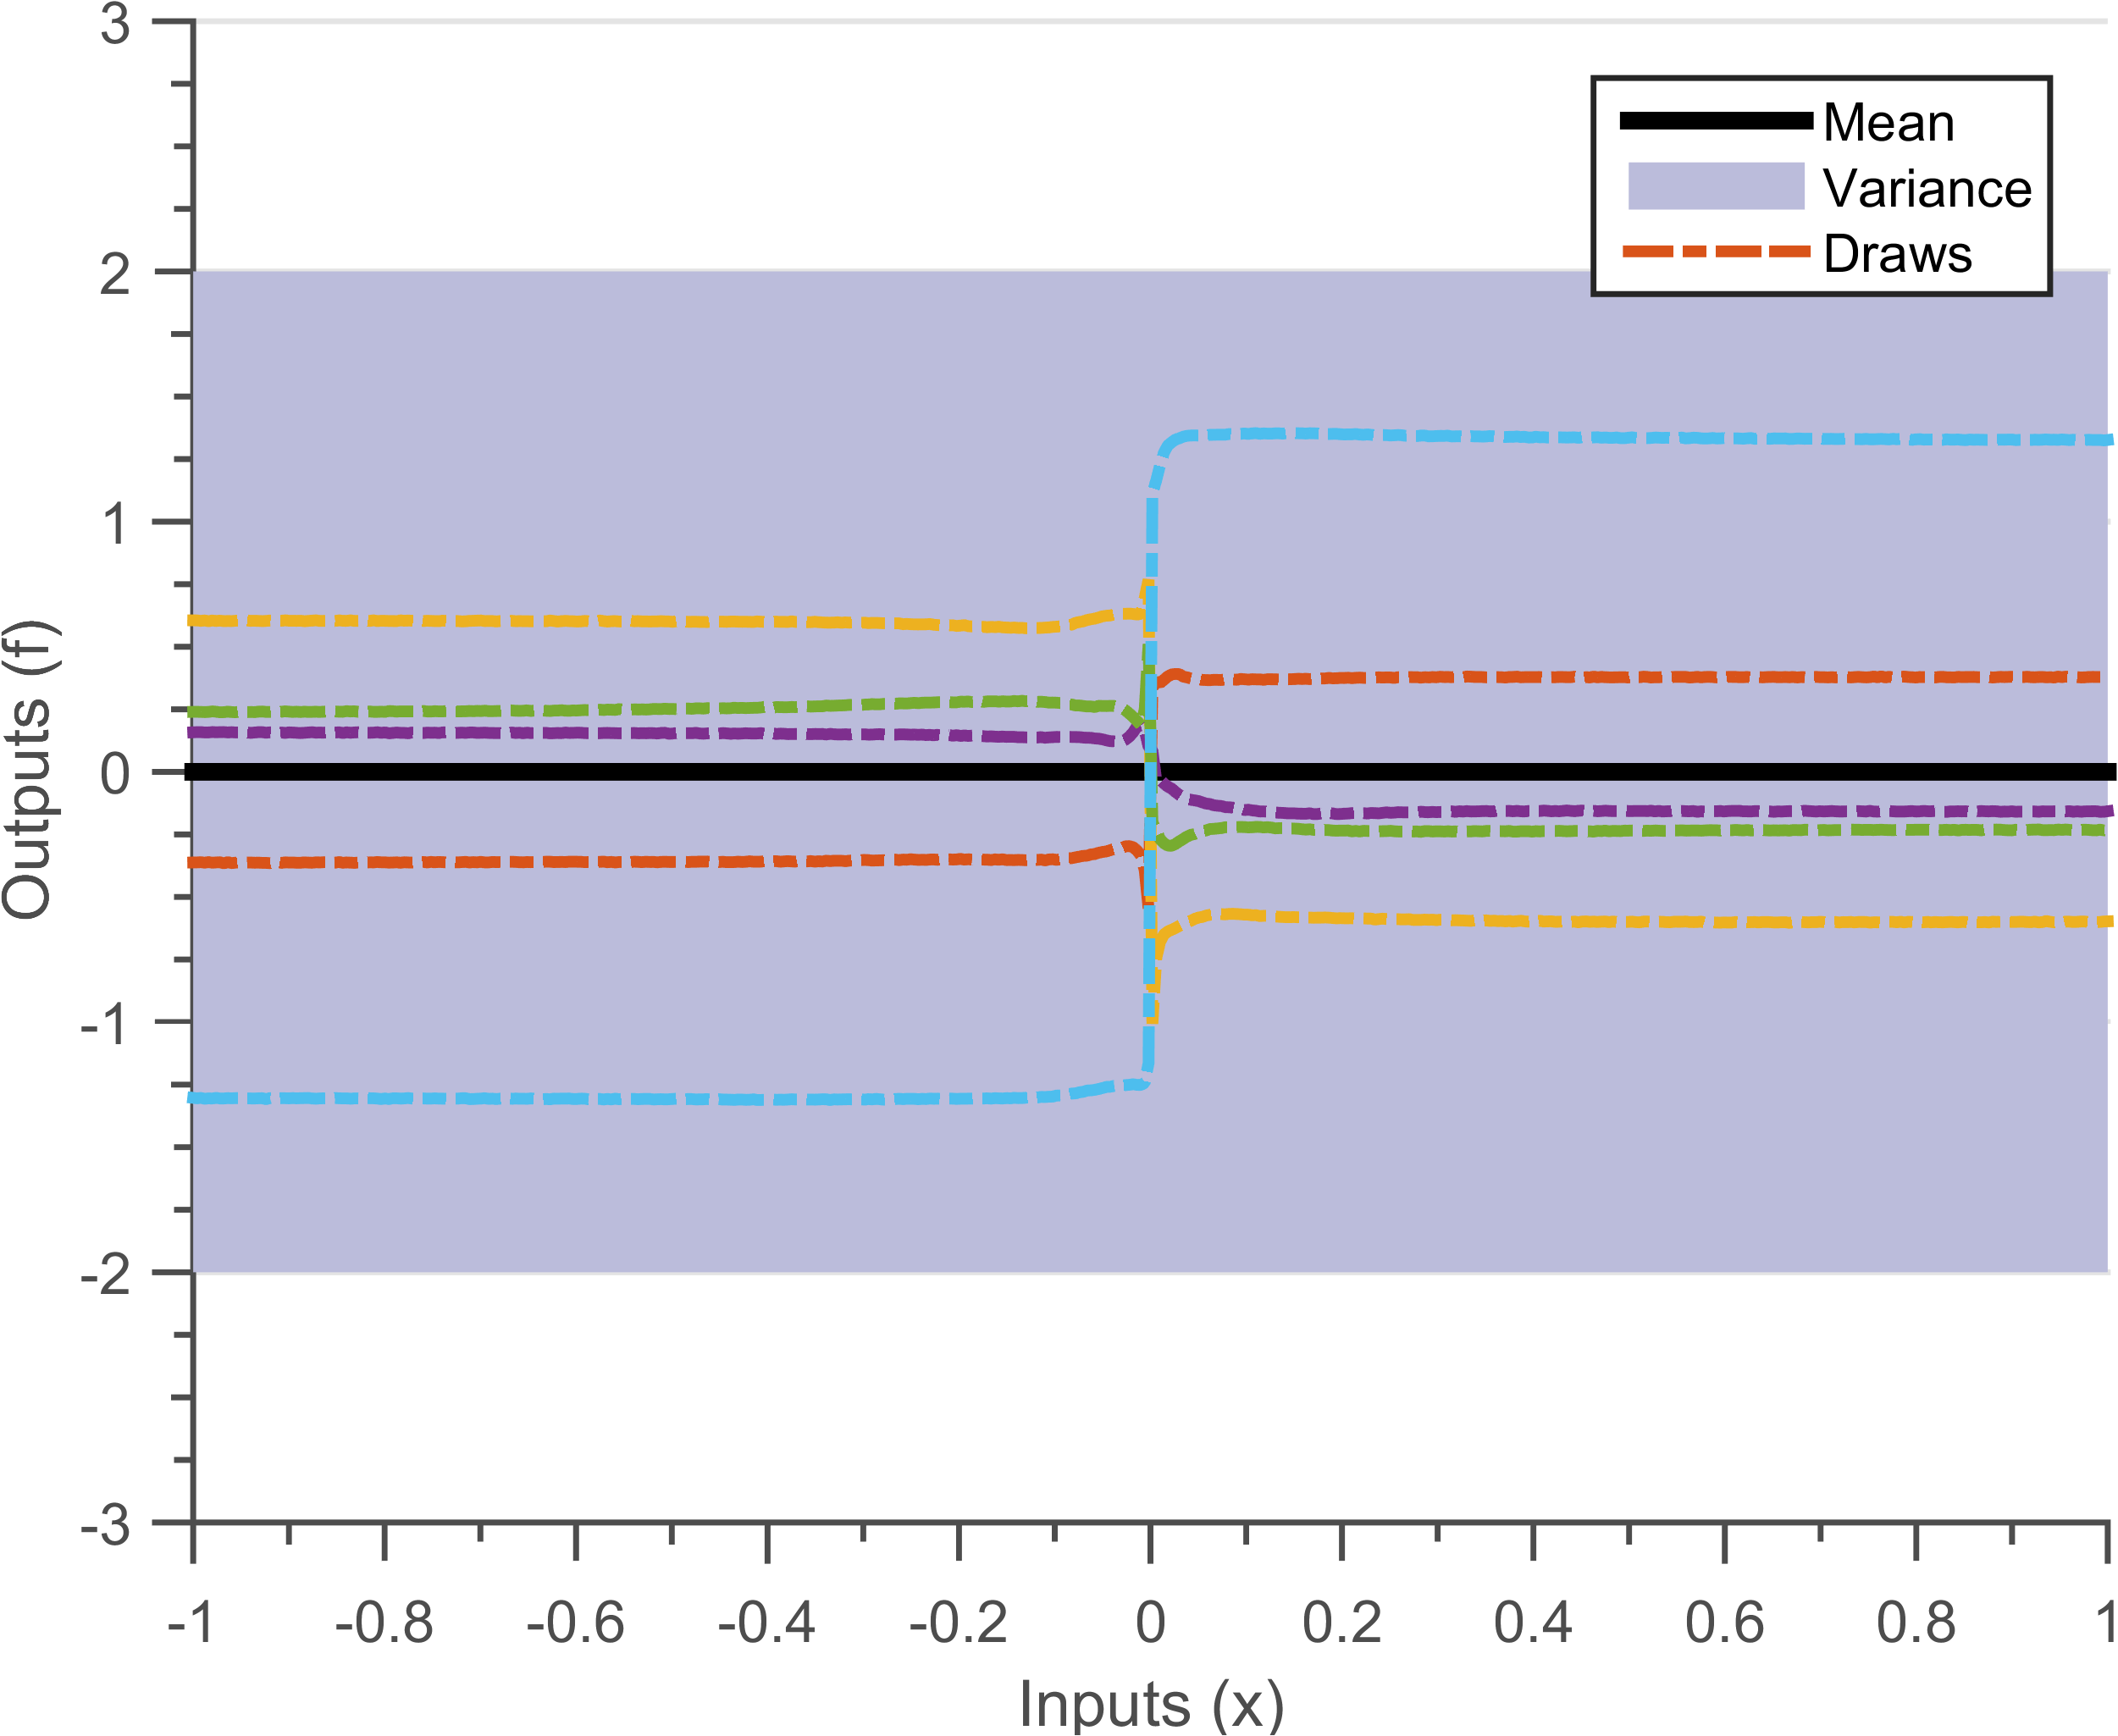
\includegraphics[width=0.45\textwidth]{imagesPart2/drawsNN100}\label{subfig:drawsNN100}}\quad
  \caption{Draws from Neural Network kernels having different hyper-parameters. The solid black line defines the mean function, shaded blue region defines 95\% confidence interval (2\(\sigma\)) distance away from the mean. The dashed lines are five functions drawn at random from a GP prior.}
  \label{figNNPrior}
\end{figure*}

\subsection{Change-Point kernels}\label{subSecCh4CPKernel}
Changepoint (CP) kernels can be defined through addition and multiplication with sigmoidal functions. They were introduced to identify changepoints in time-series modelling \cite{osborne2010bayesian}. This kernel expresses a change from one form of structure to another. 
\begin{equation} \label{eq:changePointKernel}
CP(k_{1}, k_{2}(x, x')) = sigm(x)k_{1}sigm(x') + (1-sigm(x))k_{2}(1-sigm(x'))
\end{equation}

The parameters of the sigmoidal determine the steepness of the changepoint and the placement of changepoint.


\begin{figure*}[!ht]
  \centering
  \subfigure[{Draws from a GP prior with mean zero and CP kernel (equation \ref{eq:changePointKernel}) between a Linear and a SE kernel with \(\theta_{CP} = [1, 0]\).}]
  {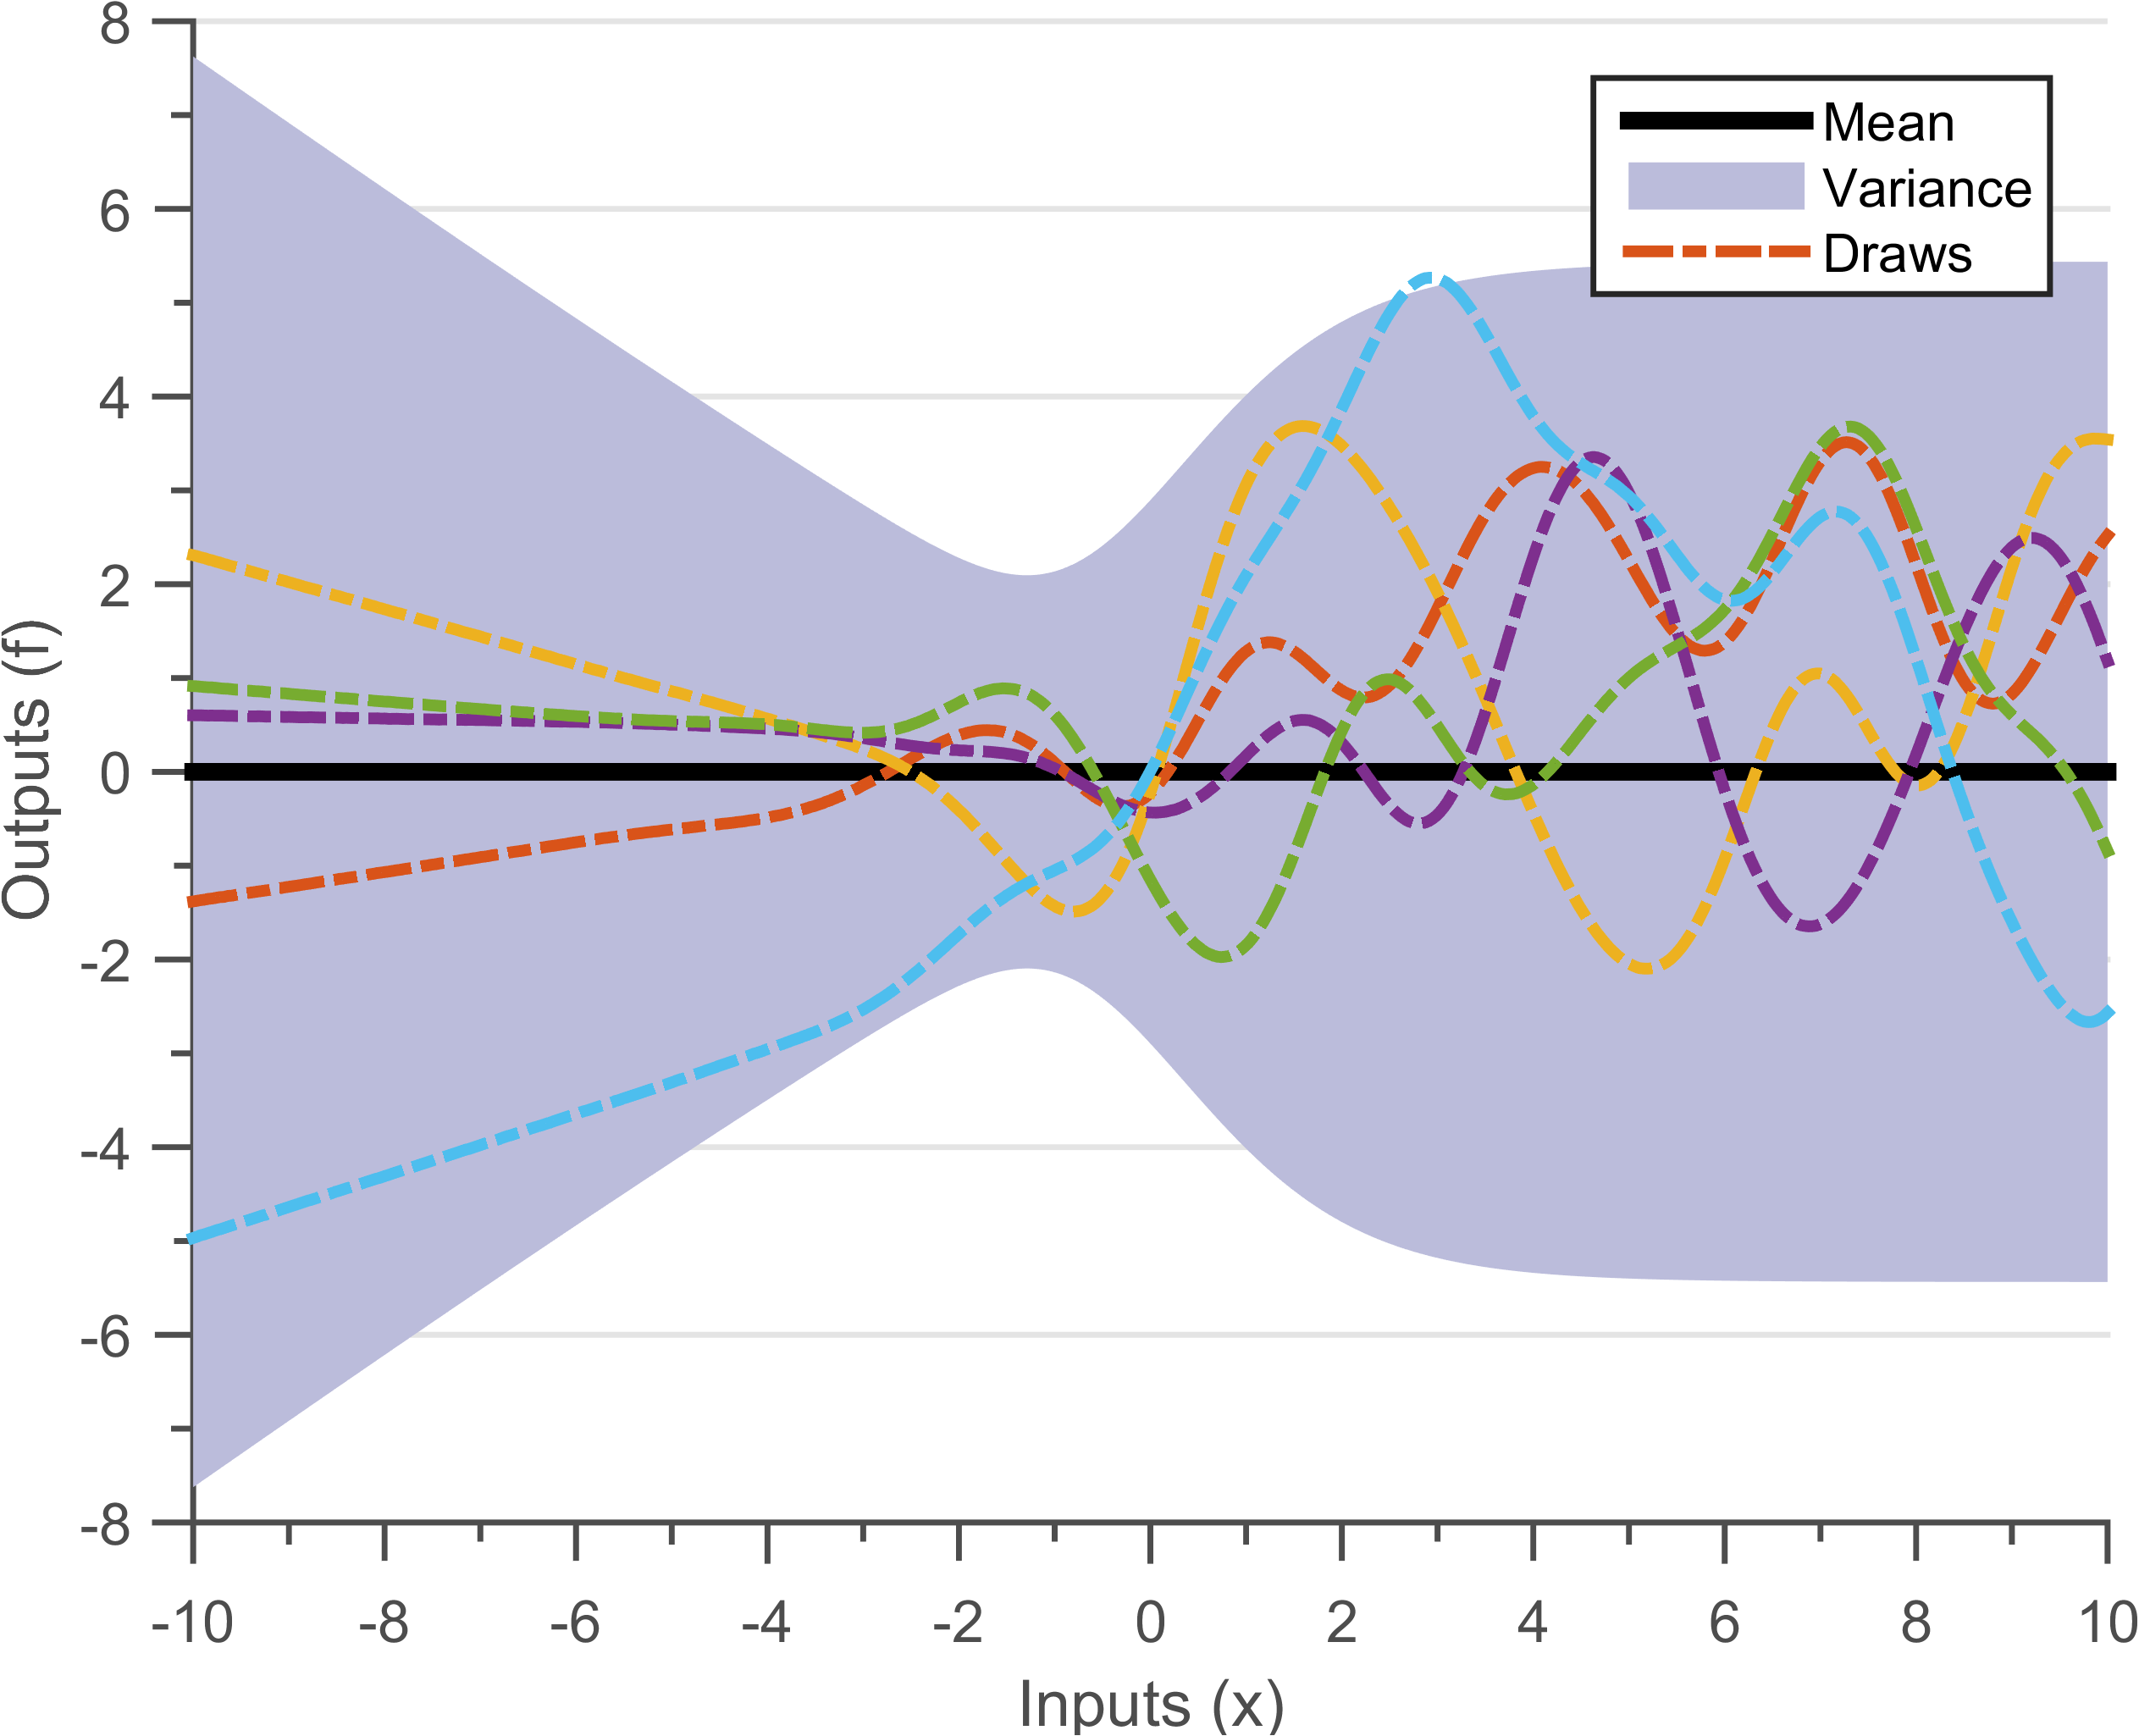
\includegraphics[width=0.29\textwidth]{imagesPart2/drawsCP1}\label{subfig:drawsCP1}}\quad
    \subfigure[]
  {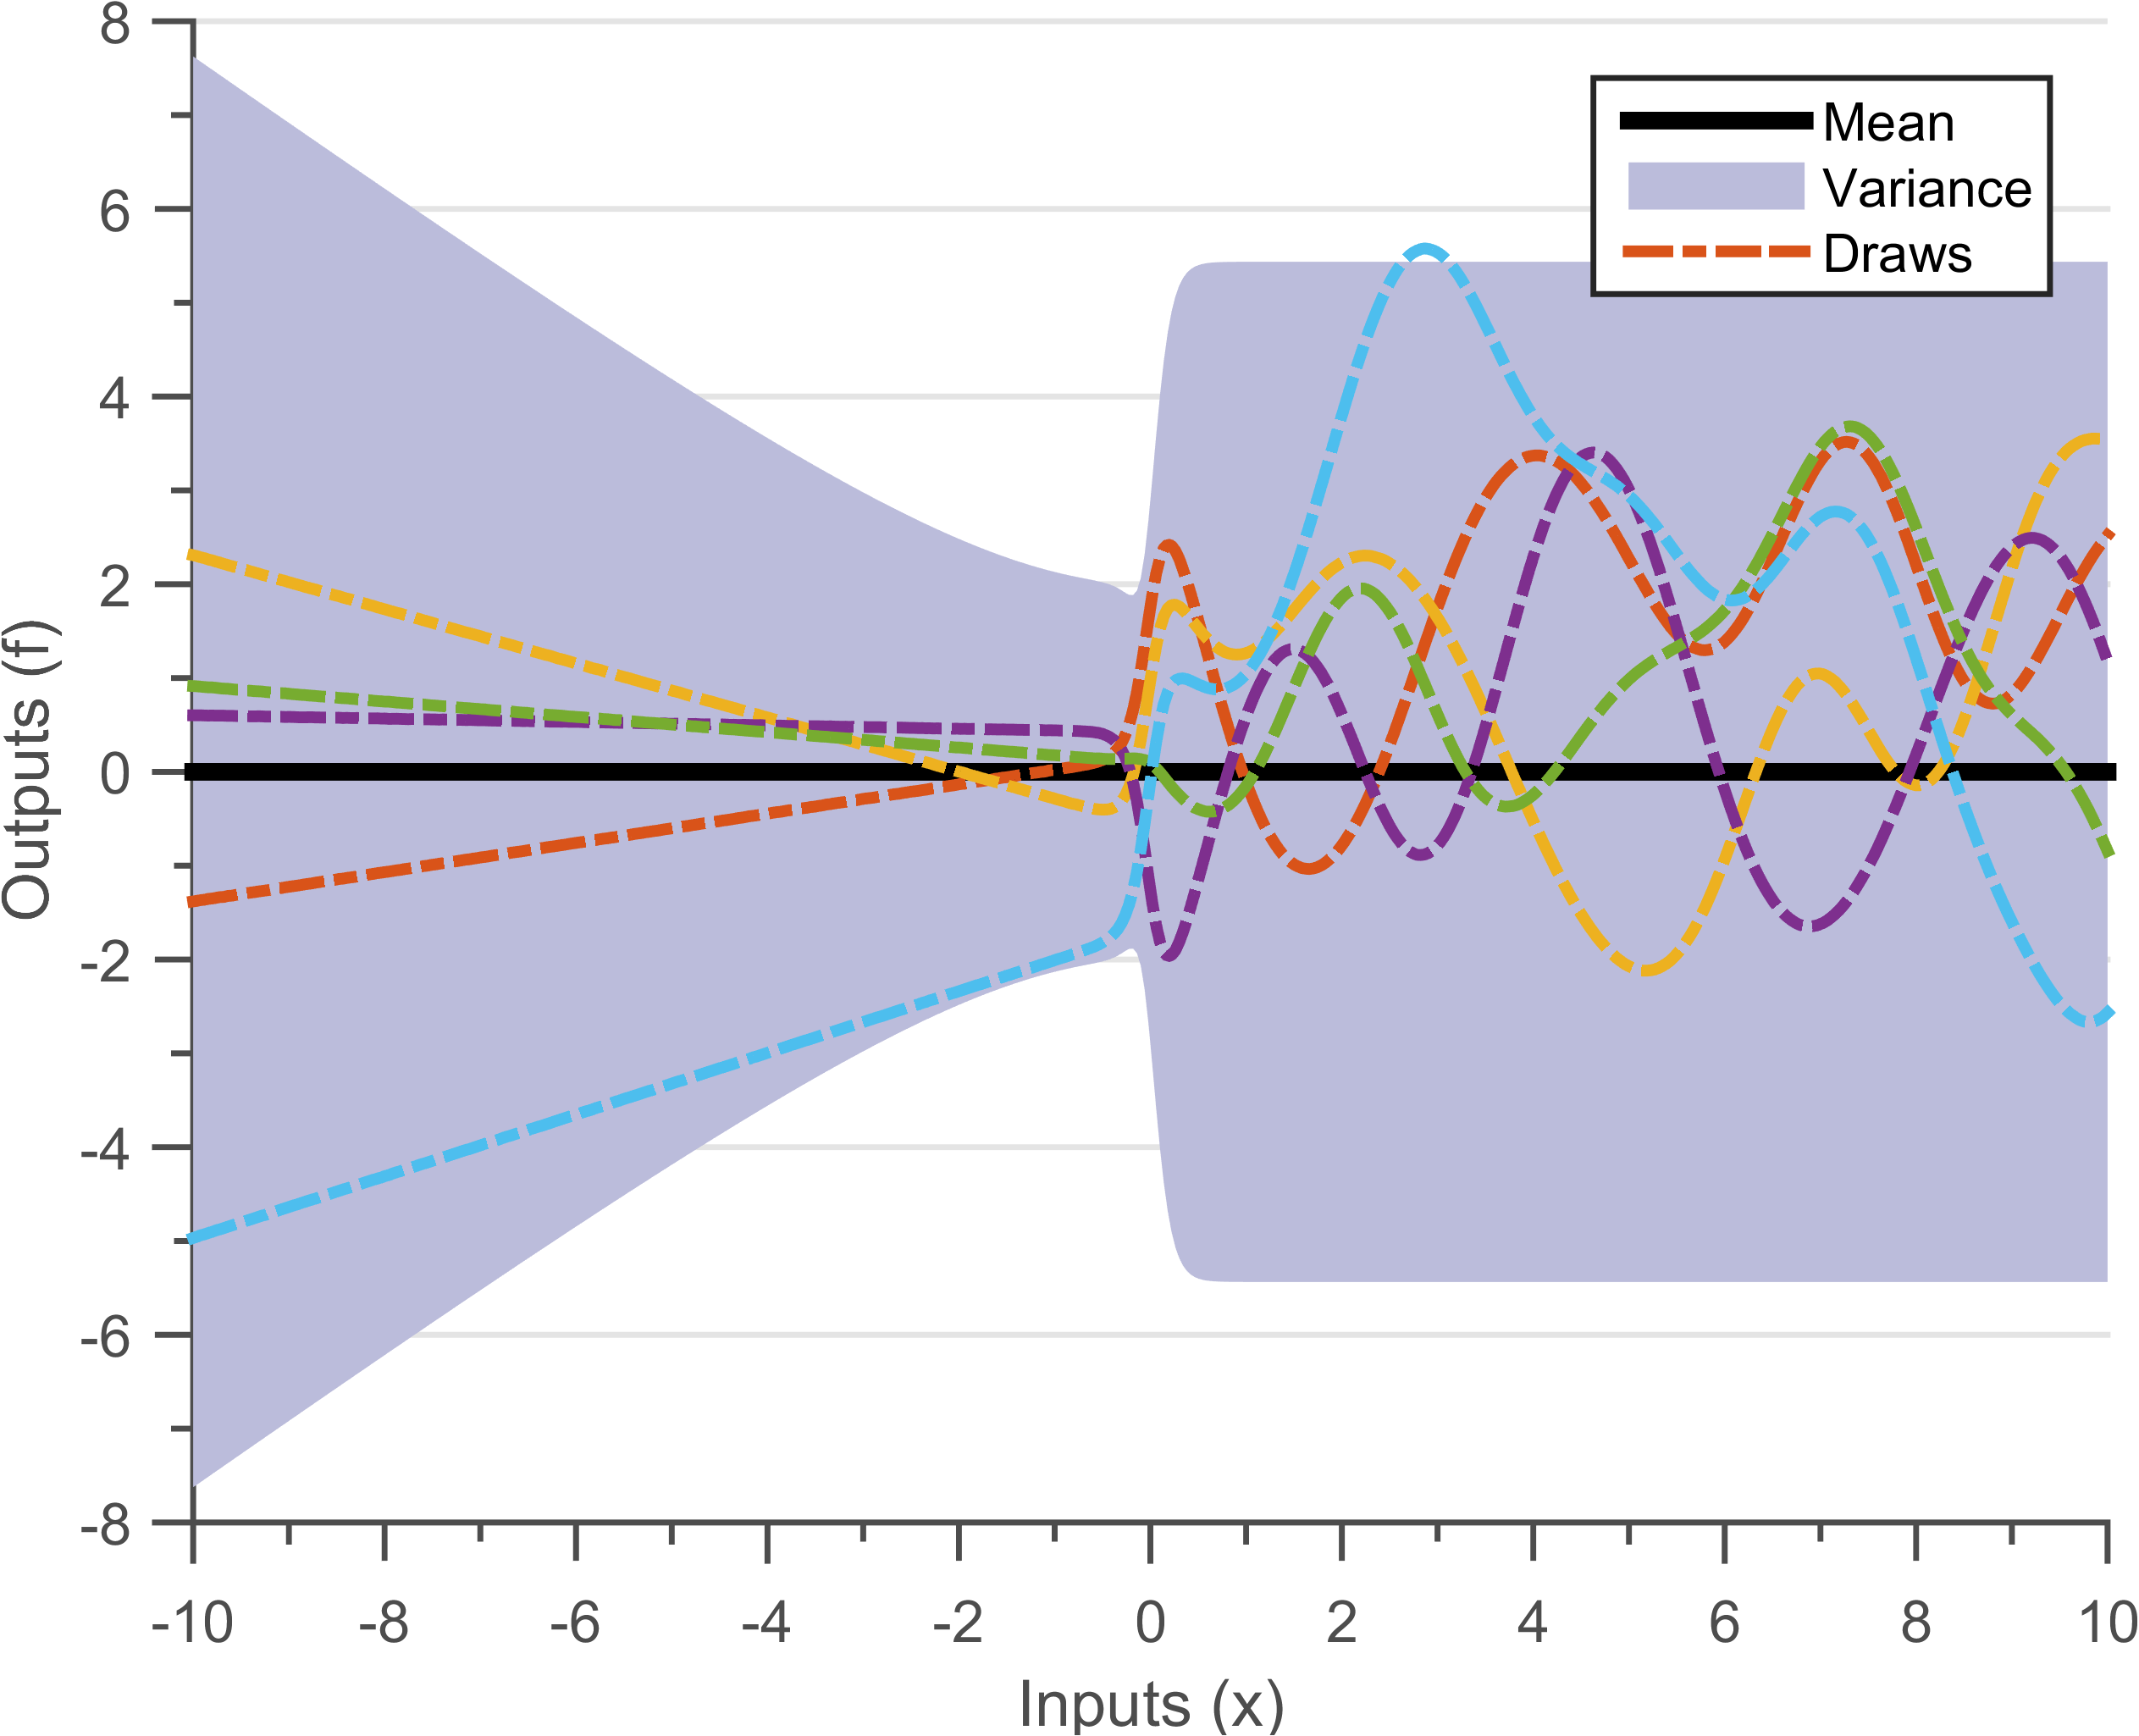
\includegraphics[width=0.29\textwidth]{imagesPart2/drawsCP10}\label{subfig:drawsCP10}}\quad
  \subfigure[]
  {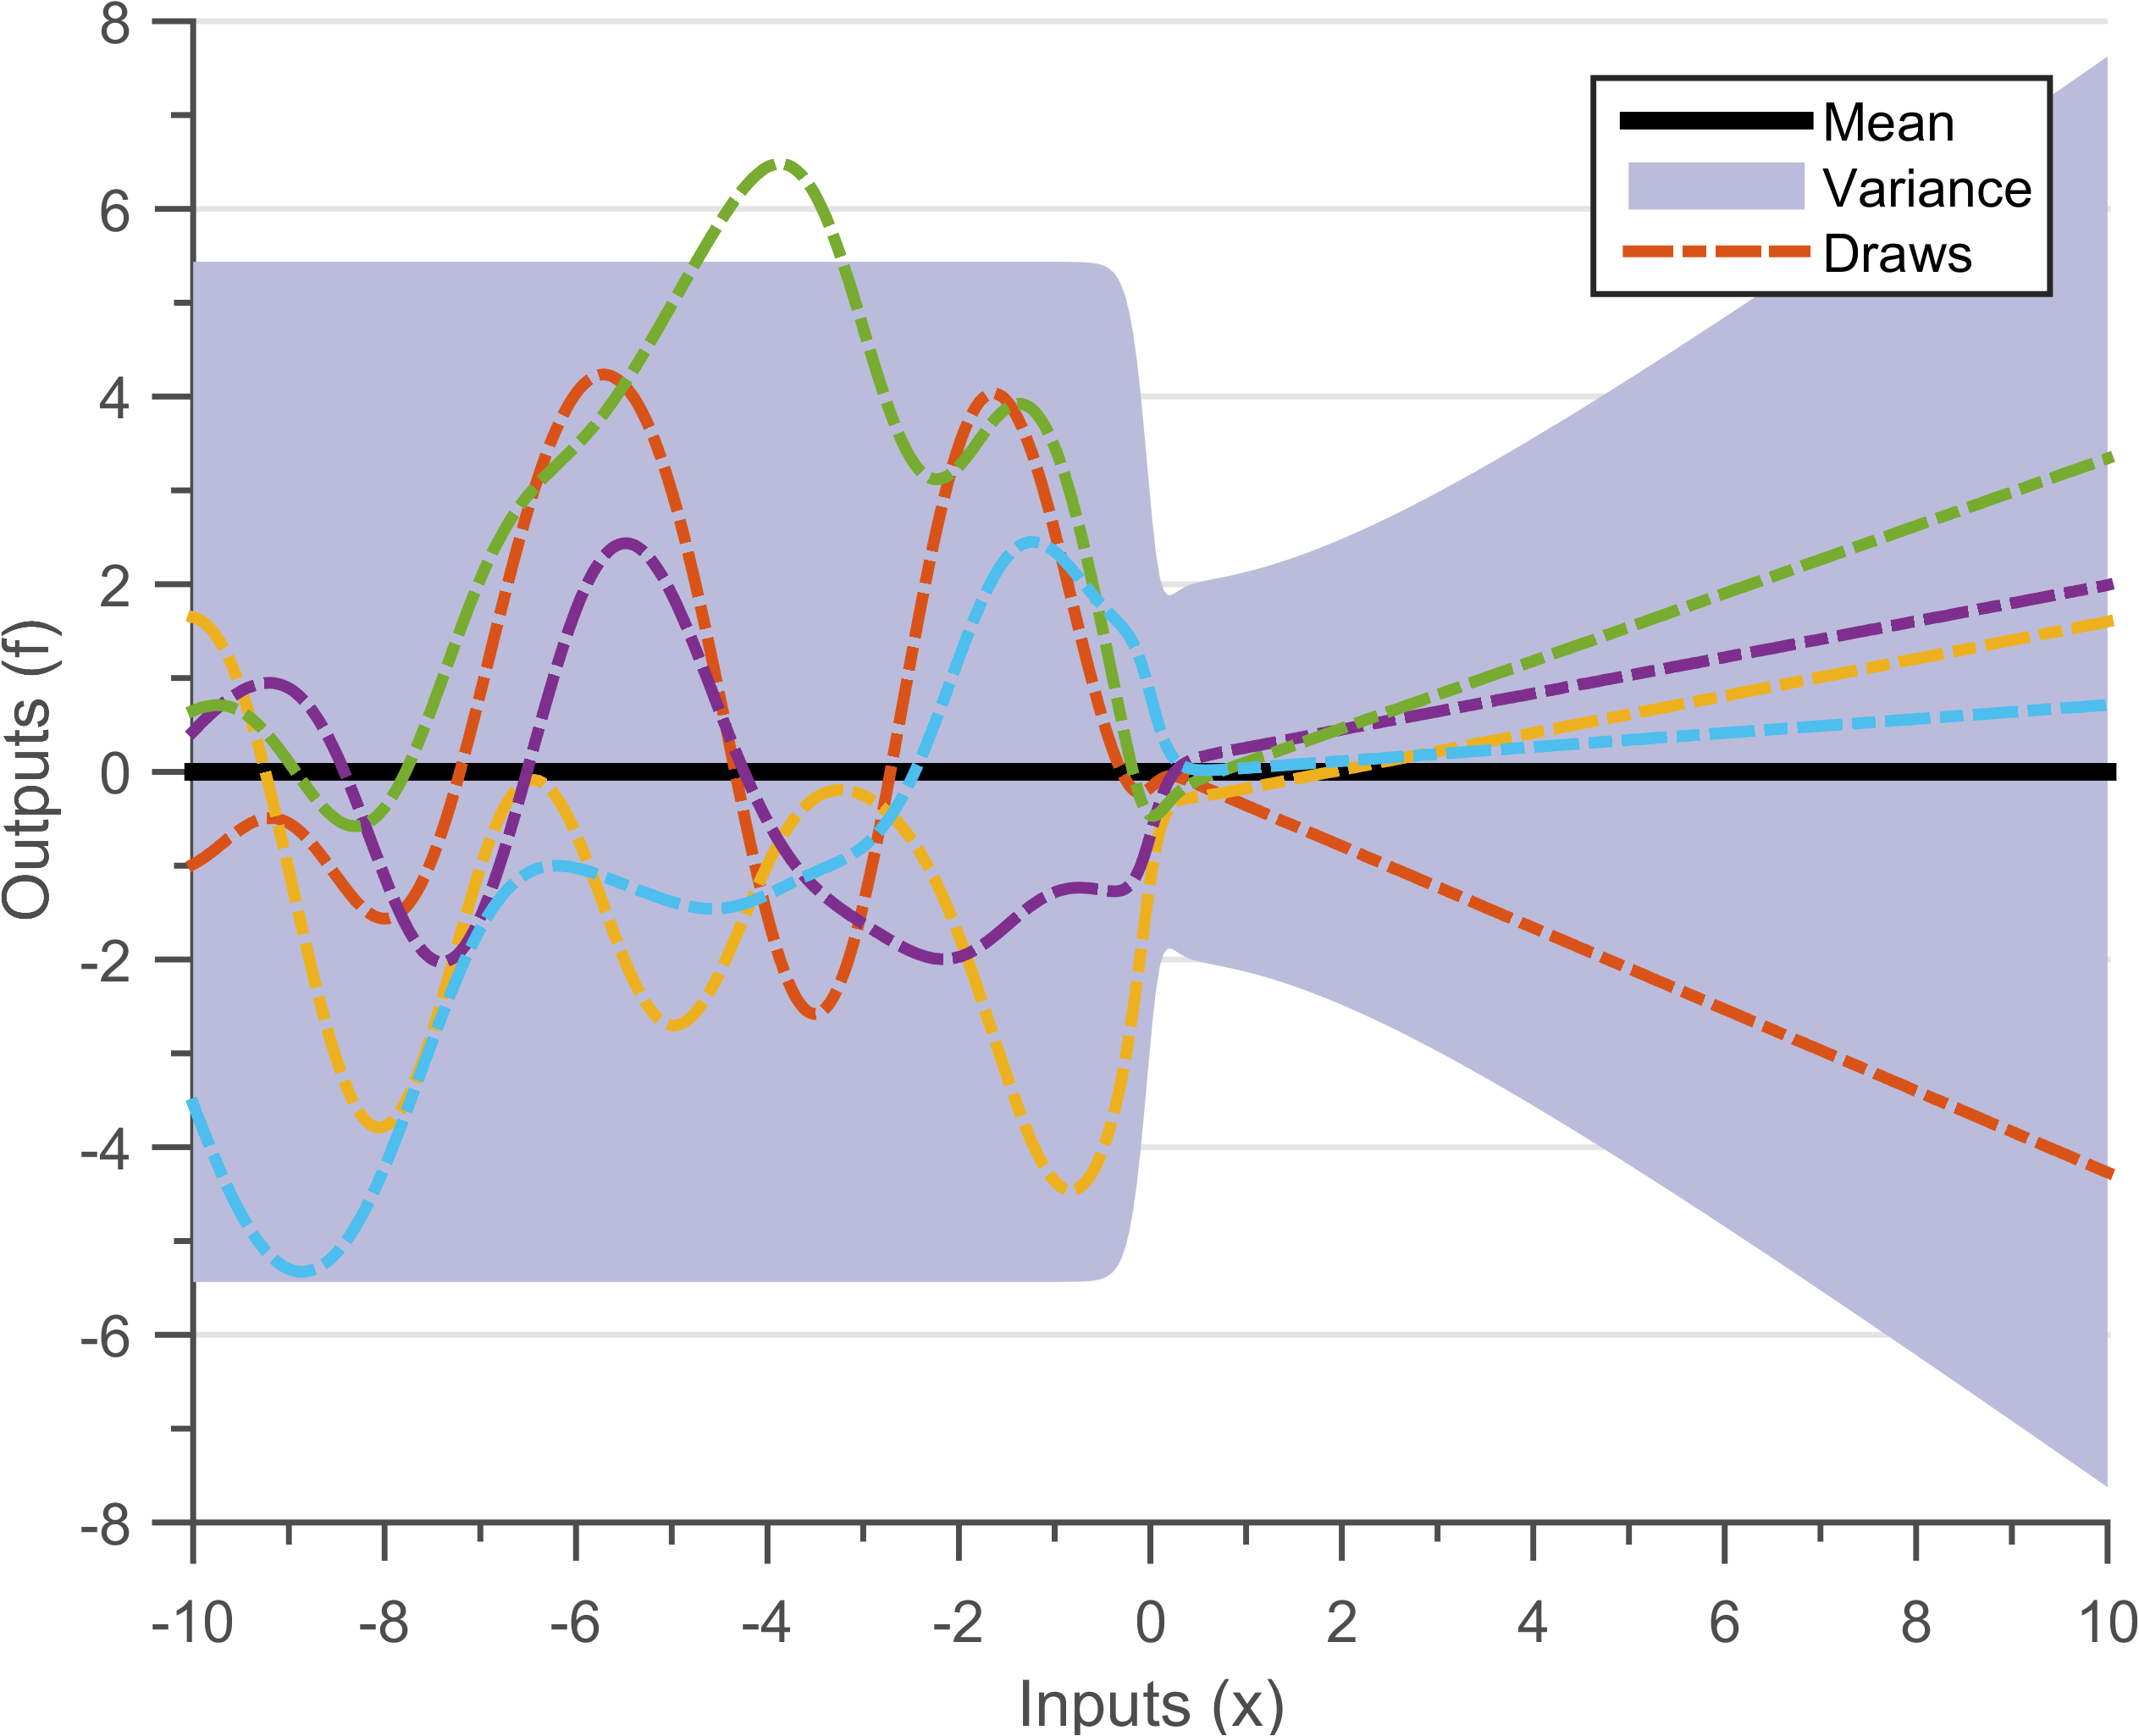
\includegraphics[width=0.29\textwidth]{imagesPart2/drawsCPMinus10}\label{subfig:drawsCPMinus10}}\quad
  \caption{}
\end{figure*}

\subsection{Application: Identifying onset of non-linearity  using CP kernel}\label{subsubsecCh4ApplicationCP}
In several physical processes, there is an equilibrium condition. Near this equilibrium, a linear approximation is performed and when the assumptions start failing a non-linear domain is observed. This basic approximation is made in experiments such as: lift vs alpha curves; estimation of Young's Modulus; basics of control theory. The value of these physical parameters slope (eg. Young's Modulus) and position of changepoint (eg. plasticity) are progressively fed into further simulations. 

These basic physical properties define the general characteristics of the field. The parameters are then later fed into more complex designs and used as an input into particular mesh elements (remember induction vs deduction \ref{sec:machineLearning}). The values of slopes and position of change-point are approximated by engineering judgement. 

\begin{figure}[!ht]
  \centering
    \subfigure[]
	    {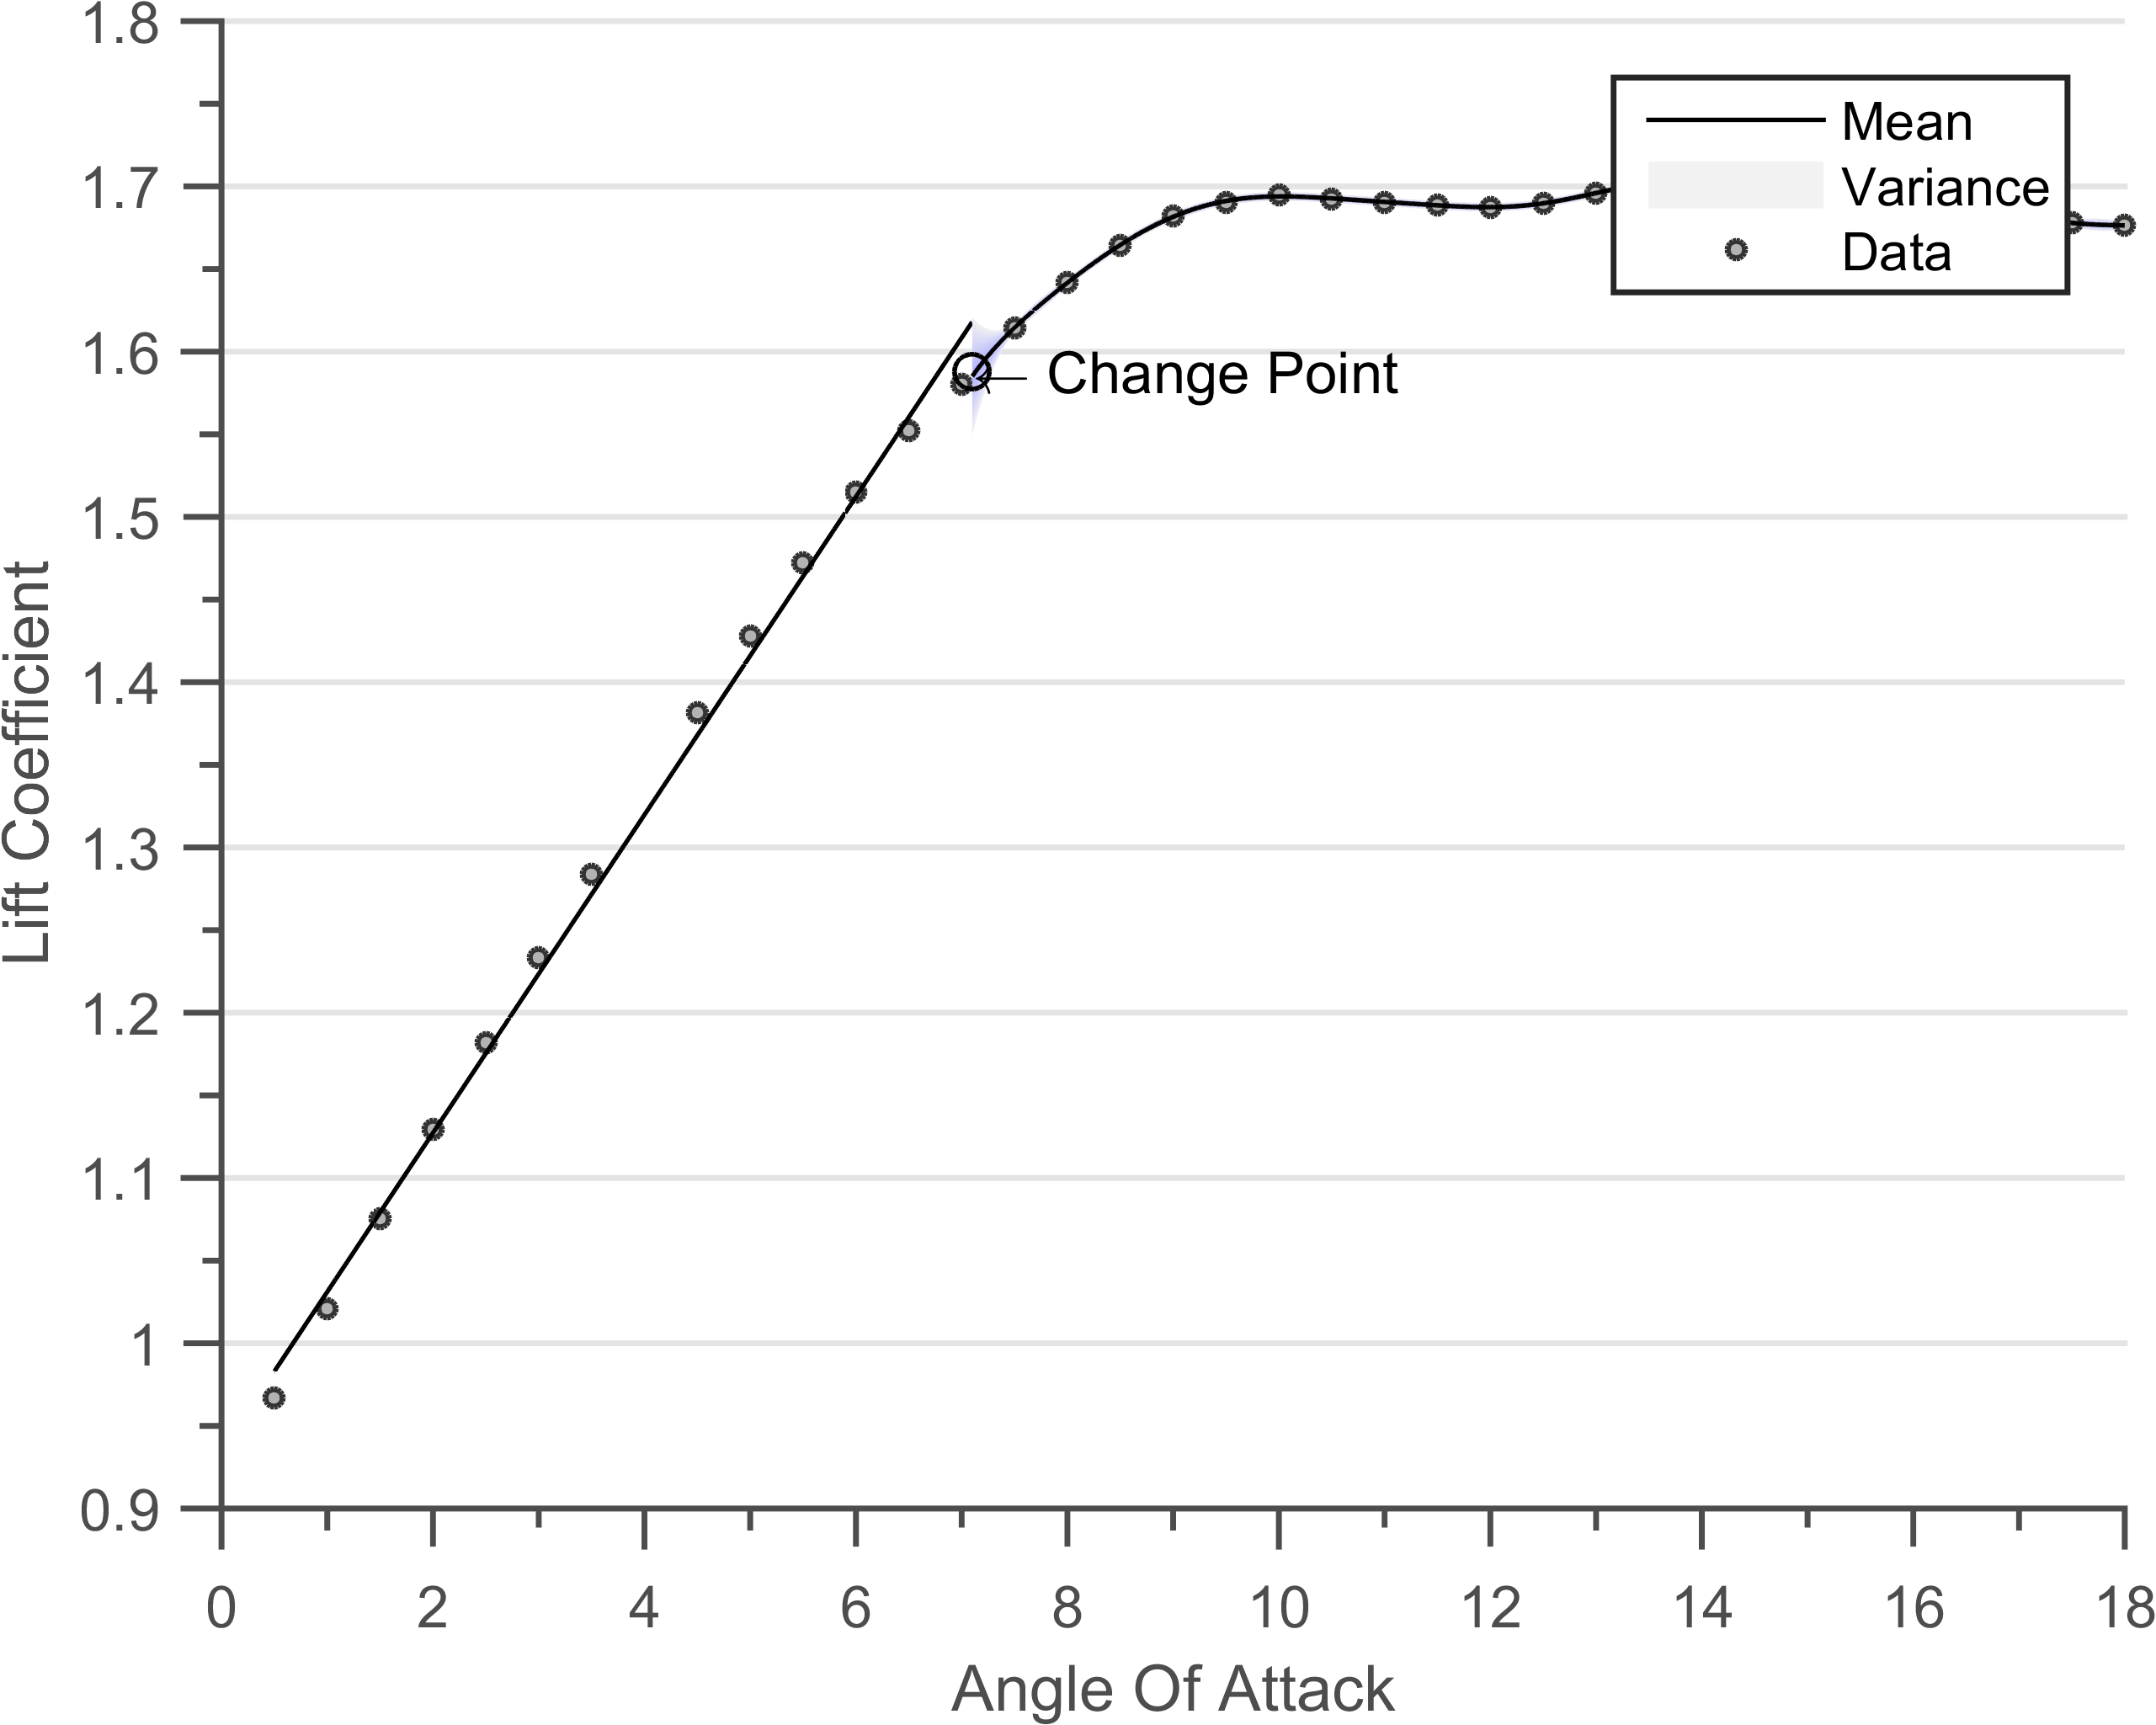
\includegraphics[width=0.45\textwidth]{imagesPart2/clAlphaCovCP}\label{subfig:clAlphaCovCP}}\quad
    \subfigure[]
	    {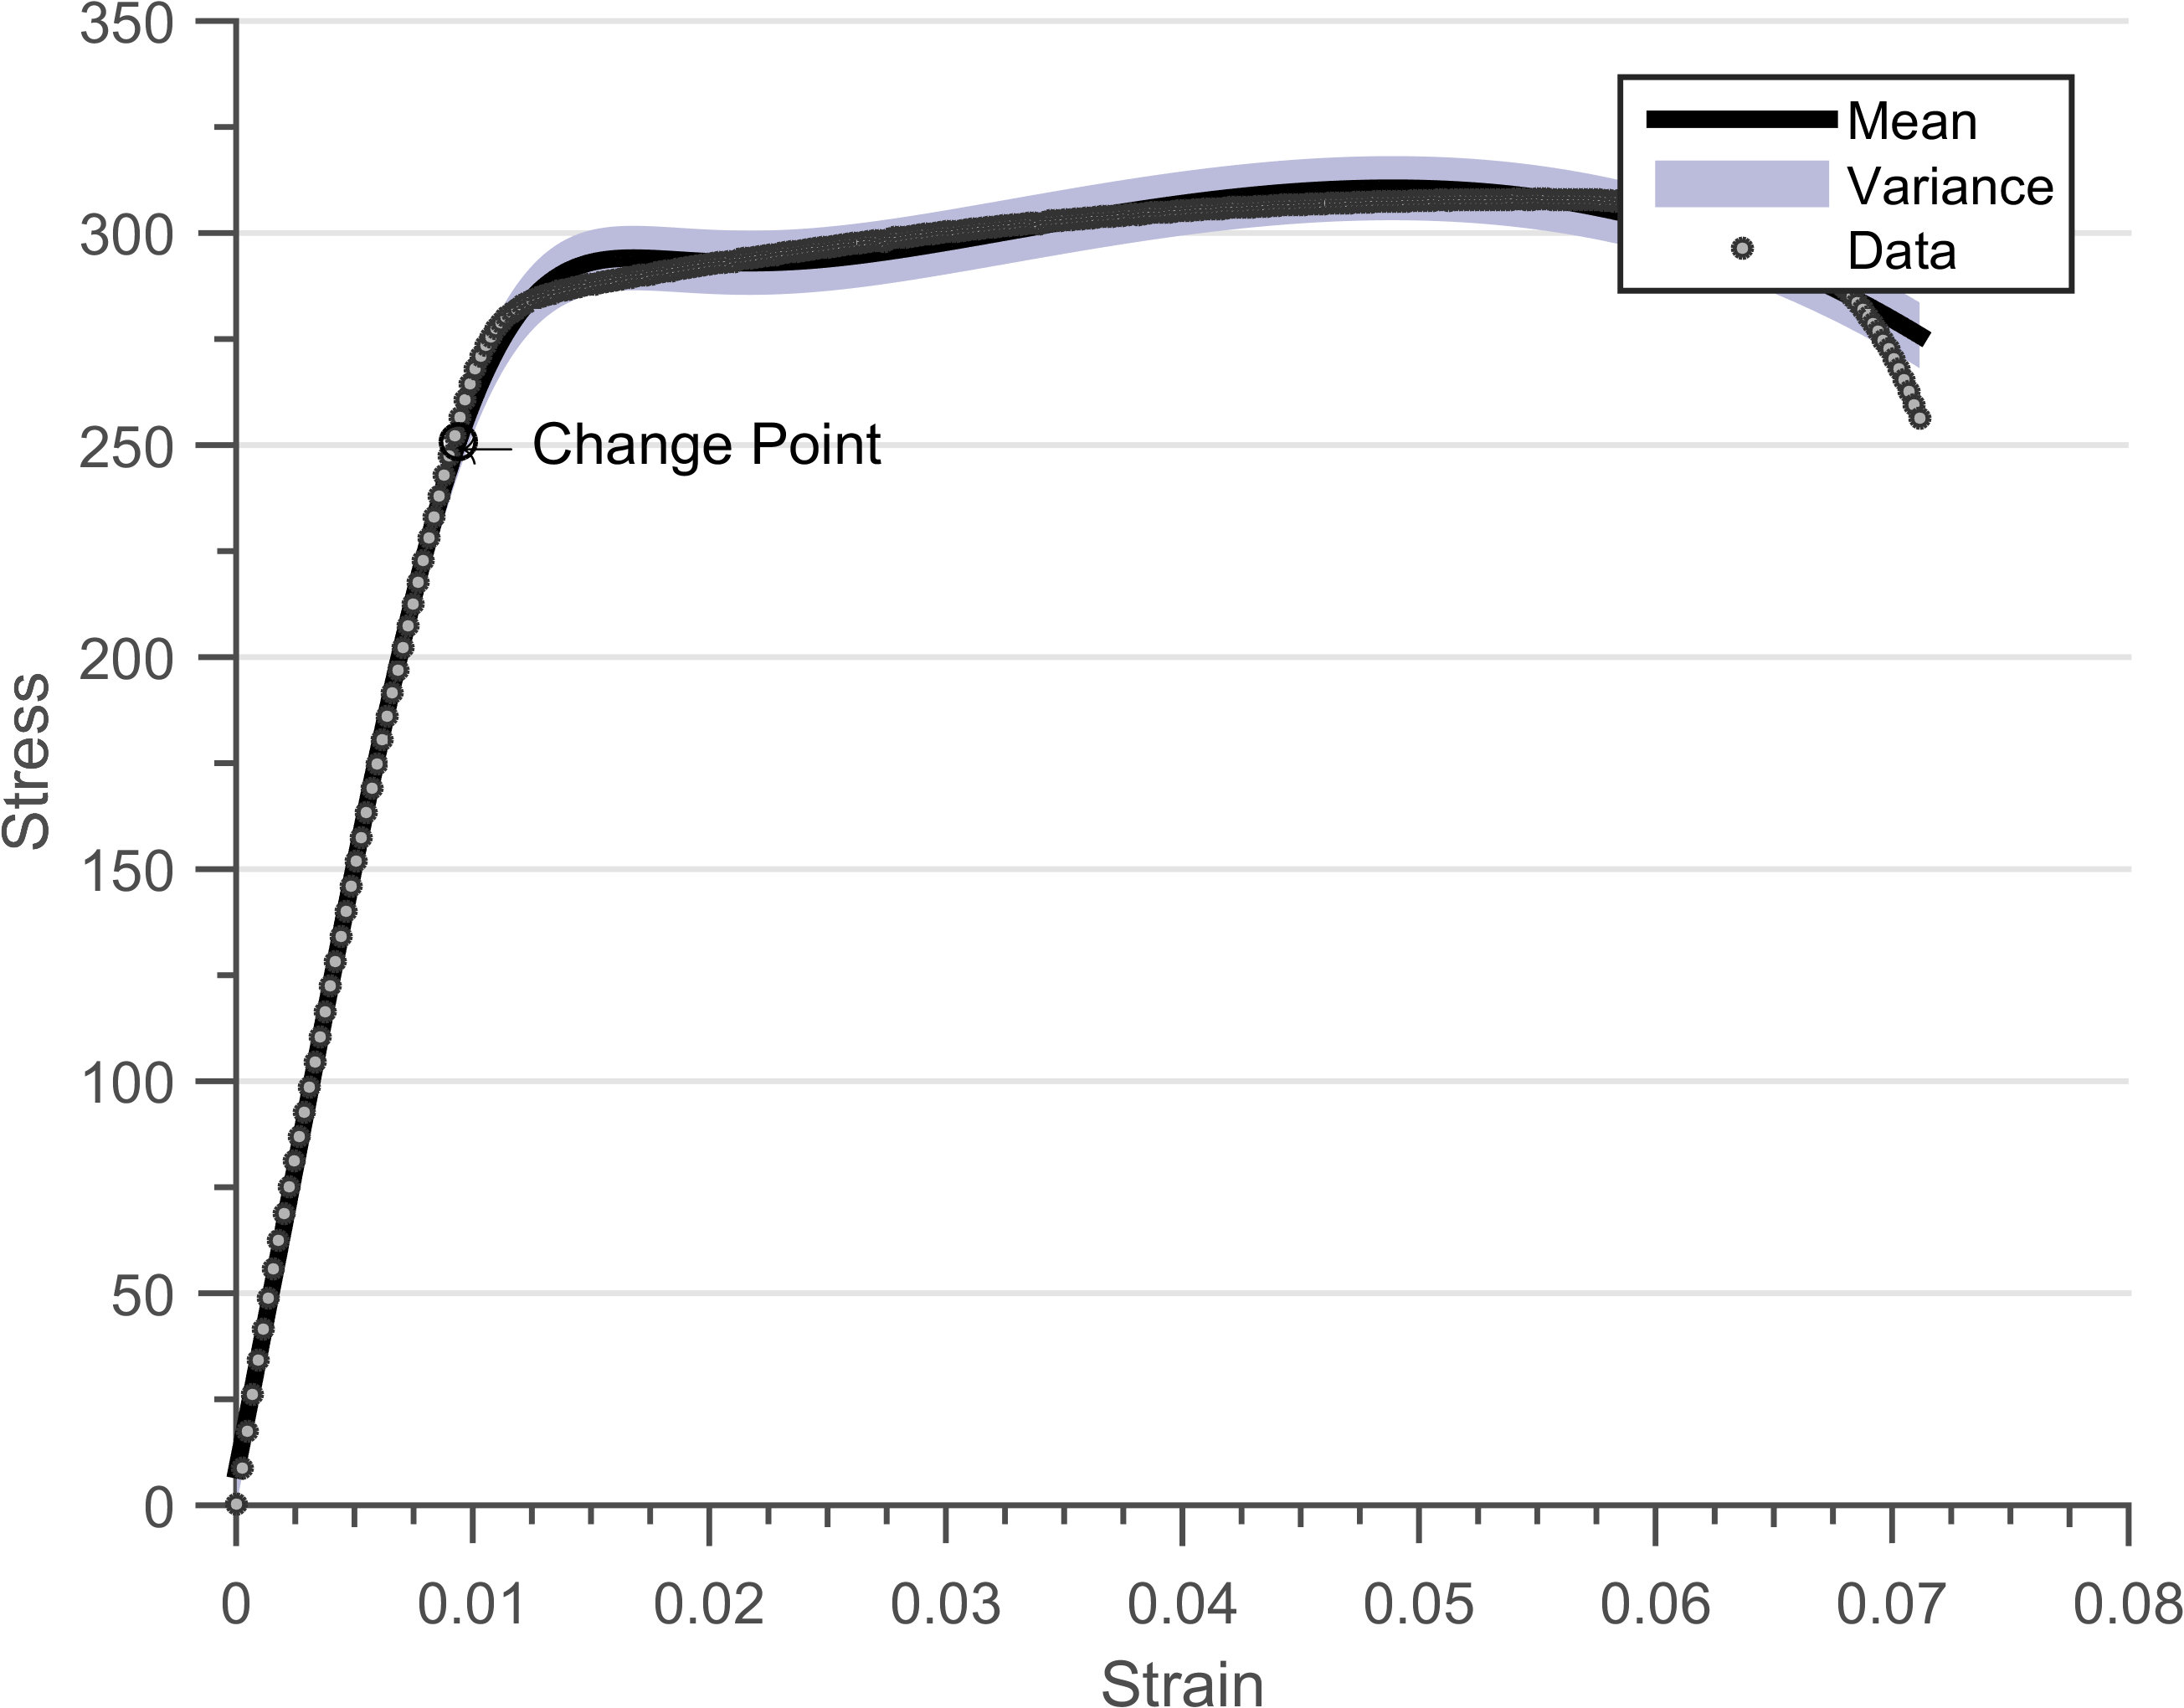
\includegraphics[width=0.45\textwidth]{imagesPart2/stressStraincovCPPlot}
	    \label{subfig:stressStraincovCPPlot}}
	    \caption{}
\end{figure}


We tried to solve the problem of estimating the lift coefficient using Gaussian Process. Using the changepoint kernel which transitions from linear domain (linear kernel) to non-linear domain (SE kernel), prior assumptions of the problem were encoded in the kernel structure. Open source data for the lift vs alpha curves for the NACA 0012 airfoil were chosen. Fig: \ref{subfig:clAlphaCovSE} shows the regression of the data using SE kernel. Fig: \ref{subfig:clAlphaCovCP} regression of the same dataset using the CP(linear, SE) kernel. 

We can observe that the algorithm predicts a changepoint for the dataset. This is the point with where the linear assumptions start failing, according to prior information. The marginal likelihood of CP(linear, SE) kernel is rigged with many local minimas. The algorithm tries to put a changepoint at every observation point. Hence using a global optimizer is advised. The changepoint kernel is also very numerically unstable hence cross-validating the learners is also very important (model ensembles \ref{subsec:modelEnsembles}). The results of this study will be presented in the SIAM Uncertainty Quantification 2016 Conference.


\section{Discussion}

\textbf{A table to list common  }
%%% Local Variables: 
%%% mode: latex
%%% TeX-master: "isae-report-template"
%%% End: 

